\section{Frequency control} \label{sec:frequency_control}

In modern systems, control over the processor frequency can be done by hardware with independent circuits as well as by software. For that, there is the Advanced Configuration and Power Interface (ACPI) an open standard adopted by operating systems to configure hardware components related to power management.

In the ACPI two important states for the DVFS are defined that optimize the energy consumption. They are "C", which is activated when the processor is not executing any instructions, and "P", which is activated while the processor is operating. These states have several levels and at each level the frequency and voltage are changed.

State P starts at level P0, where frequency and voltage are the maximum possible, then P1, where both decrease, until reaching the last state, Pn, where frequency and voltage are the lowest possible. The change of state depends on the level of utilization of the processor. To stay in each state, the level of processor usage must be within specific limits. After exceeding these limits for a certain time, the state will change to the next state corresponding to that new level of processor usage. The number of possible states depends on each manufacturer.

After an idle time, the processor begins to activate C states, starting with C0 where it is still fully active, then moving to C1, where some features are disabled, up to Cn, where all possible features are disabled. The ACPI standard establishes the functionalities that can be disabled between level C1 and level C3, as seen in Table \ref {tab:states_c}. The other levels are specific to each manufacturer.

\begin{table}[H]
\centering
\begin{tabular}{| l | l | l |}
\hline
Mode & Name & Functionality \\ \hline
C0 & operating state & Active processor \\ \hline
C1 & Halt & Stop executing instructions \\ \hline
C2 & Stop-Clock & Disable the internal clock \\ \hline
C3 & Sleep & Disable cache coherence \\ \hline
\end{tabular}
\caption{C states}
\label{tab:states_c}
\end{table}

In state C, the higher the level the greater the energy savings, but returning to the fully functional level is more difficult. In states P, there is a trade-off between performance and energy savings. \cref{fig:p_state} best illustrates the change of states, in which we can see which parts of the circuits are deactivated in states C, the latency to return to the active state, power consumption and also shows the relationship of states P with often.

\begin {figure} [H]
\centering
\begin{subfigure}[t]{0.5\textwidth}
\centering
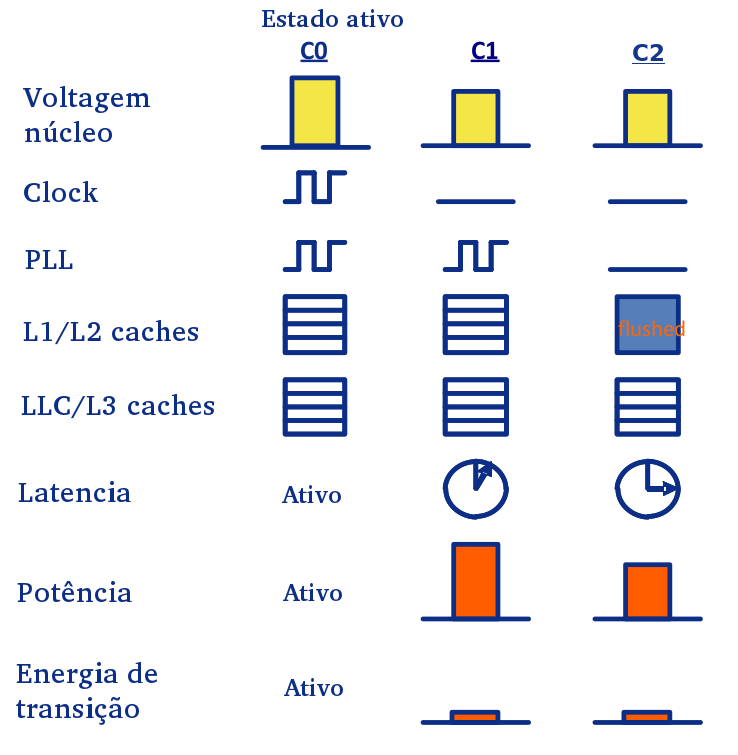
\includegraphics[width=\columnwidth]{intro/figures/c_states}
\caption{C states}
\end{subfigure}%
~
\begin{subfigure}[t]{0.5\textwidth}
\centering
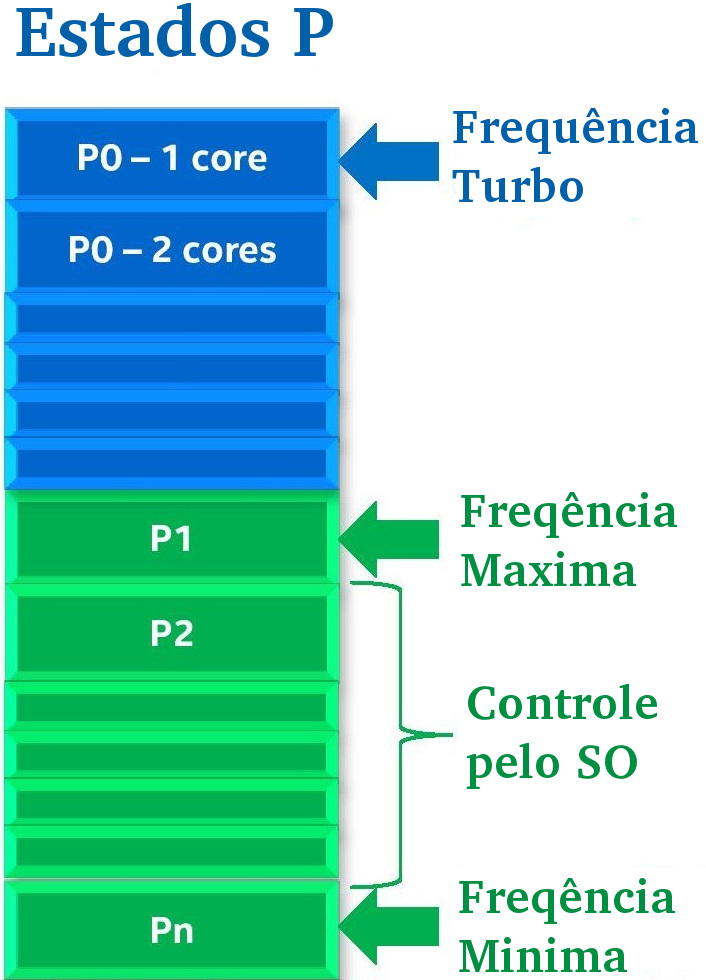
\includegraphics[width=\columnwidth]{intro/figures/p_states}
\caption{States P}
\end{subfigure}
\caption {Illustration of states C and P} {Altered image from \protect \url {https://www.thomas-krenn.com/en/wiki/Processor_P-states_and_C-states}}
\label{fig:p_state}
\end{figure}


% Are states C and P orthogonal, do they operate independently?

For this management, the operating system provides in the user space a way to control the frequency. This work used an operating system that has Linux as its core.

Linux is compatible with several modern architectures and is widely used in servers, smartphones and supercomputers. It was based on the UNIX system which has the philosophy of treating everything on the system as a file, including settings and input and output devices, such as keyboard, mouse and hard drive. Another important feature is that it is modular and parts of the system can be loaded or removed during execution.

On Linux there are several frequency management options \cite {Brown2005ACPILinux}. The main ones are acpi-cpufreq, Intel P-state, AMD powernow. In this work, acpi-cpufreq is used, which is standard and allows direct control of frequency through system files. Acpi-cpufreq is a Linux module that uses implemented policies that dynamically decide the frequency to be used. Some of these policies are:

\begin{itemize}
\item Performance - configured as often as possible
\item Powersave - configured as low as possible
\item Userspace - the user chooses the frequency to be used
\item Ondemand - controls the frequency depending on the processor load. When the load increases the frequency also increases accordingly.
\item Conservative - similar to Ondemand but more smoothly, the frequency increase is continuous instead of jumping.
\end{itemize}

\section{Power consumption monitoring} \label{sec:power_consumption_monitoring}
The Running Average Power Limit (RAPL) and Intelligent Platform Management Interface (IPMI) interfaces were used to measure the power consumed. described in \cite{IPMI2013ConfigurationGuide}.

\subsection{IPMI}
IPMI \cite{IPMI2013ConfigurationGuide} is a set of specifications for autonomous subsystems that provides processor, firmware and operating system independent management and monitoring. The use of IPMI allows system administrators to avoid having to travel to the server location, which is often far away, to perform their tasks. Also, servers are located in places with low temperature and with a lot of noise due to the ventilation system, and one should avoid spending too much time in these places. With remote management, it is possible to turn the system on and off, remotely access the (BIOS) and reinstall the system in case of any serious failure.

\begin{figure}[H]
\centering
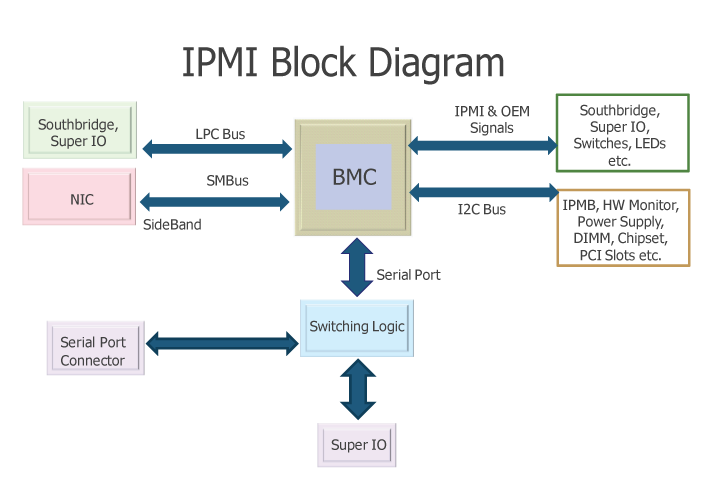
\includegraphics[height = 7.5cm] {intro/figures/IPMI-Block-Diagram.png}
\caption{IMPI diagram} {Image taken from \protect \url {https://pt.wikipedia.org/wiki/Intelligent_Platform_Management_Interface}, the main components of IPMI and how they communicate are shown}
\label{fig:IPMI}
\end{figure}

Access to the IPMI network can be done using the HTTP protocol or a tool made available by the manufacturer (ipmitool), which also performs access via the network. It is also used to monitor the status of the platform with a set of sensors coupled with system temperatures, voltages, fans and power supplies.

\subsection{RAPL}

Modern Intel microprocessors, based on the SandyBridge architecture, include the RAPL \cite {Rotem2012Power-managementBridge, Hahnel2012RAPL, Hackenberg2015AnProcessor} interface designed to limit the use of energy on a chip while ensuring maximum performance. This interface supports energy measurement capabilities through an integrated circuit that estimates energy use based on a model driven by architectural event counters for all components. It also provides temperature readings and current leak models. Estimates are made available in model-specific registers (MSR), updated in milliseconds. The energy estimates offered by RAPL were validated by Intel, which showed excellent results.

\section{Case-Study Architecture} \label{sec:casestudyarchitecture}
The experiments were executed in one computer node equipped with two Intel Xeon E5-2698 v3 processors with sixteen cores each and two hardware threads for each core. 
The overall view of the architecture is shown in \cref{fig:architecture}.
The maximum non-turbo frequency was 2.3 GHz, and the total physical memory of the node was 128 GB (8 $\times$ 16 GB). Turbo frequency and hardware multi-threading were disabled during all experiments. The operating system used was Linux CentOS 6.5, kernel 4.16. 

\begin{figure}[H]
	\centering
	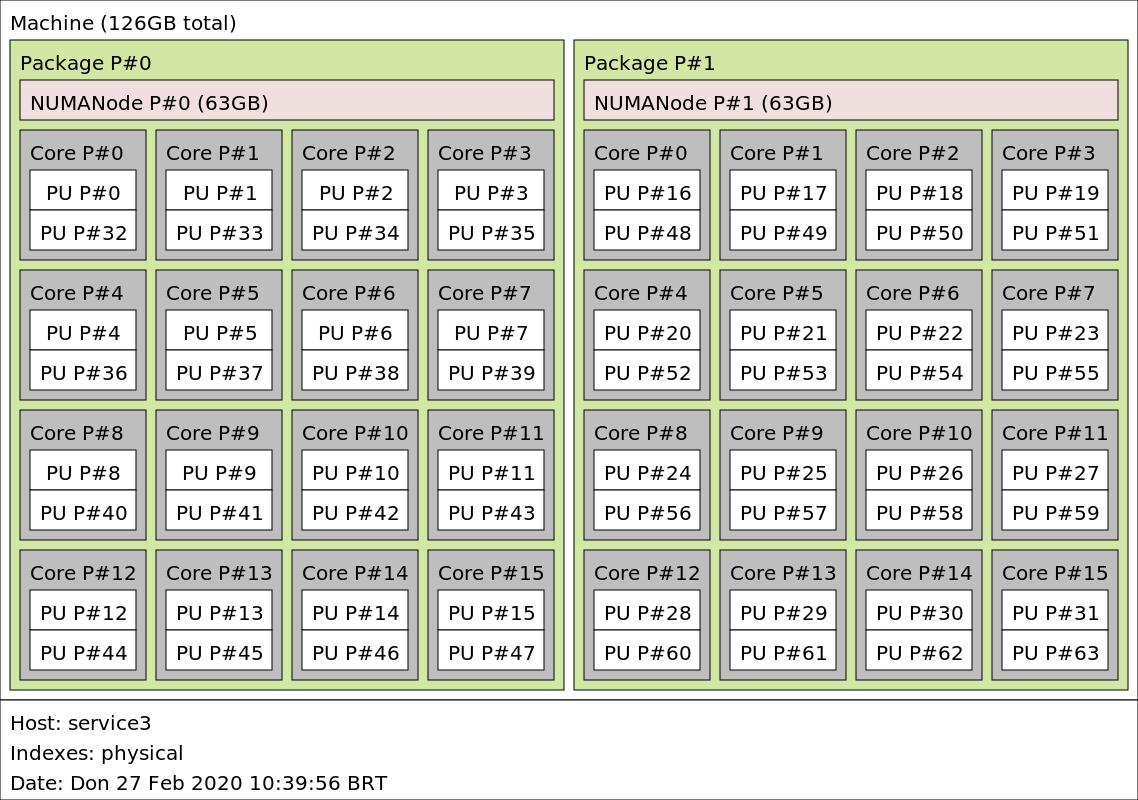
\includegraphics[width=\columnwidth]{models/figures/architecture.png}
	\caption{Node architecture (the image was made with the lstop application).}
	\label{fig:architecture}
\end{figure}

The Linux kernel has many different policies for power management, depending on the driver. In the default driver, the acpi-cpufreq, the options are Powersave, Performance, Ondemand, Conservative, and Userspace. Each governor has a policy on how the frequency is selected. In this investigation, the frequency control was performed using the Userspace governor, which allows the user or any userspace program to set the CPU to a specific frequency. The core control was accomplished by modifying the appropriate system files with the default CPU-hotplug driver.

The architecture was equipped with the intelligent platform management interface (IPMI), a set of interfaces allowing out-of-band management of computer systems and platform-status monitoring via the local network~\cite{Schwenkler2006IntelligentInterface}. It can monitor variables and resources, such as the system's temperature, voltage, fans, and power supplies, with independent sensors attached to the hardware.

\section{Case-Study Applications} \label{sec:casestudyapplication}
The applications blackscholes, bodytrack, canneal, dedup, fluidanimate, freqmine, raytrace, swaptions, vips and x264 from the PARSEC \url{https://parsec.cs.princeton.edu/download.htm} (accessed on 20 February  2020) parallel benchmark suite, version 3.0~\cite{Bienia2008TheSuite}, OpenMC \cite{Romano2015OpenMC:Development} and LINPACK (HPL) \cite{Dongarra1988TheExplanation}, were chosen as case studies. The PARSEC benchmark focused on emerging workloads and was designed to represent the next-generation shared-memory programs for chip-multiprocessors. It covers an ample range of areas, such as financial analysis, computer vision, engineering, enterprise storage, animation, similarity search, data mining, machine learning, and media processing. The OpenMC and the LINPACK are two classic HPC programs.

%The other two experiments use applications Raytrace~\cite{Bienia2008} and OpenMC~\cite{Romano2015OpenMC:Development}. Raytrace is an application addressed on rendering photorealistic scenes. It is available on the PARSEC Benchmark suite, version 2.0. The PARSEC benchmark, focused on emerging workloads, represents the next-generation shared-memory programs for chip multiprocessors. It covers a wide range of areas such as financial analysis, computer vision, engineering, enterprise storage, animation, similarity search, data mining, machine learning, and media~processing.
%
%\textls[-20]{{OpenMC is an application that implements the Monte-Carlo method to simulate the transport of neutrons and photons. It is a classic program aimed at high-performance computing.}}

\section{Validation the framework}\label{sec:validation_the_framework}
In this Section, we discuss the measurements and simulation results for three distinct cases, including two real applications. We also demonstrate how external libraries and standalone visualization tools can be used to render the collected data and investigate performance aspects such as the program's scalability capacity.

\subsection{Configuration} \label{subsec:configuration_pascal}

We used three experiments to assess the tool and demonstrate its ability to support analysis aimed at observing parallel scalability. The first includes a runtime imbalance between processing units in a specific parallel region. In this case, the objective is to present how the analyzer helps users observe the impact of the inefficiency of a code part on the whole program. The code for this experiment is presented in \cref{lst:codes_regionscomparison}. It consists of two simple parallel regions with the same functionality that divide the iterations of a loop between the available threads. The difference between the regions lies in the strategies used to manipulate the sum variable, used in the example to store the values of the calculations performed in each thread. We assume that the {\tt anyop()} function, in this case, invariably has the same runtime in all function calls.

The command presented on \cref{lst:pascal_usage_ex} was used as base to perform experiments. For the experiment of \cref{lst:codes_regionscomparison}, we use just the parameters {\tt -c}, {\tt -r}, {\tt -t}, {\tt -a} and {\tt -o}, including the 64 value to {\tt -c} option.

\lstset{style=ccodestyle, frame=tb}
\begin{lstlisting}[label={lst:pascal_usage_ex}, language=bash, caption={Command line showing how experiments were run through a terminal.}]
	analyzer 
	application
	-c 1,2,4,8,...,32 # threads/cores
	-r 3 # number of repetitions
	-t auto # automated instrumentation
	-a 1 # aggregation mode
	--ipmi ip user psswd # energy sensor
	--idtm 5 # idle time between runs
	--dhpt # disable hyper-thread
	--dcrs # disable cores
	--ipts ... # application specific inputs
	-o application.json # output file
\end{lstlisting}

\lstset{style=ccodestyle, frame=tb}
\begin{lstlisting}[label={lst:codes_regionscomparison}, language=C, caption={Sample code used to visualize the impact of regions on program scalability.}]
	int main(int argc, char **argv) {
		unsigned long sum = 0;
		int ops = atoi(argv[1]);
		
		#pragma omp parallel for schedule(static) reduction(+: sum)
		for (int i = 0; i < ops; i++)
		sum += anyop();
		
		#pragma omp parallel for schedule(static)
		for (int i = 0; i < ops; i++) {
			#pragma omp critical
			sum += anyop();
		}
	}
\end{lstlisting}

The command return a .json file with all the information necessary for our analysis. We can quickly generate tables with the collected data from this file, thus supporting observation and analysis of scalability, energy trends, and model fitting. The code described in \cref{lst:regtab} and \cref{tab:regtable_dedup} are samples of how users can easily read and view collected data from the control terminal in a tabular way.

\lstset{style=pythonStyle, frame=tb}
\begin{lstlisting}[label={lst:regtab}, language=python, captionpos=b, caption={Example of using the Python API to load analyzer files.}]
	from analyzer import Data
	
	data = Data("application.json")
	data.energy(regions=True)
	# data.speedup()
	# data.efficiency()
	# data.regions()
\end{lstlisting}

%The result can be seen in tabular form, as shown in Table.~\ref{tab:regtable_dedup}. Using these tables, we can quickly generate figures showing the application's behavior from various points of view. In Figures \ref{fig:speedup_raytrace} and \ref{fig:speedup_openmc} we observe the trend of the speedup with the number of cores and input.
\begin{table}[H]
	\caption{Dataframe generated automatically from collected samples using the Python API.}
	\label{tab:regtable_dedup}
	
	\resizebox{\columnwidth}{!}{%
		\begin{tabular}{ccccccc}
			\toprule
			\textbf{Repetition} & \textbf{Input} & \textbf{Cores} & \textbf{Regions} & \textbf{Start Time (s)} & \textbf{Stop Time (s)} & \multicolumn{1}{c}{\textbf{ipmi Energy (J)}} \\ \midrule
			1 & 1 & 1 & 1 & 0.00 & 66.31 & 13,156.19 \\
			1 & 1 & 1 & 2 & 0.00 & 66.27 & 13,148.87 \\
			... & ... & ... & ... & ... & ... & ... \\
			1 & 5 & 30 & 4 & 0.00 & 8.46 & 1903.82 \\
			1 & 5 & 30 & 5 & 0.02 & 58.16 & 13,067.01 \\ \bottomrule
	\end{tabular}}
\end{table}

\subsection{Pascal Analyzer Validation}\label{sec:results_pascal}

The analyzer does not display graphics and other visual elements natively. However, the simple use of external libraries allows generating graphics and visualizing points of the program's behavior that you want to observe. In addition, specialized visualization tools can also be used to view the results. PaScal Viewer \cite{Silva2018}, for example, natively interprets the analyzer's output files, complementing its functionality and creating an integrated and appropriate environment for the program's parallel scalability analysis.

To analyze the experiment presented in \cref{lst:codes_regionscomparison}, we use PaScal Viewer to observe in a hierarchical way how the different OpenMP clauses impacted the region's efficiencies. The efficiency pinpoints how a program can take advantage of increasing processing elements on a parallel system. It is defined as the ratio of speedup to the number of processing units. In this sense, PaScal Viewer displays an efficiency diagram for each analysis region, as presented in \cref{fig:pv_regionscomparison}. Comparing these diagrams, it is possible to see how the critical clause damages the scalability. In addition, it is also possible to relate that this second region affects the efficiency of the whole program due to the code characteristics.

If the reduction clause replaces {\tt \#pragma~omp~crtical}, the second region and the entire program become more efficient, as shown in \cref{fig:pv_regionscomparison_2}. The PaScal Viewer diagrams mentioned in this work, the x-axis (i1--i7) corresponds to different data inputs and the y-axis (2--64) to the number of threads used in the processing. Figures~\ref{fig:pv_regionscomparison} and \ref{fig:pv_regionscomparison_2} were rendered using a tool feature that smoothes the color transition of diagrams. This feature uses interpolation to create a visual element where the color transition is less pronounced. The diagram axes only show the initial and final values with this option. The user can visualize diagrams with only discrete values or even compare the two presentation modes side by side. \cref{fig:visualizationmodes} shows the difference between discrete and smoothed modes considering the whole program and the simulation scenario that uses the clause {\tt \#pragma~omp~crtical}.
\begin{figure}[H]
	\begin{subfigure}[b]{0.45\textwidth}
		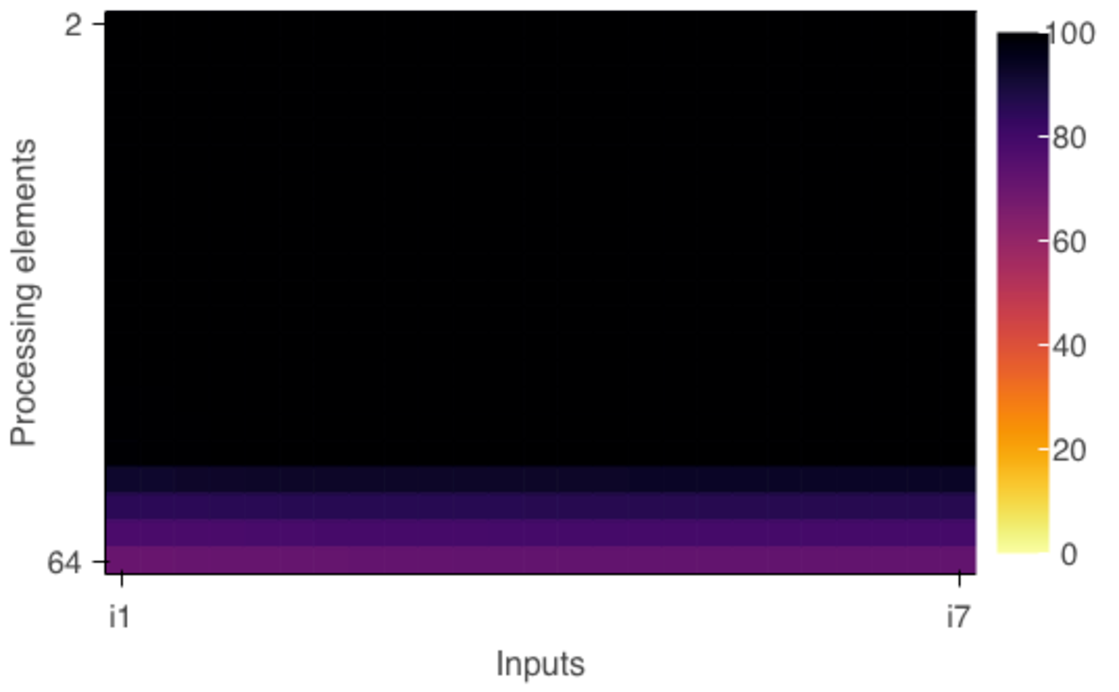
\includegraphics[width=\textwidth]{pascalanalyzer/figures/results/regionscomparison_r1.pdf}
		\caption{\centering}
		\label{fig:pv_regionscomparison_a}
	\end{subfigure}
	\begin{subfigure}[b]{0.45\textwidth}
		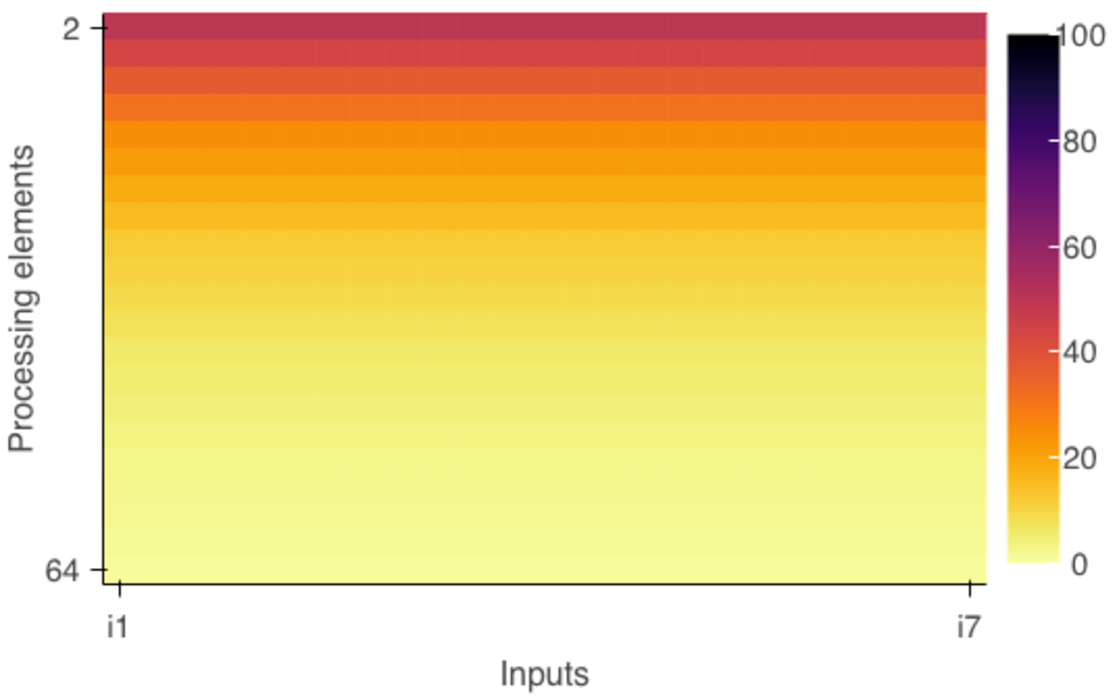
\includegraphics[width=\textwidth]{pascalanalyzer/figures/results/regionscomparison_r2.pdf}
		\caption{\centering}
		\label{fig:pv_regionscomparison_b}
	\end{subfigure}
	\begin{subfigure}[b]{0.45\textwidth}
		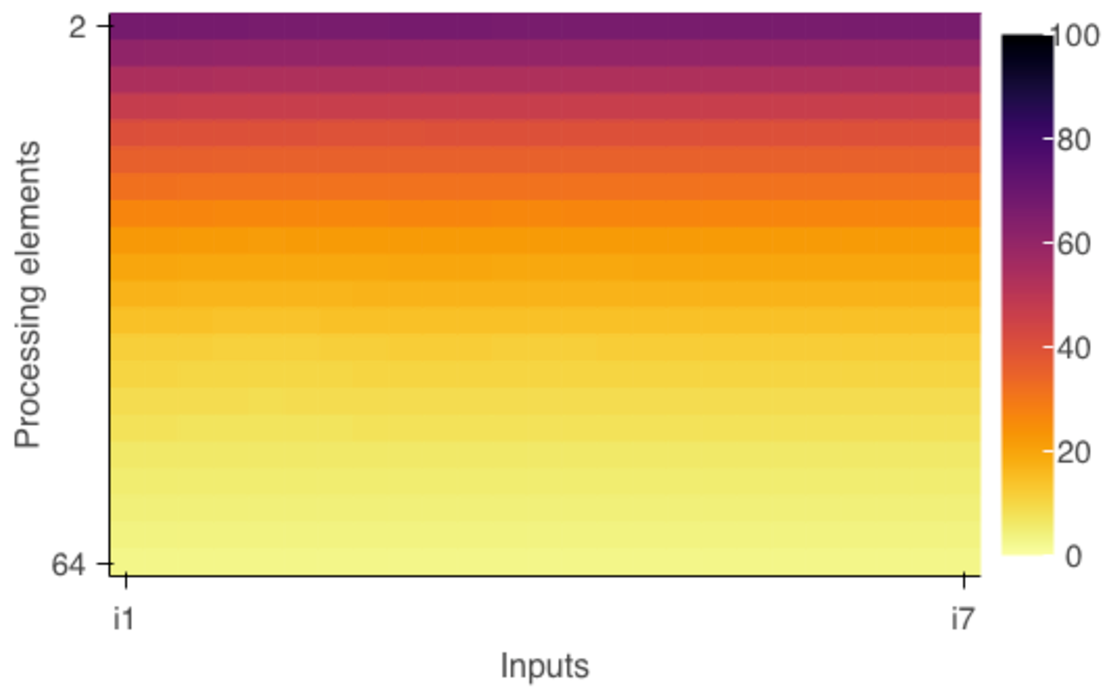
\includegraphics[width=\textwidth]{pascalanalyzer/figures/results/regionscomparison_whole.pdf}
		\caption{\centering}
		\label{fig:pv_regionscomparison_c}
	\end{subfigure}
	\caption{Efficiency diagrams and impact of inner regions on program scalability. (x-axis = inputs; y-axis = number of threads). (\textbf{a}) First region diagram. (\textbf{b}) Second region diagram. (\textbf{c}) Whole program~diagram.}
	\label{fig:pv_regionscomparison}
\end{figure}
\unskip
\begin{figure}[H]
	\begin{subfigure}[b]{0.45\textwidth}
		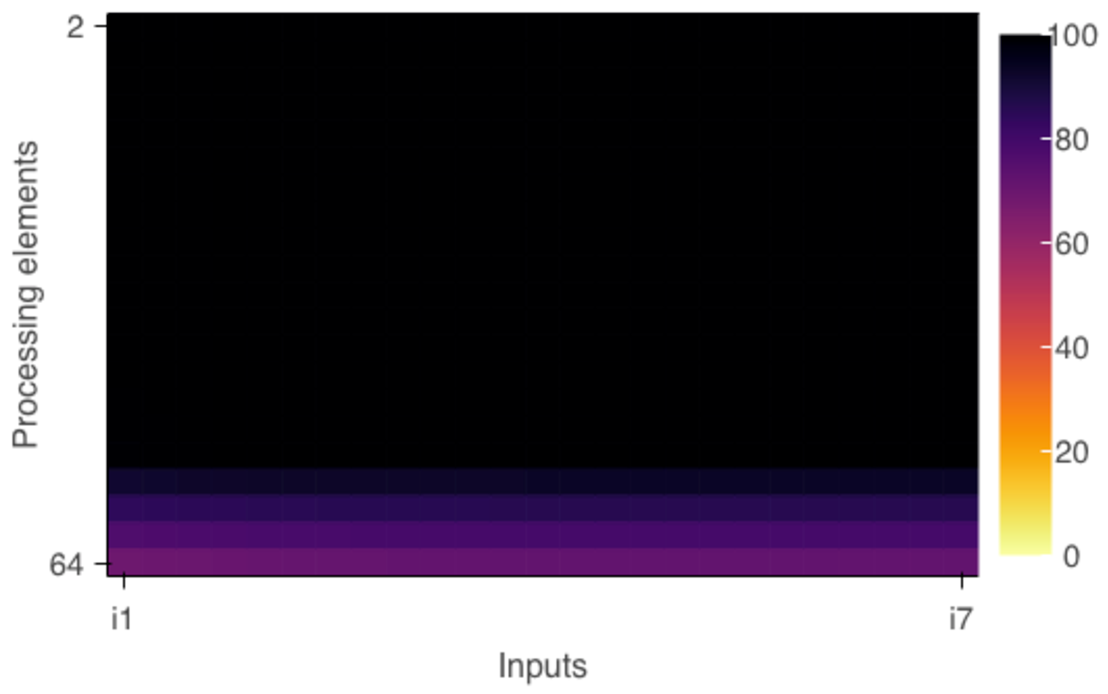
\includegraphics[width=\textwidth]{pascalanalyzer/figures/results/efficiency_rg_1.pdf}
		\caption{\centering}
		\label{fig:pv_regionscomparison_a_2}
	\end{subfigure}
	\begin{subfigure}[b]{0.45\textwidth}
		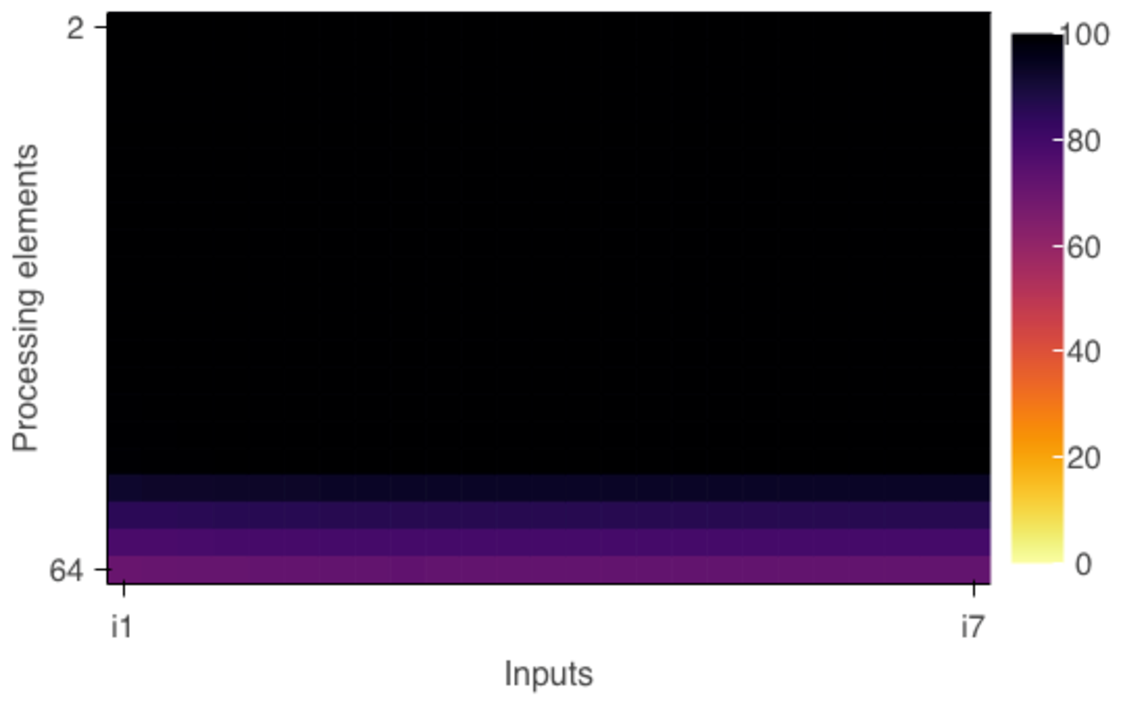
\includegraphics[width=\textwidth]{pascalanalyzer/figures/results/efficiency_rg_2.pdf}
		\caption{\centering}
		\label{fig:pv_regionscomparison_b_2}
	\end{subfigure}
	\begin{subfigure}[b]{0.45\textwidth}
		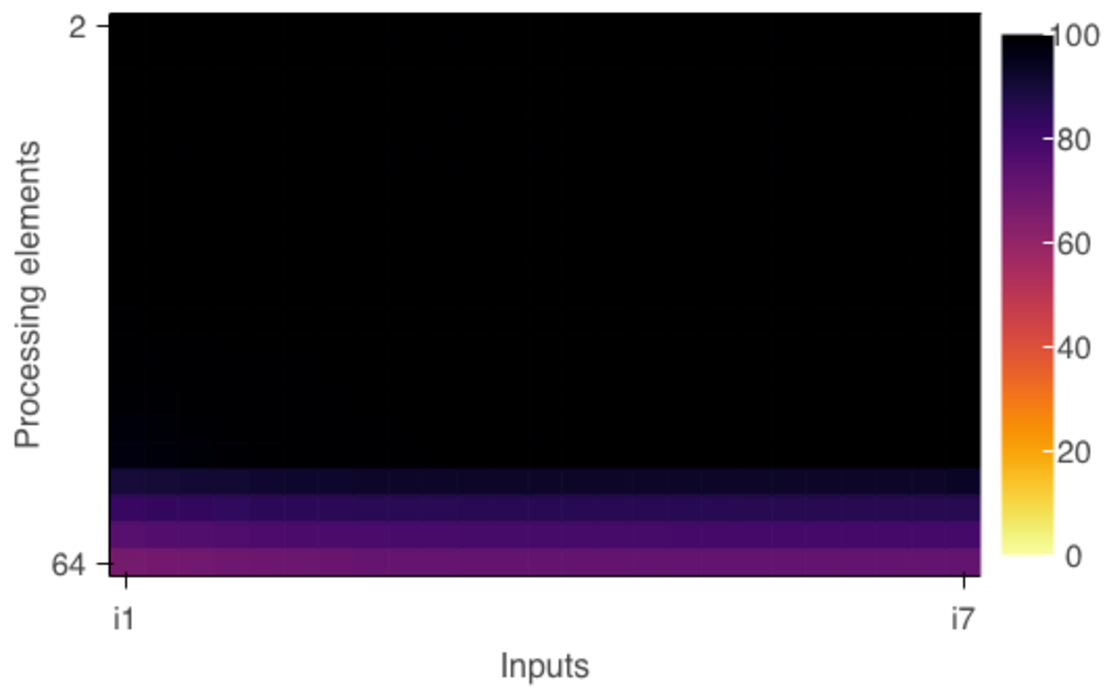
\includegraphics[width=\textwidth]{pascalanalyzer/figures/results/efficiency_rg_3.pdf}
		\caption{\centering}
		\label{fig:pv_regionscomparison_c_2}
	\end{subfigure}
	\caption{Efficiency diagrams after removing {\tt \#pragma~omp~crtical} clause. (x-axis = inputs; y-axis = number of threads). (\textbf{a}) First region diagram. (\textbf{b}) Second region diagram. (\textbf{c}) Whole program~diagram.}
	\label{fig:pv_regionscomparison_2}
\end{figure}
\unskip
\begin{figure}[H]
	\begin{subfigure}[b]{0.45\textwidth}
		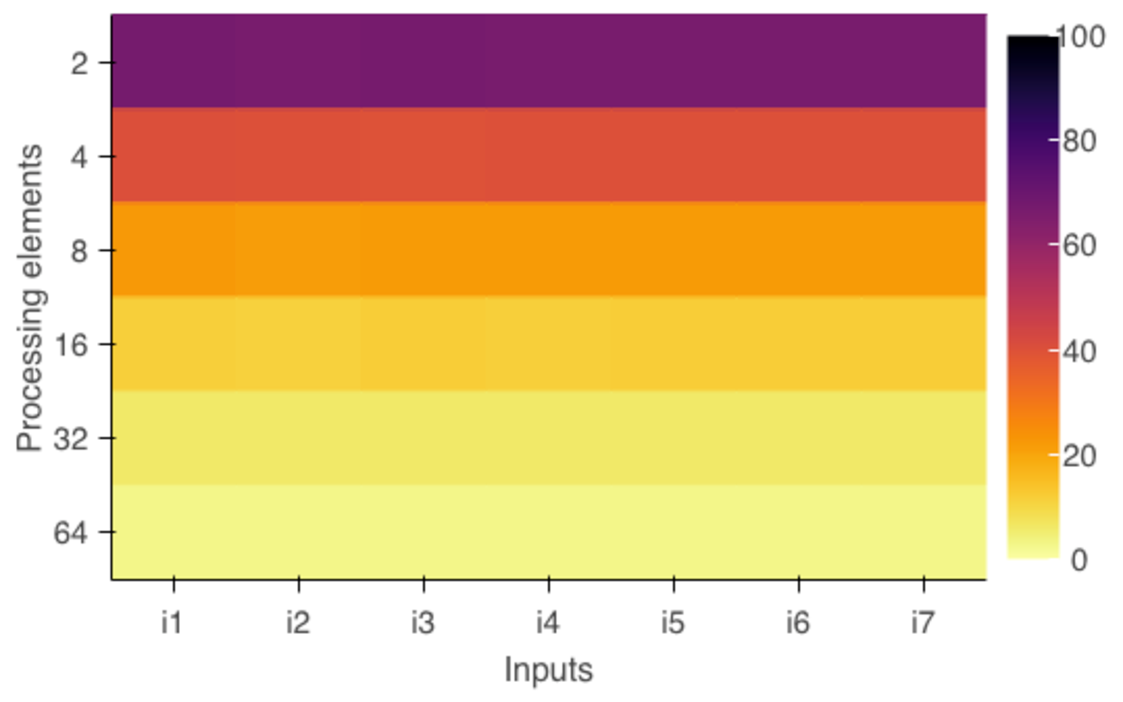
\includegraphics[width=\textwidth]{pascalanalyzer/figures/results/diagram_discretevalues.pdf}
		\caption{\centering}
		\label{fig:discretevalues}
	\end{subfigure}
	%
	\begin{subfigure}[b]{0.45\textwidth}
		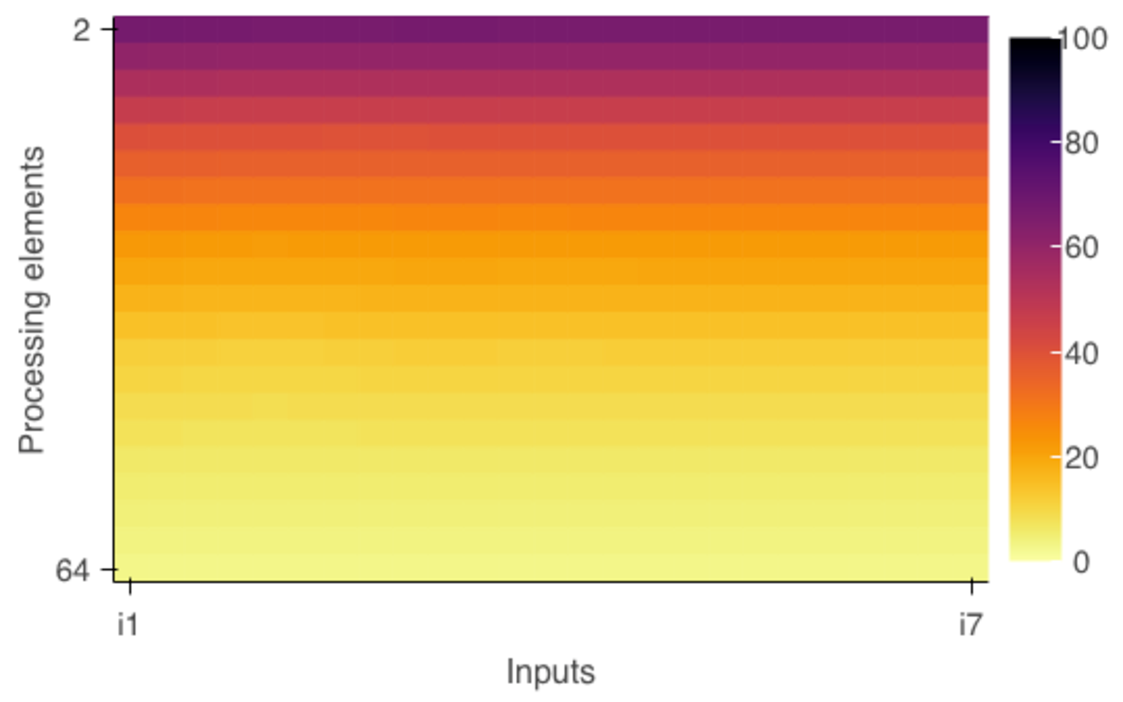
\includegraphics[width=\textwidth]{pascalanalyzer/figures/results/diagram_smoothedvalues.pdf}
		\caption{\centering}
		\label{fig:smoothedvalues}
	\end{subfigure}
	
	\caption{Visualization modes of diagrams provided by PaScal Viewer. (\textbf{a}) PaScal Viewer diagram on discrete mode. (\textbf{b}) PaScal Viewer diagram on smoothed mode.}
	\label{fig:visualizationmodes}
\end{figure}


%The analyzer allows that the result can be seen in tabular form, as shown in Table.~\ref{tab:regtable_dedup}. Using these tables, we can quickly generate figures that show the application's behavior from various points of view. In Figures \ref{fig:speedup_raytrace} and \ref{fig:speedup_openmc} we can observe the trend of the speedup with the number of cores and input.

%Figures \ref{fig:raytrace_en} and \ref{fig:openmc_en} present the energy variation with the number of cores.

\textls[-19]{Other analysis objectives not supported by PaScal Viewer, such as visualization of the speedup curve or energy consumption, can be supported by traditional plots. Figures~\ref{fig:speedup} and \ref{fig:energy}} present the charts rendered for analysis by Raytrace and OpenMC applications. In these figures, it is possible to observe that the program efficiency varies according to the increase in the number of threads and the execution of inputs with higher processing loads. From the diagrams in \cref{fig:efficiency_all}, it is possible to observe that the applications present different behaviors concerning their efficiency variations and their scalability capabilities. OpenMC maintains its efficiency almost constant. This pattern represents strong scalability and indicates that the program can maintain its efficiency level when it uses a larger number of threads and processing larger inputs. On the other hand, \cref{fig:efficiency_all}a demonstrates that Raytrace achieves higher efficiency values when processing larger inputs. However, it is also possible to observe that increasing the number of processing units fixing the input size will not improve or hold the efficiency value.
\begin{figure}[H]
	\begin{subfigure}[b]{0.45\textwidth}
		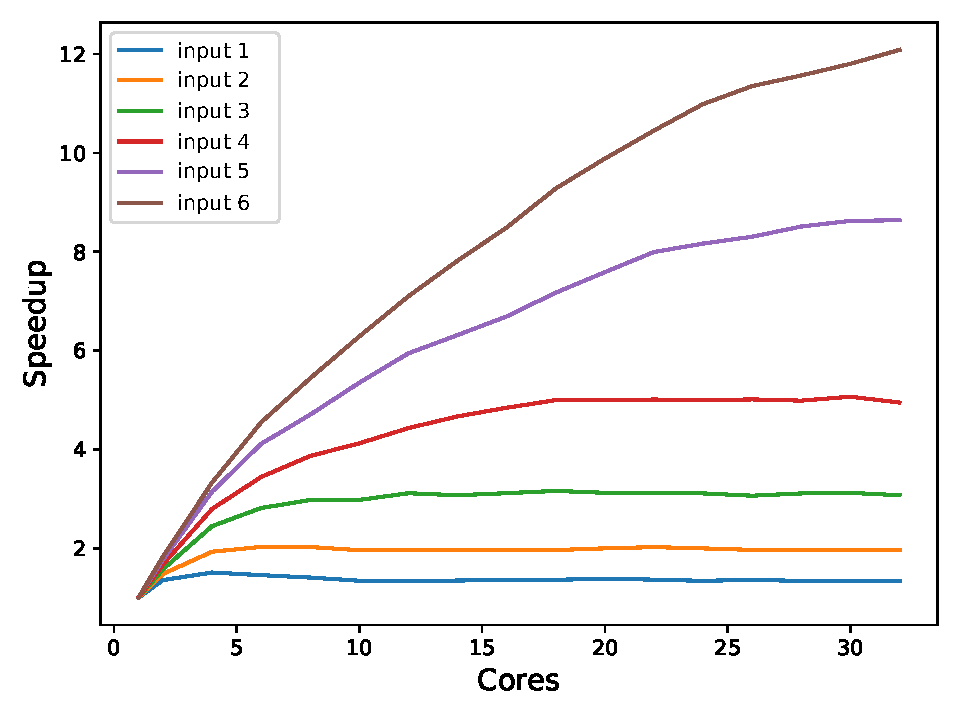
\includegraphics[width=\textwidth]{pascalanalyzer/figures/results/speedup_completo_rtview_2 (1).pdf}
		\caption{\centering}
		\label{fig:speedup_raytrace}
	\end{subfigure}
	%
	\begin{subfigure}[b]{0.45\textwidth}
		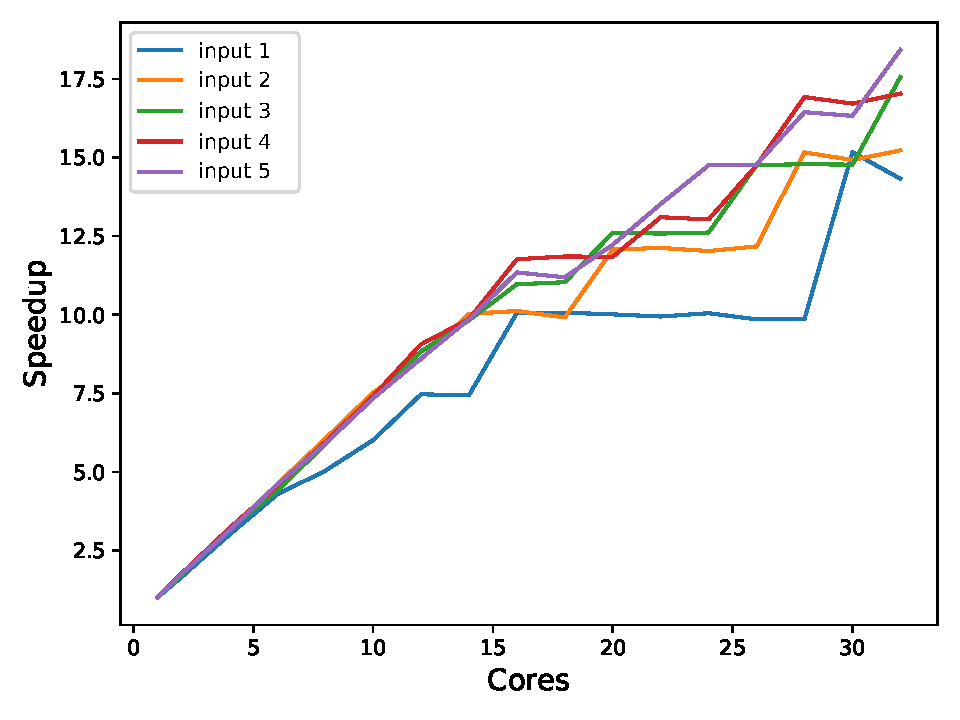
\includegraphics[width=\textwidth]{pascalanalyzer/figures/results/speedup_completo_openmc_kernel_novo (1).pdf}
		\caption{\centering}
		\label{fig:speedup_openmc}
	\end{subfigure}
	\caption{\textls[-30]{Speedup of the applications for several input sizes. (\textbf{a}) Raytrace speedup. (\textbf{b}) OpenMC speedup. }}
	\label{fig:speedup}
\end{figure}
\unskip
\begin{figure}[H]
	\begin{subfigure}[b]{0.46\textwidth}
		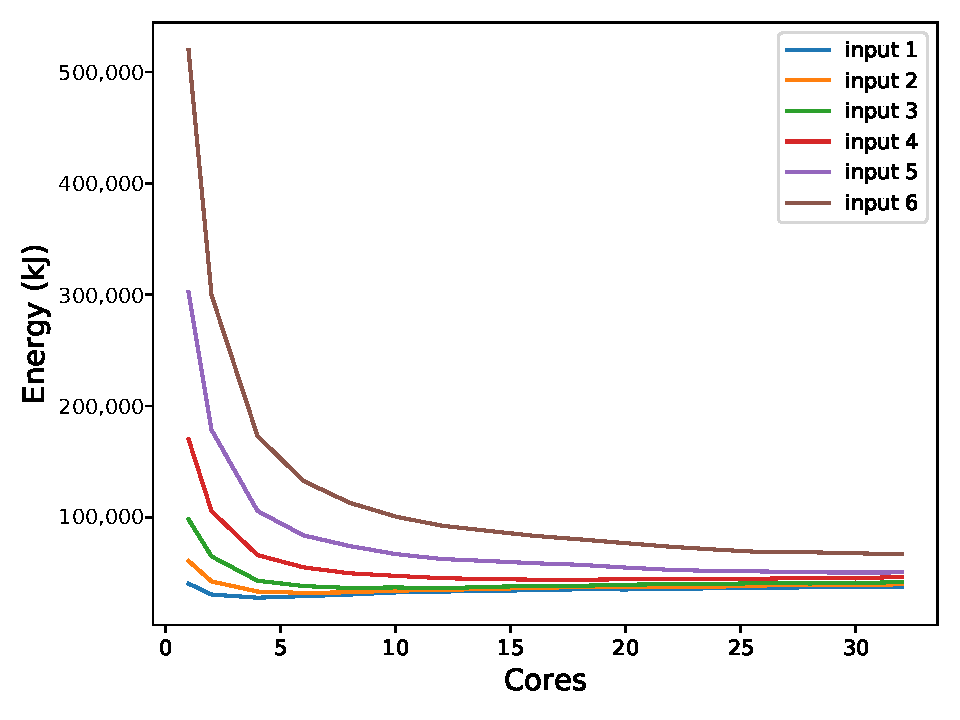
\includegraphics[width=\textwidth]{pascalanalyzer/figures/results/energy_completo_rtview_2 (1).pdf}
		\caption{\centering}
		\label{fig:raytrace_en}
	\end{subfigure}
	%
	\begin{subfigure}[b]{0.46\textwidth}
		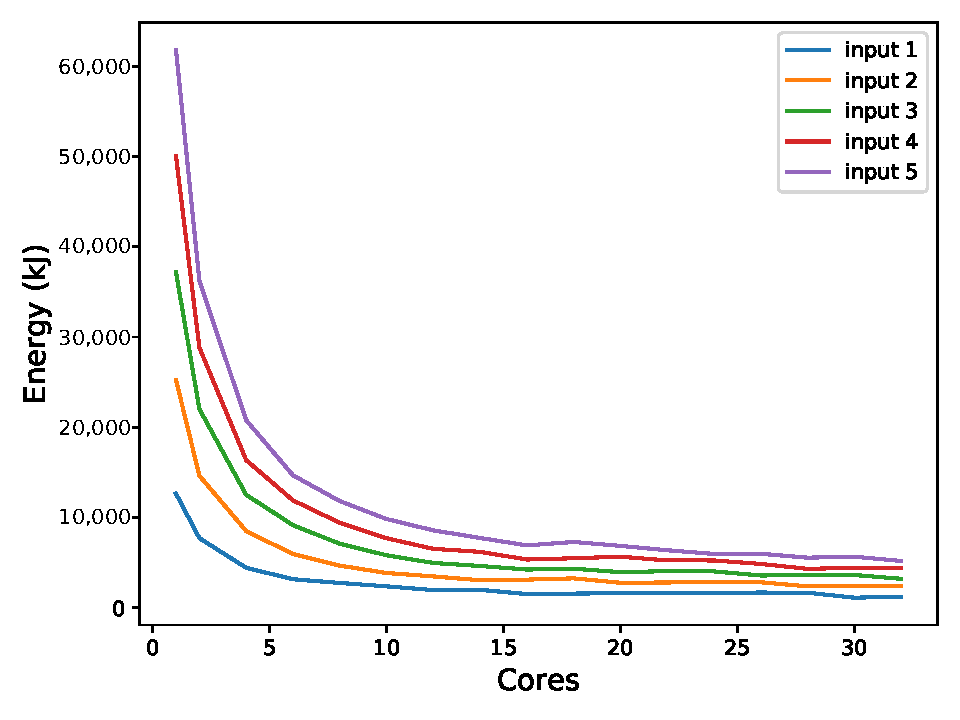
\includegraphics[width=\textwidth]{pascalanalyzer/figures/results/energy_completo_openmc_kernel_novo (1).pdf}
		\caption{\centering}
		\label{fig:openmc_en}
	\end{subfigure}
	
	\caption{Energy consumption identified in the execution of applications while varying the number of cores for several input sizes.
		%MDPI: Please add commas to numbers to indicate thousand on the Oy axis of the figures, e.g. 20,000 30,000 40,000.
		(\textbf{a}) Raytrace energy consumption. (\textbf{b}) OpenMC energy consumption.}
	\label{fig:energy}
\end{figure}
\unskip
%Furthermore, using an external graphical interface module, we can load the .json file and intuitively visualize the program's scalability showing the efficiency. The efficiency pinpoint how efficiently a program can take advantage of increasing processing elements on a parallel system. It is defined as the ratio of speedup to the number of processors.
%For example, Figure \ref{fig:efficiency_all} shows examples of graphics generated for the same applications as above. In these figures, it is possible to observe that the program efficiency varies according to the increase in the number of threads and the execution of inputs with higher processing loads. From the Figure \ref{fig:efficiency_raytrace} we can see that as we increase the input size, the efficiency increases while slowly decreasing when the number of cores grows, indicating a tendency for a scalable program. In the second Figure \ref{fig:efficiency_openmc} the efficiency is practically constant while varying the number of cores and the input indicating a strong scalable program.
\begin{figure}[H]
	\begin{subfigure}[b]{0.46\textwidth}
		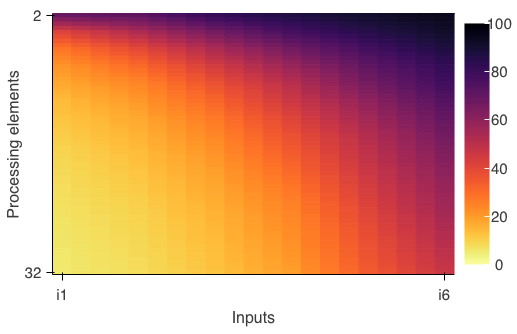
\includegraphics[width=\textwidth]{pascalanalyzer/figures/results/efficiency_raytrace.png}
		\caption{\centering}
		\label{fig:efficiency_raytrace}
	\end{subfigure}
	\begin{subfigure}[b]{0.46\textwidth}
		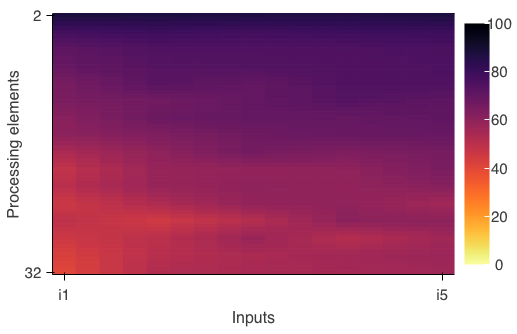
\includegraphics[width=\textwidth]{pascalanalyzer/figures/results/efficiency_openmc.png}
		\caption{\centering}
		\label{fig:efficiency_openmc}
	\end{subfigure}
	
	\caption{Efficiency diagram varying the input size and the number of cores. The color bar indicates the efficiency value in percentage. (\textbf{a}) Raytrace efficiency diagram. (\textbf{b}) OpenMC efficiency diagram.}
	\label{fig:efficiency_all}
\end{figure}

The input values shown in Figures~\ref{fig:speedup}--\ref{fig:efficiency_all} indicate different data sets for processing. For example, the ``input 2'' represents a load that will require sequential processing with runtime twice as long as ``input 1''. Likewise, the ``input 3'' represents a load that will require sequential processing with runtime twice as long as ``input 2'', and so on.

Even if the analyzer does not display graphics natively, analysis aimed at observing scalability and energy consumption of applications depends on precise measurements, reinforcing the advantage of the analyzer proposed in this work.

% \begin{figure}[H]
% \centering
% 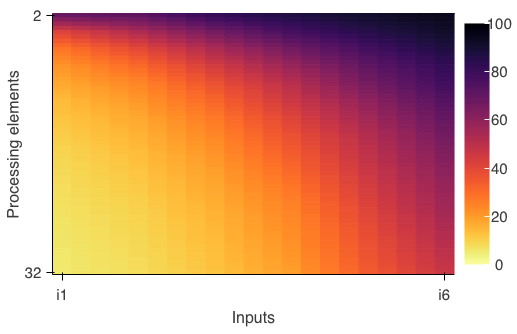
\includegraphics[width=\linewidth]{pascalanalyzer/figures/results/efficiency_raytrace.png}
% \caption{Efficiency for Raytrace}
% \label{fig:efficiency_raytrace}
% \end{figure}

% \begin{figure}[H]
% \centering
% 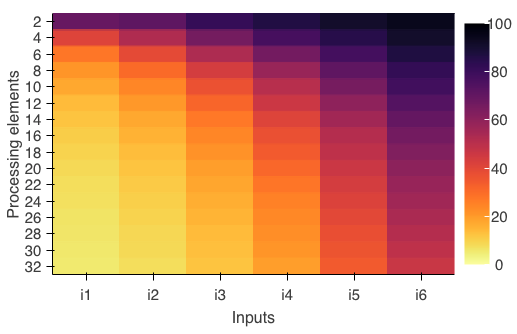
\includegraphics[width=\linewidth]{pascalanalyzer/figures/results/efficiency_raytrace_detailed.png}
% \caption{Efficiency for Raytrace}
% \label{fig:efficiency_raytrace_detailed}
% \end{figure}

% \begin{figure}[H]
% \centering
% 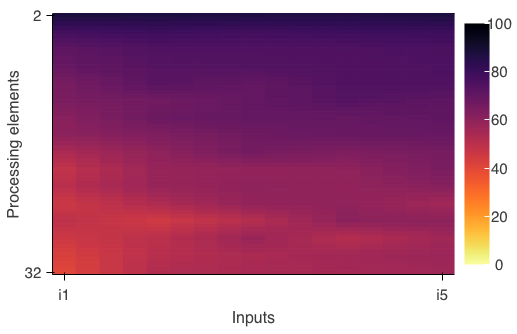
\includegraphics[width=\linewidth]{pascalanalyzer/figures/results/efficiency_openmc.png}
% \caption{Efficiency for OpenMC}
% \label{fig:efficiency_openmc}
% \end{figure}

% \begin{figure}[H]
% \centering
% 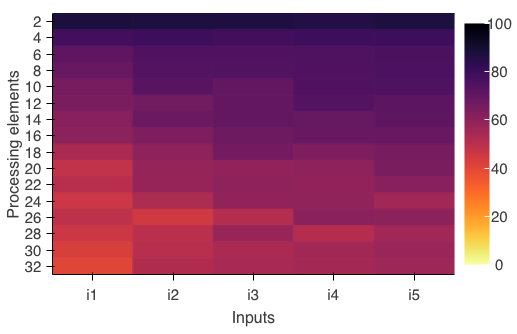
\includegraphics[width=\linewidth]{pascalanalyzer/figures/results/efficiency_openmc_detailed.png}
% \caption{Efficiency for OpenMC}
% \label{fig:efficiency_openmc_detailed}
% \end{figure}
\subsection{Fingerprint Tool validation}

In this subsection, we first show the comparison between our tool and others already established, as well as the clustering process.

\subsubsection{ACCURACY COMPARISON}

% \begin{table*}[h]
% \centering
% \caption{Average}
% \begin{tabular}{|c|c|c|c|c|c|c|}
% \hline
% Counter                                 & Pined values & Linux API   & PAPI      & PAPI Python & Perf tool   & MyPerf      \\ \hline
% INSTRUCTIONS\_RETIRED                  & 226990030    & 227000691   & 227000620 & 225901249   & 227000572   & 227000650   \\ \hline
% BRANCH\_INSTRUCTIONS\_RETIRED          & 9240000      & 9250617     & 9250566   & 9239617     & 9250552     & 9250501     \\ \hline
% BR\_INST\_RETIRED:CONDITIONAL          & 8220000      & 8220000     & 8220000   & 8209717     & 8220000     & 8220000     \\ \hline
% MEM\_UOP\_RETIRED:ANY\_LOADS           &              & 2484182672  &           &             & 2484383940  & 2484155029  \\ \hline
% MEM\_UOP\_RETIRED:ANY\_STORES          &              & 189962002   &           &             & 189961539   & 189961321   \\ \hline
% UOPS\_RETIRED:ANY                      &              & 12291082129 &           &             & 12290811038 & 12290901997 \\ \hline
% PARTIAL\_RAT\_STALLS:MUL\_SINGLE\_UOP  &              & 600878      &           &             & 600151      & 600330      \\ \hline
% ARITH:FPU\_DIV                         &              & 5801446     &           &             & 5801000     & 5800977     \\ \hline
% FP\_COMP\_OPS\_EXE:X87                 &              & 48785528    &           &             & 48784834    & 48786021    \\ \hline
% INST\_RETIRED:X87                      &              & 17200008    &           &             & 17200008    & 17200007    \\ \hline
% FP\_COMP\_OPS\_EXE:SSE\_SCALAR\_DOUBLE &              & 5401694     &           &             & 5401842     & 5401679     \\ \hline
% \end{tabular}
% \label{tab:mean}
% \end{table*}

% \begin{table*}[h]
% \centering
% \caption{Standard deviation}
% \begin{tabular}{|c|c|c|c|c|c|}
% \hline
% Counter                                    & Linux API & PAPI & PAPI Python & Perf tool & MyPerf \\ \hline
% INSTRUCTIONS\_RETIRED                  & 396       & 133  & 337763      & 110       & 175    \\ \hline
% BRANCH\_INSTRUCTIONS\_RETIRED          & 297       & 208  & 8485        & 379       & 91     \\ \hline
% BR\_INST\_RETIRED:CONDITIONAL          & 0         & 0    & 3383        & 0         & 0      \\ \hline
% MEM\_UOP\_RETIRED:ANY\_LOADS           & 37399     &      &             & 39217     & 38953  \\ \hline
% MEM\_UOP\_RETIRED:ANY\_STORES          & 1513      &      &             & 1035      & 687    \\ \hline
% UOPS\_RETIRED:ANY                      & 345246    &      &             & 335832    & 333298 \\ \hline
% PARTIAL\_RAT\_STALLS:MUL\_SINGLE\_UOP  & 1222      &      &             & 252       & 521    \\ \hline
% ARITH:FPU\_DIV                         & 1760      &      &             & 1621      & 1544   \\ \hline
% FP\_COMP\_OPS\_EXE:X87                 & 1283      &      &             & 1920      & 3311   \\ \hline
% INST\_RETIRED:X87                      & 4         &      &             & 4         & 3      \\ \hline
% FP\_COMP\_OPS\_EXE:SSE\_SCALAR\_DOUBLE & 1547      &      &             & 3259      & 2097   \\ \hline
% \end{tabular}
% \label{tab:std}
% \end{table*}

\begin{table}[H]
	\centering
	\caption{Comparison}
	\resizebox{\textwidth}{!}{%
		\begin{tabular}{llllllllll}
			\hline
			\multicolumn{6}{l|}{\textbf{Average*$10^{-6}$}} & \multicolumn{4}{l}{\textbf{Standard deviation}}\\ \hline
			\textbf{Counters} & \begin{tabular}{l}\textbf{Pined} \\ \textbf{values}\end{tabular} & \begin{tabular}{l}\textbf{Linux} \\ \textbf{API}\end{tabular} & \textbf{PAPI} & \begin{tabular}{l}\textbf{PAPI} \\ \textbf{Python}\end{tabular} & \textbf{MyPerf}  & \begin{tabular}{|l}\textbf{Linux} \\ \textbf{API}\end{tabular} & \textbf{PAPI} & \begin{tabular}{l}\textbf{PAPI} \\ \textbf{Python}\end{tabular} & \textbf{MyPerf} \\ \hline
			INSTRUCTIONS\_RETIRED                  & 226.99       & 227       & 227  & 225.9       & 227     & 396       & 133  & 337763      & 175    \\
			BRANCH\_INSTRUCTIONS\_RETIRED          & 9.24         & 9.25      & 9.25 & 9.24        & 9.25    & 297       & 208  & 8485        & 91     \\
			BR\_INST\_RETIRED:CONDITIONAL          & 8.22         & 8.22      & 8.22 & 8.21        & 8.22    & 0         & 0    & 3383        & 0      \\
			MEM\_UOP\_RETIRED:ANY\_LOADS           &              & 2484.18   &      &             & 2484.16 & 37399     &      &             & 38953  \\
			MEM\_UOP\_RETIRED:ANY\_STORES          &              & 189.96    &      &             & 189.96  & 1513      &      &             & 687    \\
			UOPS\_RETIRED:ANY                      &              & 12291.08  &      &             & 12290.9 & 345246    &      &             & 333298 \\
			PARTIAL\_RAT\_STALLS:MUL\_SINGLE\_UOP  &              & 0.6       &      &             & 0.6     & 1222      &      &             & 521    \\
			ARITH:FPU\_DIV                         &              & 5.8       &      &             & 5.8     & 1760      &      &             & 1544   \\
			FP\_COMP\_OPS\_EXE:X87                 &              & 48.79     &      &             & 48.79   & 1283      &      &             & 3311   \\
			INST\_RETIRED:X87                      &              & 17.2      &      &             & 17.2    & 4         &      &             & 3      \\
			FP\_COMP\_OPS\_EXE:SSE\_SCALAR\_DOUBLE &              & 5.4       &      &             & 5.4     & 1547      &      &             & 2097   \\ \hline
		\end{tabular}
	}
	\label{tab:counters}
\end{table}

To validate the tool, we compared the results of the counters obtained with different APIs. 
We used the hand-crafted assembly benchmark from \cite{Weaver2013Non-determinismImplementations}, designed to test determinism and accuracy of PMUs.
We compared the values obtained from the Linux API, PAPI on C and PAPI on Python. 
The events used for this comparison were instructions retired, branch instructions, memory read, memory load, and arithmetic operations.
We ran the benchmark 30 times and calculated the mean and standard deviation as shown in table \ref{tab:counters}. Some events could not be measured using PAPI because the tool does not accept raw events and there are no equivalent events.

Since the benchmark was hand-crafted with assembly, we know exactly the value for some counter events. 
For this reason, the number of instructions, branch instructions, and conditional branch are pin. However, some other events are architecture-specific and there is no pined value. 
In the latter case, we can still compare to the Linux API, which should be closest to the reality.

The differences using the Linux low-level API, PAPI, and our tool are negligible (the average percentage distance is less than 0.01\% in all the cases). 
As expected, PAPI on Python had the largest difference (with an average distance of 0.25\%) mainly due to an unsynchronized start that resulted in the loss of some instructions at the beginning of the execution. 
This can be an important problem if the application contains a small number of instructions.

The standard deviation of the 30 executions shows that our tool has the smallest variation on a run-to-run on most events. On the contrary, PAPI on Python shows a big variation compared to the others.

\subsubsection{CLUSTERING}

To cluster applications first we need to have a way to compare two programs, for that we define a new variable that tries to compute a fingerprint to the program, this variable has to look similar when we execute the same program with different conditions and inputs. Thinking in the simplest model of a program as a Turing machine as everything can be done with a tap of memory and set of rules we empirically define the variable input size as described on the equation \ref{eq:input_size}. On real computers this is not too far from reality, most of the computations and input and output operations somehow pass through the memory, so analyzing the relationship of the total number of instructions and memory instructions can give us a good fingerprint.

\begin{equation}
	I_{sz} = \frac{I}{I_{m}} \\
	\label{eq:input_size}
\end{equation}

Where $I_{sz}$ we called input size, $I$ the number of instructions executed, $I_m$ number of memory instructions execute. We observe that this variable demonstrate to have the proprieties that we are looking for, produce similar results to the same program with different input size, and environment. This can be used to identify programs but also to see the similarities between different applications.

To compute the distance between two programs we use the Canberra metric \cite{Jurman2009CanberraLists}, described on the equation \ref{eq:canberra}.

\begin{equation}
	d(p,q)= \sum_{i=1}^{n}{\frac{|p_i-q_i|}{|p_i|+|q_i|}}
	\label{eq:canberra}
\end{equation}

Where $p$ and $q$ are n-dimensional vectors.

We compute the input size for all 30 applications of the Polybench with 3 different inputs. Running each program 15 times, with a sampling rate of 0.01 seconds collecting the total number of instruction, number of loads and write instructions, number of floating point operations, besides some software counters. After applying the post-processing to the data collected we compute the input size and perform a Hierarchical clustering using the linkage method of Ward \cite{Murtagh2011WardsAlgorithm}, that minimizes the total within-cluster variance. The results of the clustering can be seen on the figure \ref{fig:sping_force_is} and on the dendrogram on figure \ref{fig:dendograma_input_size}.

%The exact HPCs was:
%PERF_COUNT_HW_INSTRUCTIONS,
%MEM_UOPS_RETIRED:ALL_LOADS,
%MEM_UOPS_RETIRED:ALL_STORES,
%FP_ARITH_INST_RETIRED:SCALAR

\begin{figure*}[h]
	\centering
	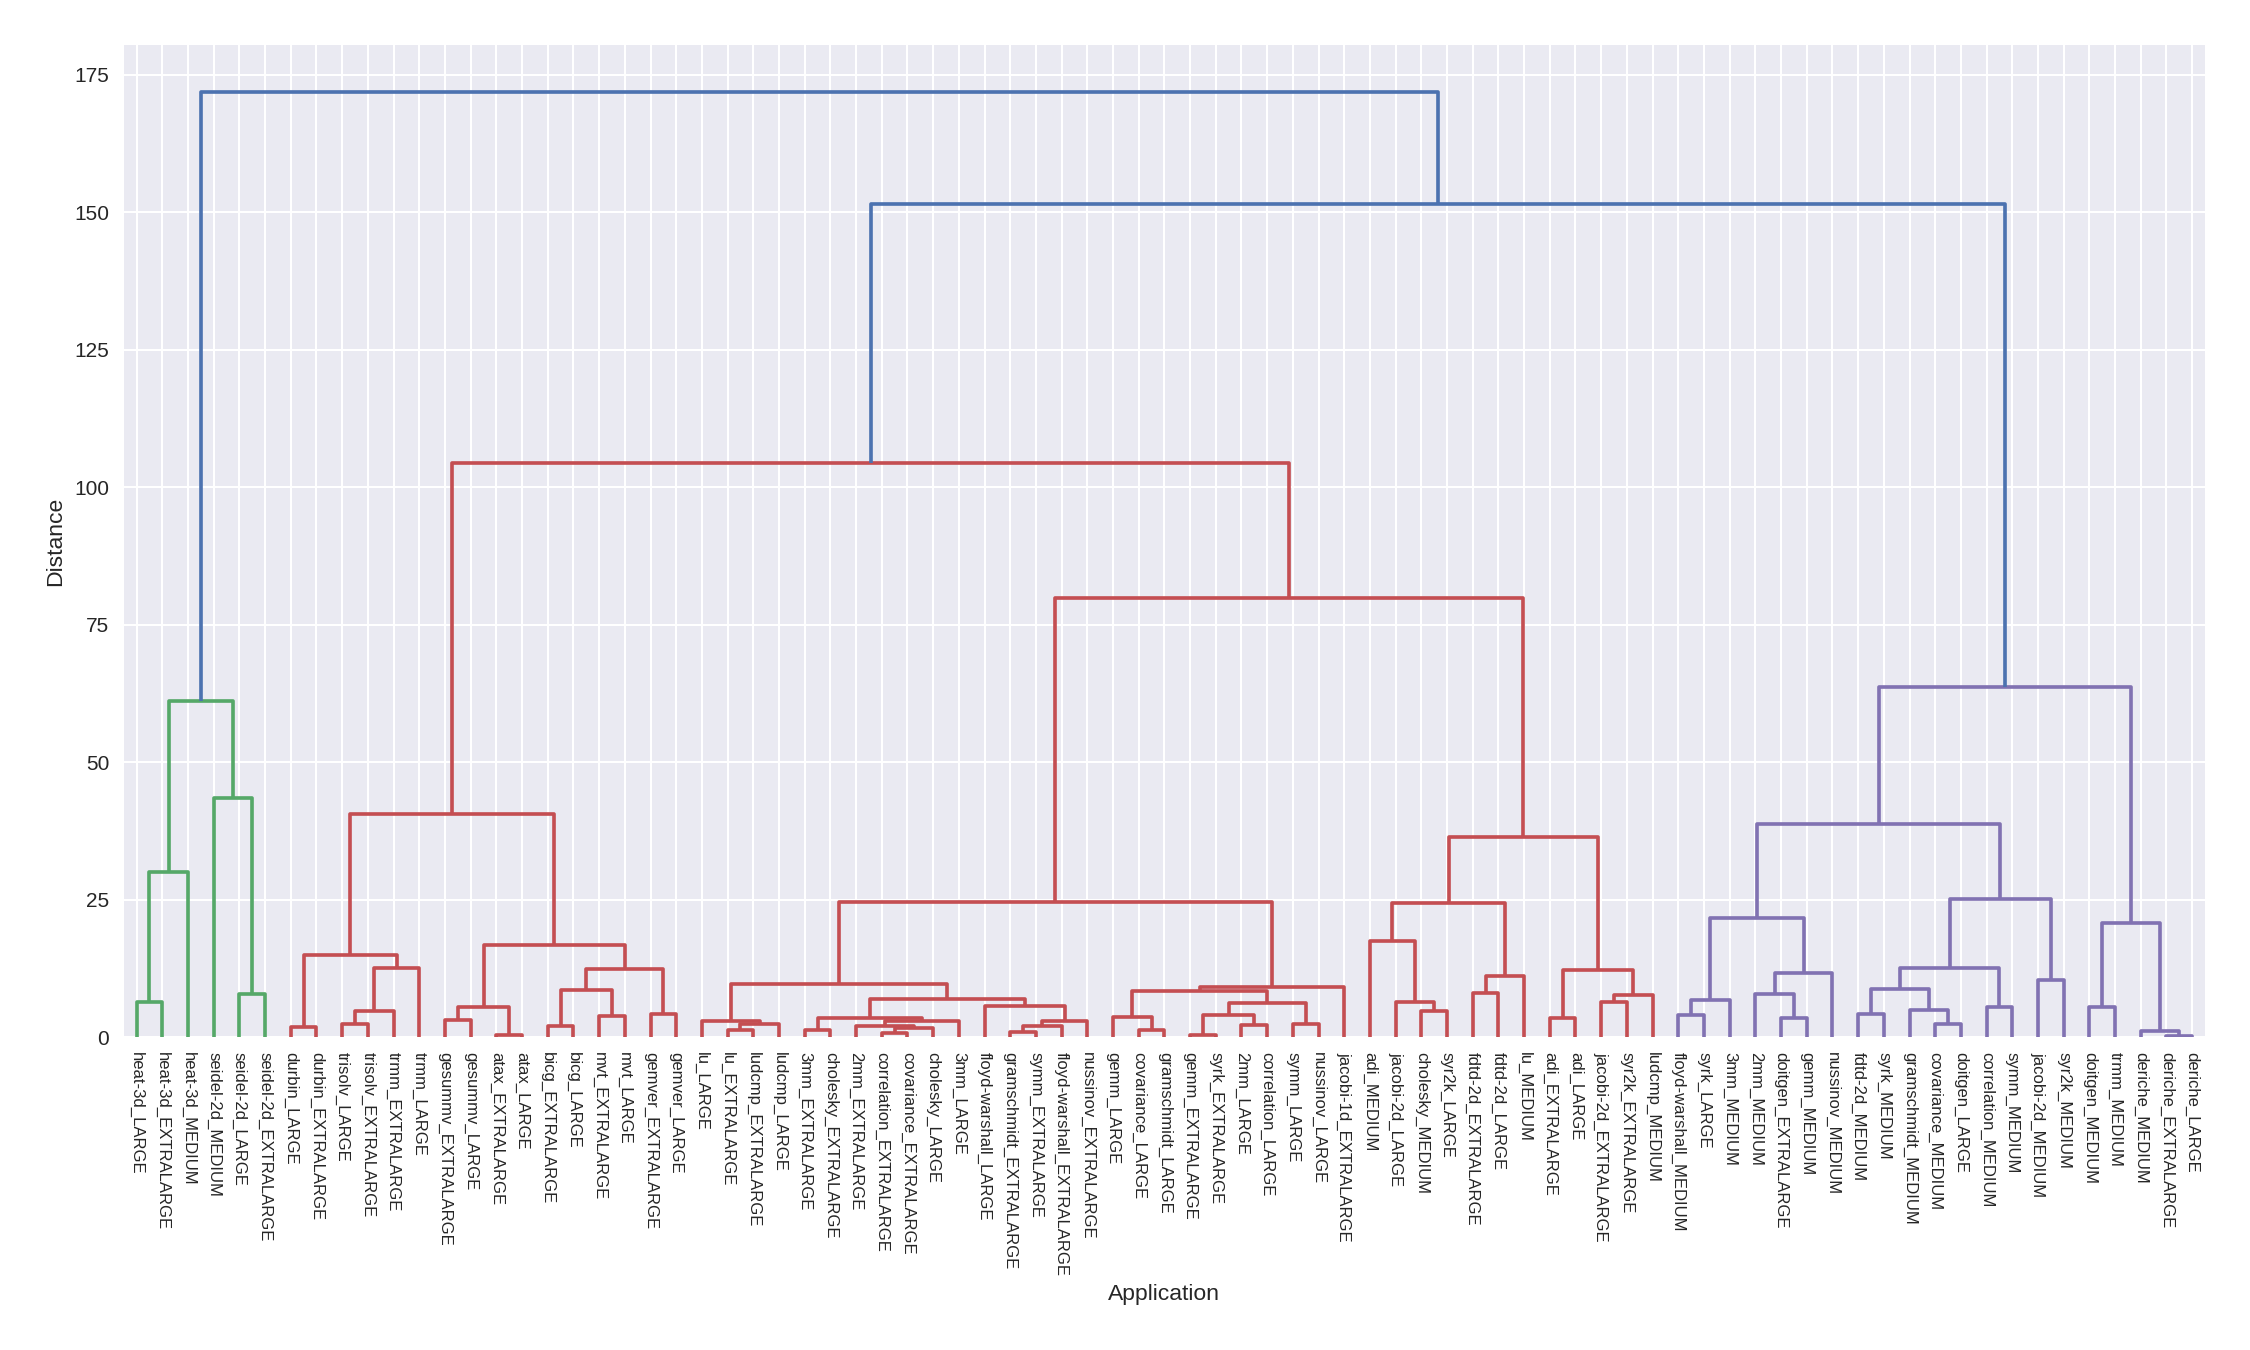
\includegraphics[width=\textwidth]{fingerprint/figures/dendograma_input_size.png}
	\caption{Dendrogram}
	\label{fig:dendograma_input_size}
\end{figure*}

From this dendrogram, we can have an idea of how close two applications are. We choose the number of clusters that maximize the number of hits of the same program with different input sizes on the same cluster, in this case, was 5 clusters.

It was observed that as input size grows the program behavior tends to a specific curve, but for small input sizes some have variation, so in some cases, the same program has been classified in more than one cluster. This can also happen if specific parts of the program are triggered with specific inputs, in which case it will also belong to more than one cluster.

In order to have an overall classification of each program, we can pick up the frequency in which each appeared in the clusters and classified it in the cluster in which it appeared more often. In this case, the clusters are:

\begin{itemize}
	\item Cluster 1: 2mm, 3mm, cholesky, correlation, covariance, floyd-warshall, gemm, gramschmidt, lu, ludcmp, nussinov, symm
	
	\item Cluster 2: deriche, doitgen, syrk
	
	\item Cluster 3: adi, fdtd-2d, jacobi-2d, syr2k
	
	\item Cluster 4: atax, bicg, durbin, gemver, gesummv, mvt, trisolv, trmm
	
	\item Cluster 5: heat-3d, seidel-2d
\end{itemize}

On the figure, \ref{fig:sping_force_is} we display the clusters using the spring force algorithm where each program with a specific input is a node and the edge weight is the Canberra distance. To a better visualization, the name of the inputs was replaced by numbers, the EXTRALARGE is 3, LARGE 2 and MEDIUM 1. 

\begin{figure}[H]
	\centering
	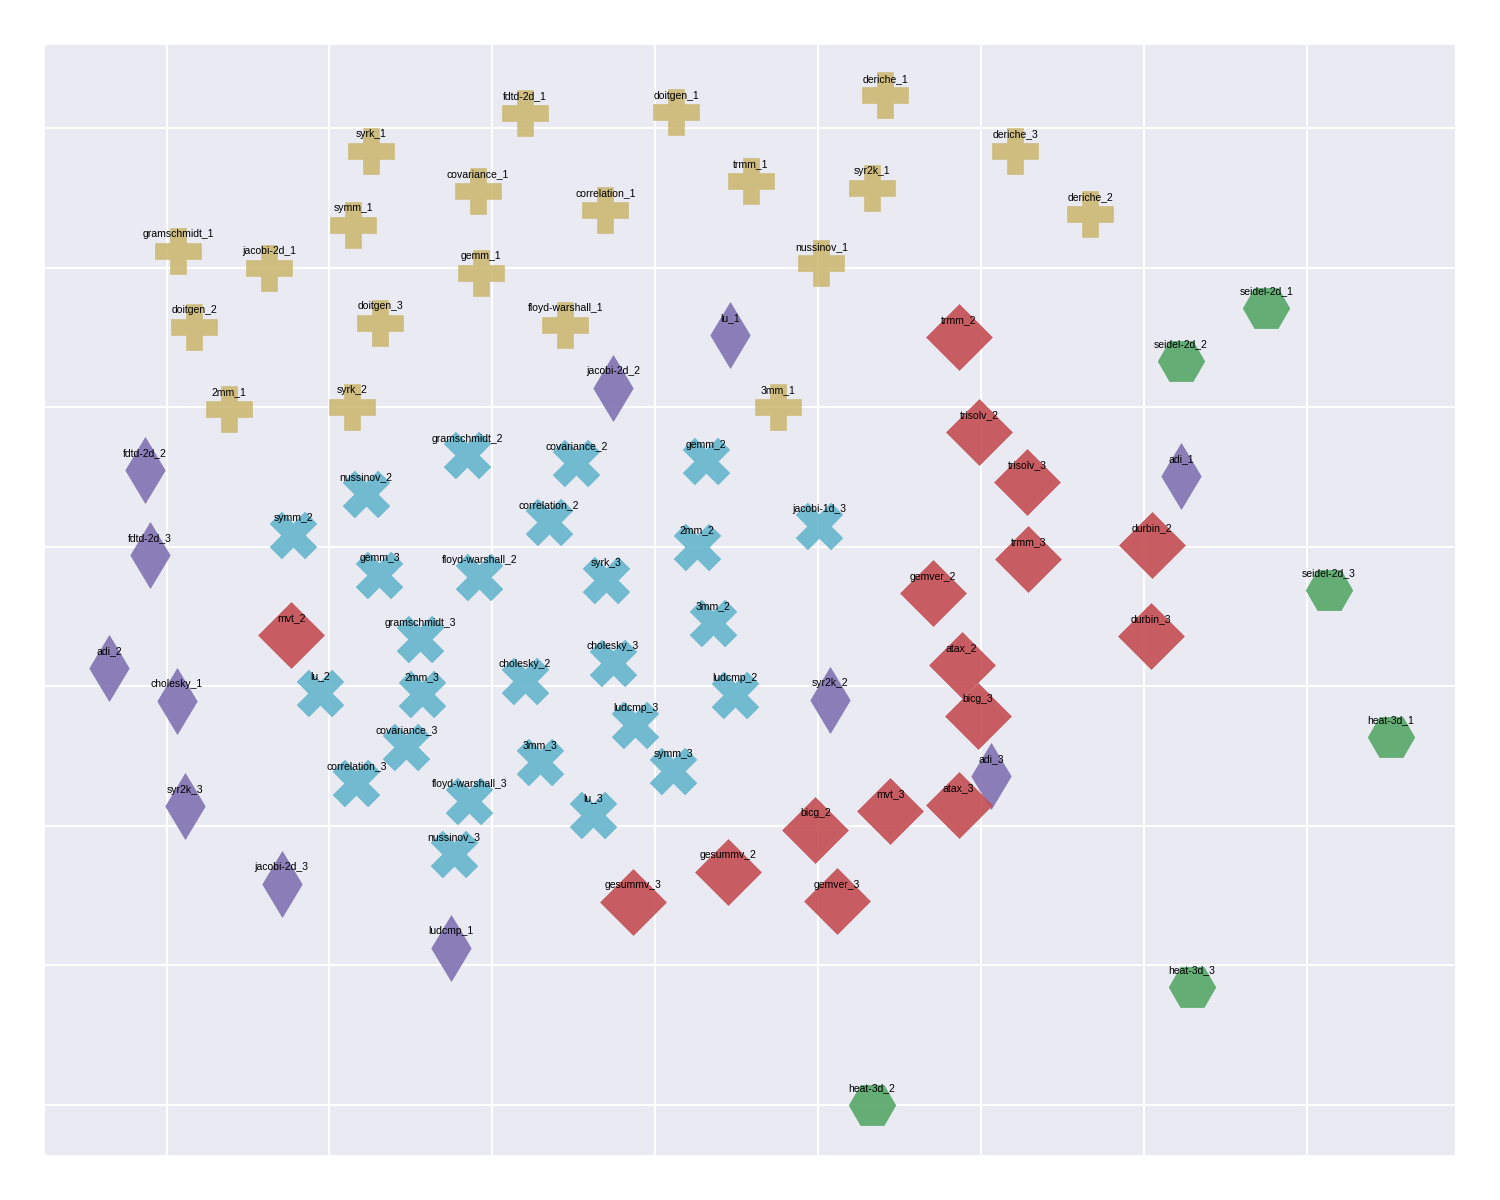
\includegraphics[width=\textwidth]{fingerprint/figures/graph_input_size.png}
	\caption{Spring force of Canberra distance}
	\label{fig:sping_force_is}
\end{figure}

The figure above shows a different way to observe in a reduced space the distance between clusters and applications and how they are organized. From this graph, we see that clustering it's well partitioned and we can clearly separate each cluster. It is also interesting to note that the applications of the cluster formed by the circle symbol are more separated, which may indicate that they were classified in this way because they did not fit into any other cluster.

% \begin{figure*}[t]
%     \begin{subfigure}{\textwidth}
%         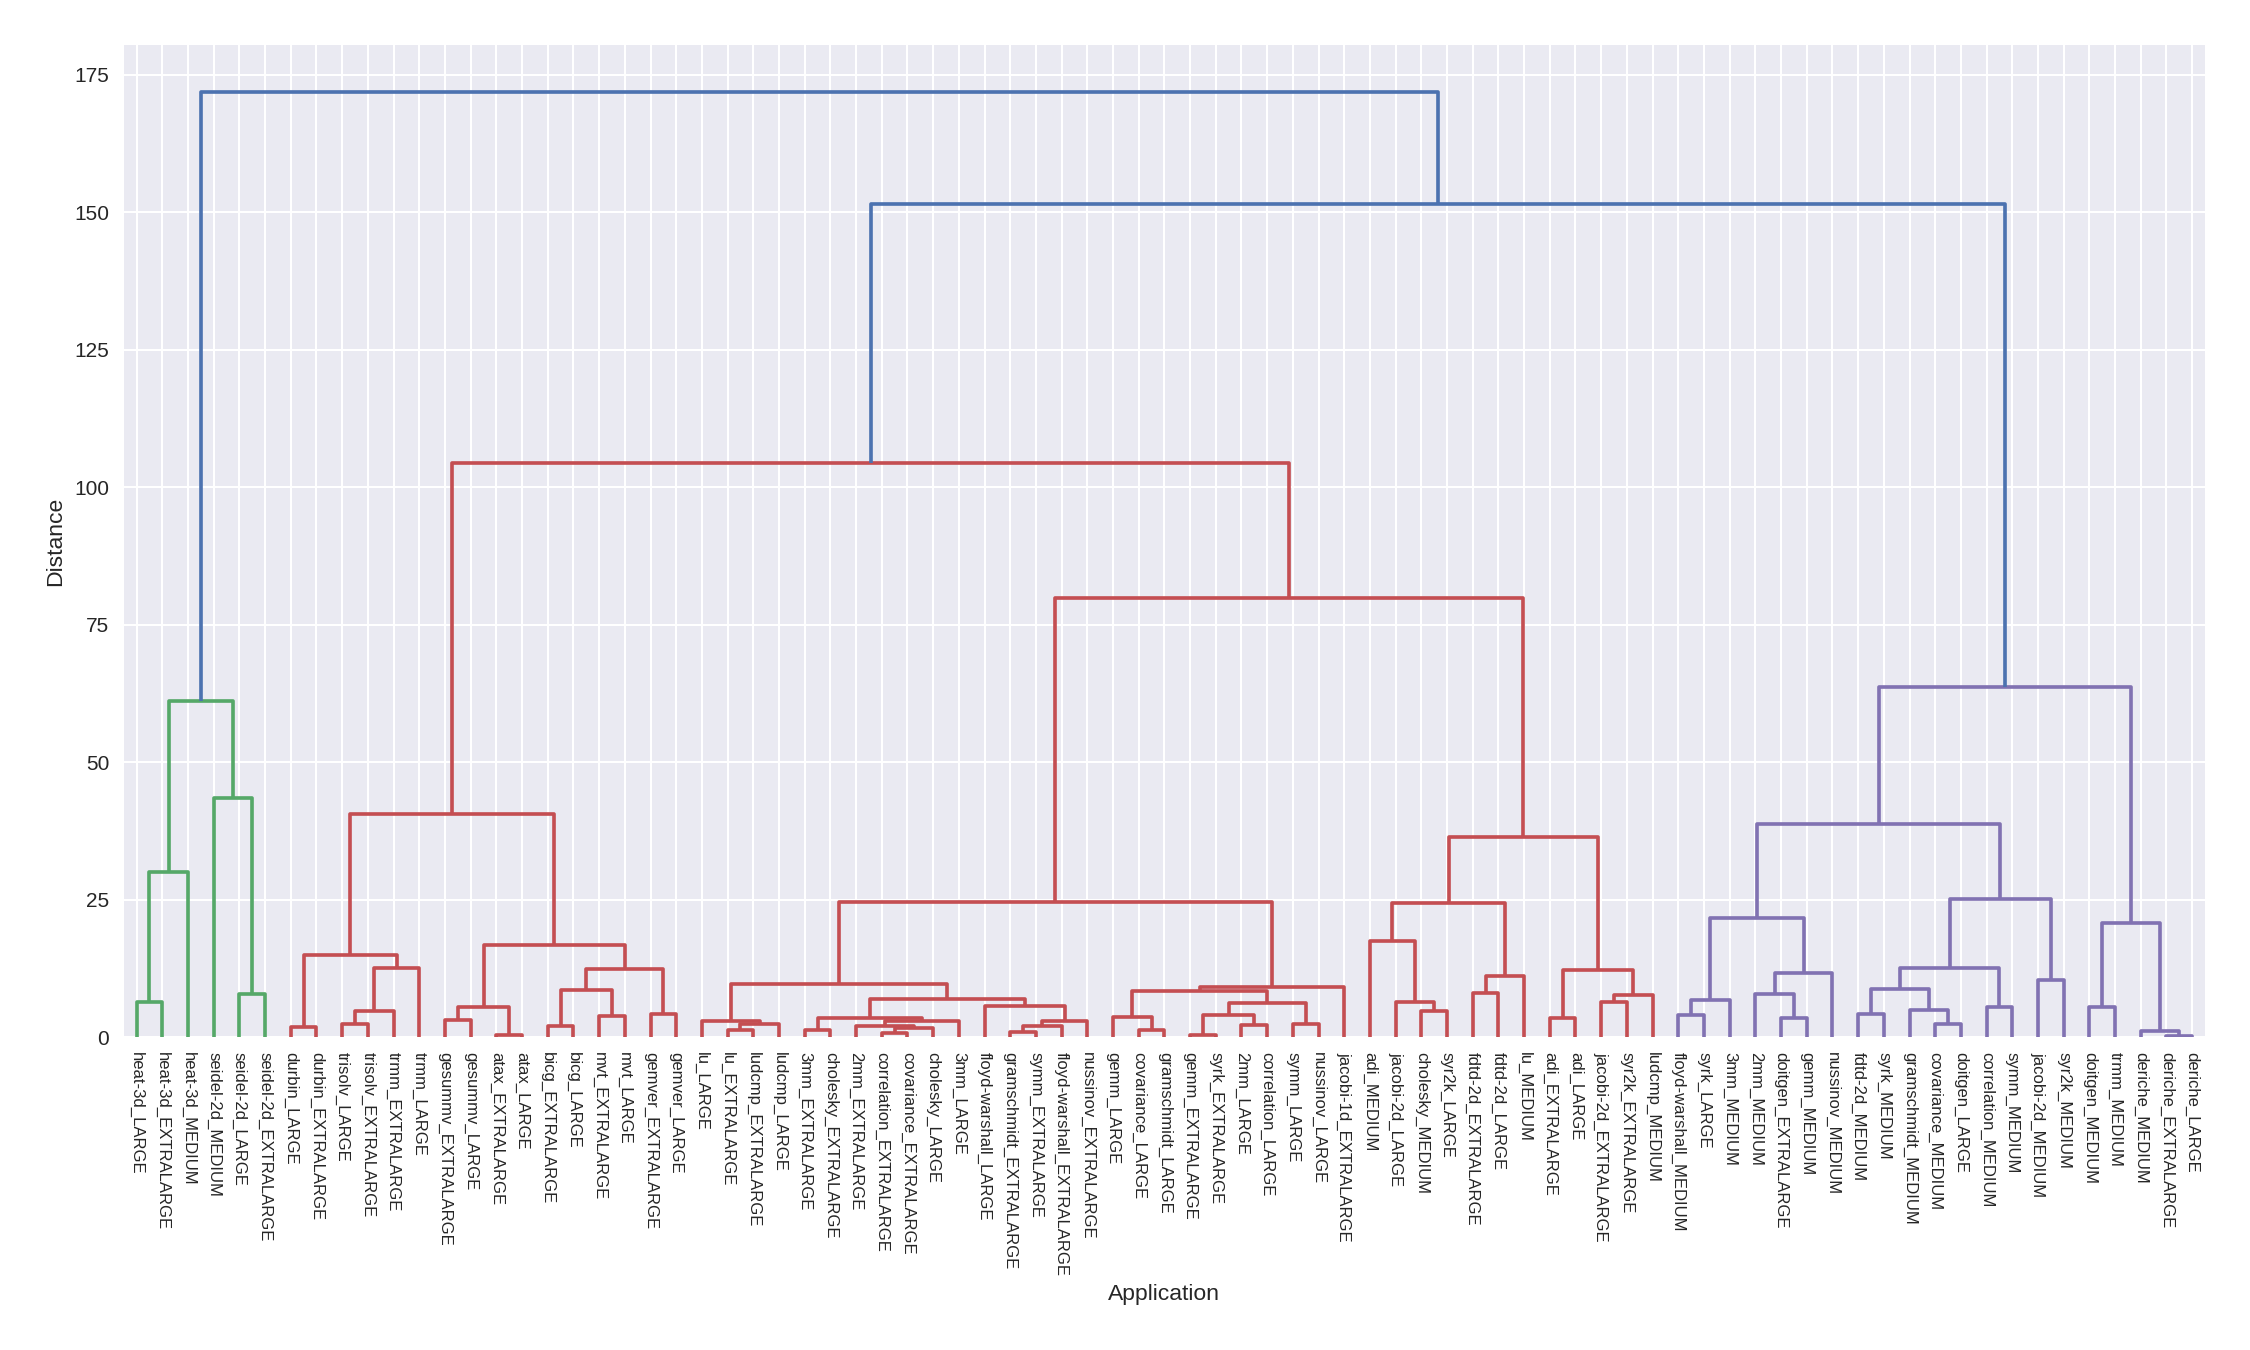
\includegraphics[width=\textwidth]{fingerprint/figures/dendograma_input_size.png}
%     \end{subfigure}
%     \\
%     \begin{subfigure}{\textwidth}
%         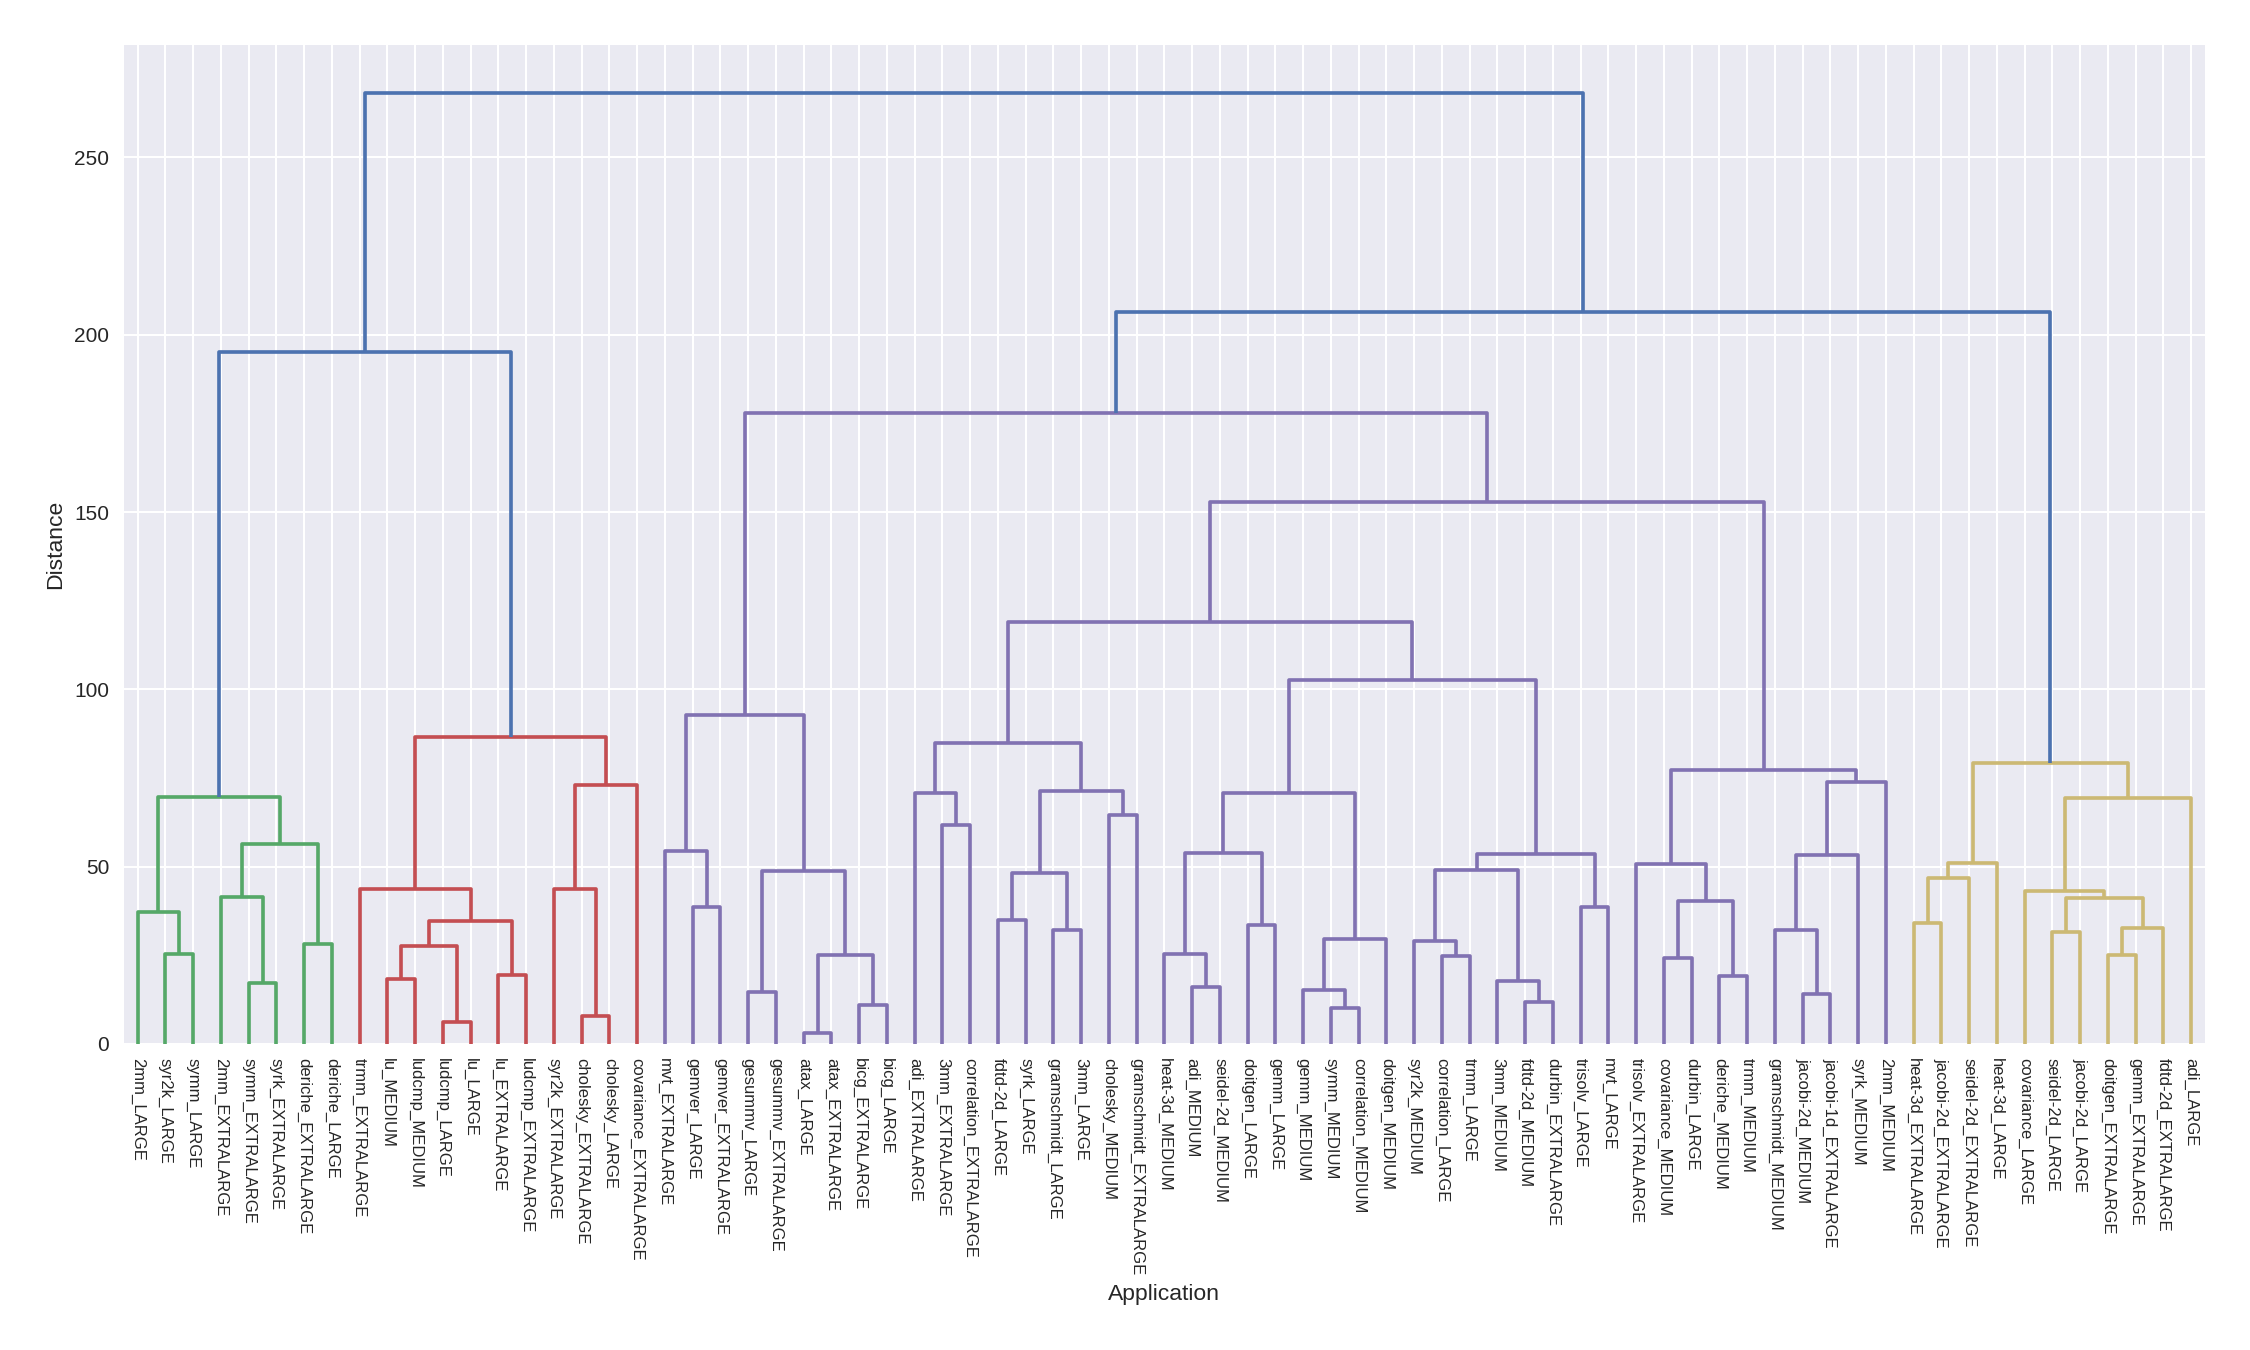
\includegraphics[width=\textwidth]{fingerprint/figures/dendograma_floating.png}
%     \end{subfigure}
%     %and so on
% \end{figure*}

To have an idea of how the behavior of the variable input size for each clusters is, it was plotted for the applications of clusters 1 and 2 shown on the figures \ref{fig:c1_input_size_0}, \ref{fig:c1_input_size_1}.

\begin{figure}[H]
	\centering
	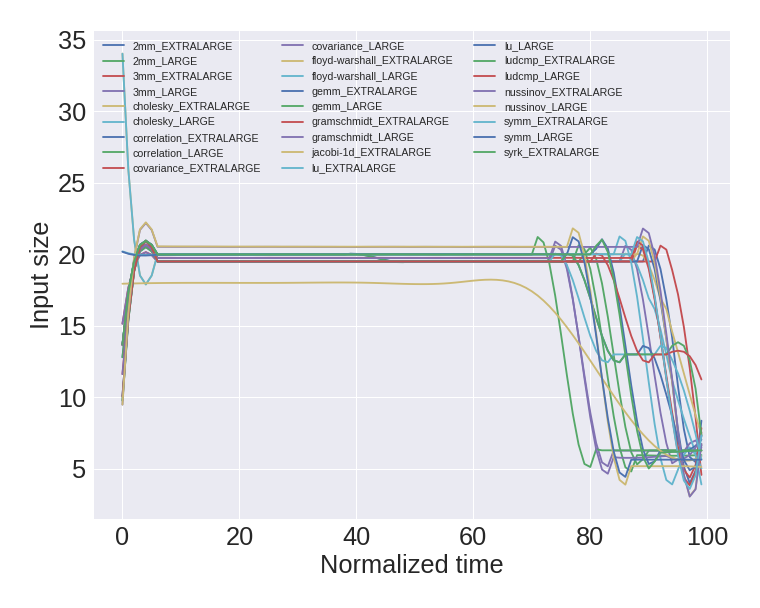
\includegraphics[width=\textwidth]{fingerprint/figures/cluster_input_0.png}
	\caption{Input size - Cluster 1}
	\label{fig:c1_input_size_0}
\end{figure}

From these figures, we can have an idea of what behavior was classified as the same class. On cluster 1 on the figure \ref{fig:c1_input_size_0} all applications showed the same behavior with approximately the same amplitude.

\begin{figure}[H]
	\centering
	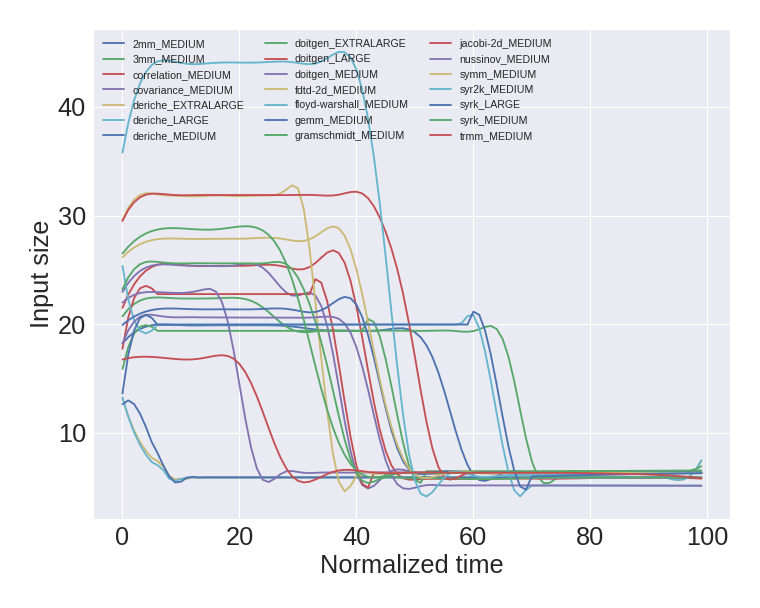
\includegraphics[width=\textwidth]{fingerprint/figures/cluster_input_1.png}
	\caption{Input size - Cluster 2}
	\label{fig:c1_input_size_1}
\end{figure}

On figure \ref{fig:c1_input_size_1} we observe that curves that have similar shape regardless of scale on vertical and horizontal axis have also been classified as the same clusters. This is the wanted comportment for the classification because we are only interested in the overall shape of the curve.


% \begin{figure}[H]
%     \centering
%     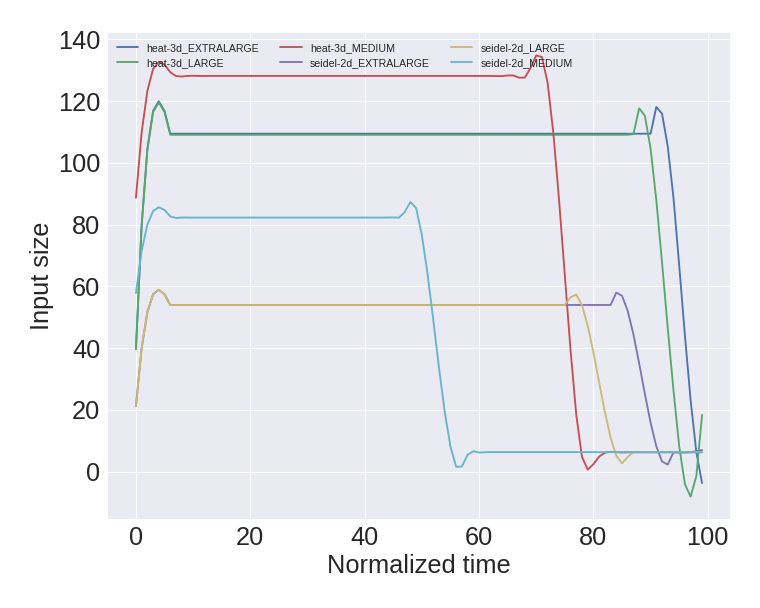
\includegraphics[width=\textwidth]{fingerprint/figures/cluster_input_4.png}
%     \caption{Input size - Cluster 3}
%     \label{fig:c1_input_size_2}
% \end{figure}

% To conclude this study we also clustering applications by its floating point behavior. For that we only use the counter correspondent to floating point operations. The figure \ref{fig:dendogram_fp} shows the dendrogram and the \ref{fig:sping_force_fp} the spring force graph plot.

% \begin{figure*}[h]
%     \includegraphics[width=\textwidth]{fingerprint/figuresdendograma_floating.png}
%     \caption{Dendrogram}
%     \label{fig:dendogram_fp}
% \end{figure*}

% \begin{figure}[H]
%     \centering
%     \includegraphics[width=\textwidth]{fingerprint/figures/graph_floating2.png}
%     \caption{Spring force of Canberra distance}
%     \label{fig:sping_force_fp}
% \end{figure}

% The figures \ref{fig:cluster_fp1},\ref{fig:cluster_fp2},\ref{fig:cluster_fp3} show the behavior on the same cluster for the float point operations. For this classification the number of clusters was 8.

% \begin{figure}[H]
%     \centering
%     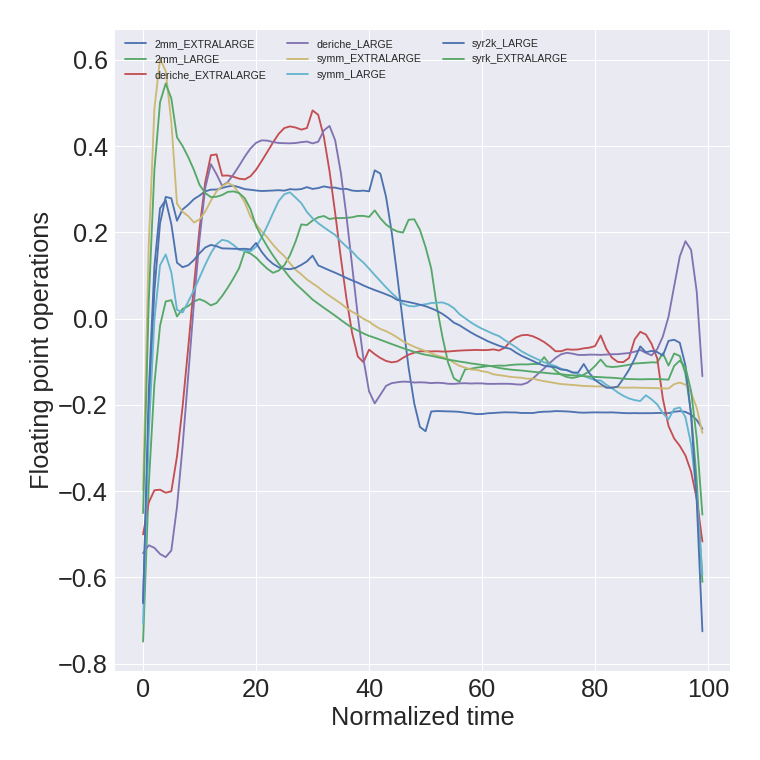
\includegraphics[width=\textwidth]{fingerprint/figures/cluster_fp_0.png}
%     \caption{Floating point - Cluster 1}
%     \label{fig:cluster_fp1}
% \end{figure}

% \begin{figure}[H]
%     \centering
%     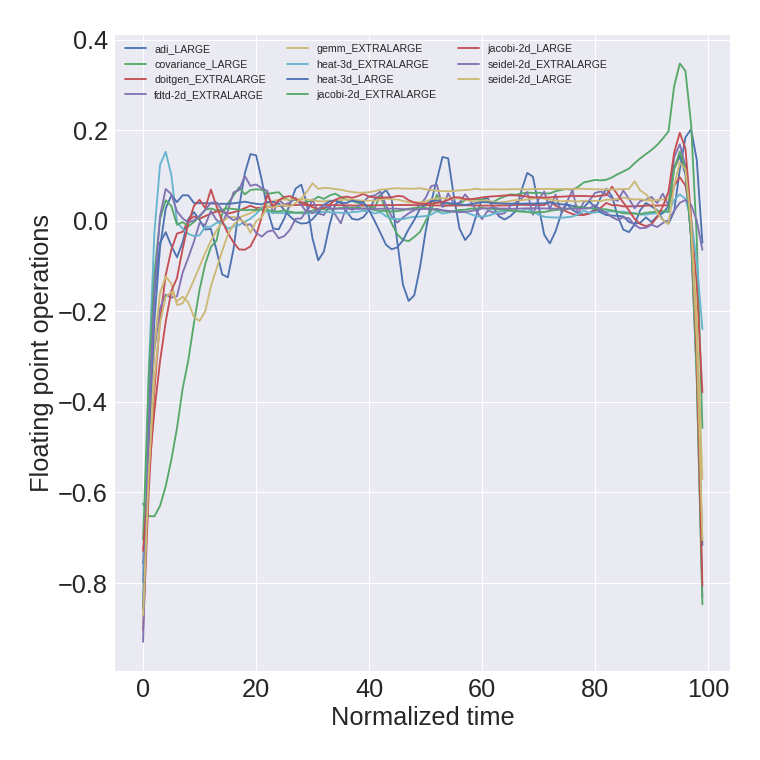
\includegraphics[width=\textwidth]{fingerprint/figures/cluster_fp_4.png}
%     \caption{Floating point - Cluster 2}
%     \label{fig:cluster_fp2}
% \end{figure}

% \begin{figure}[H]
%     \centering
%     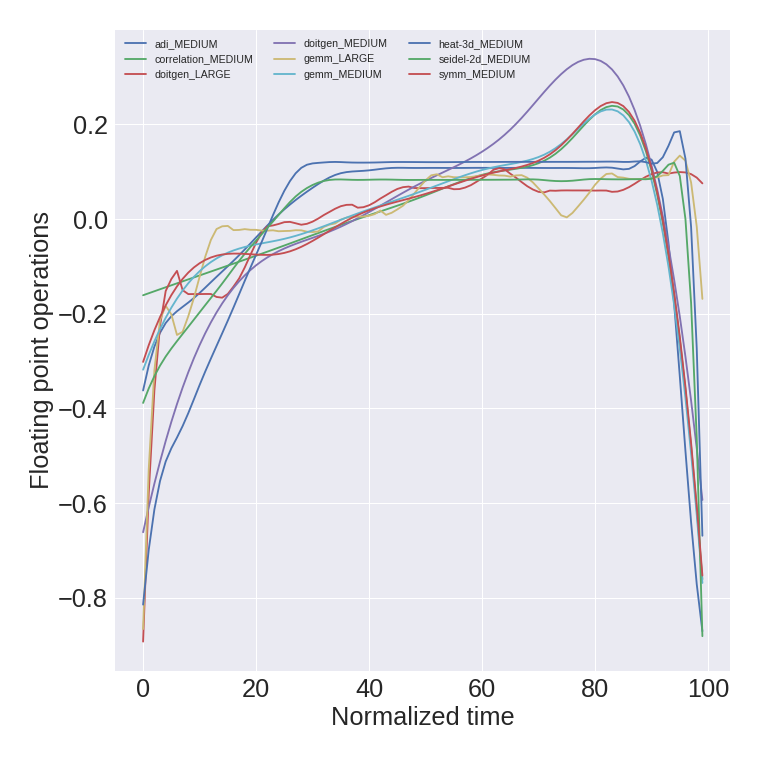
\includegraphics[width=\textwidth]{fingerprint/figures/cluster_fp_5.png}
%     \caption{Floating point - Cluster 3}
%     \label{fig:cluster_fp3}
% \end{figure}

% Here we can also observed again that applications with the same shape were classified as the same clusters.

\section{Validation the model} \label{sec:experimentalvalidation}
In this section, the models presented in~Sections \ref{sec:power_model} and~\ref{sec:performance_model} were validated with a benchmark specific for multi-core architectures. Additionally, in order to assess the modeling overhead and accuracy, our proposal was then compared to machine learning approaches. We compared against support vector regression (SVR)~\cite{Smola2004ARegression}, decision tree \cite{Kitts2006RegressionLecture}, k-nearest neighbors \cite{Altman1992AnRegression}, multilayer perceptron \cite{Murtagh1991MultilayerRegression}, and some new methods, such as Gao et al. \cite{Gao2019DendriticPrediction}. However, SVR was chosen as the most representative because it performed best in our tests without aggressive fine-tuning, as shown in \cref{fig:ml_models}.

\begin{figure}[H]
	\centering
	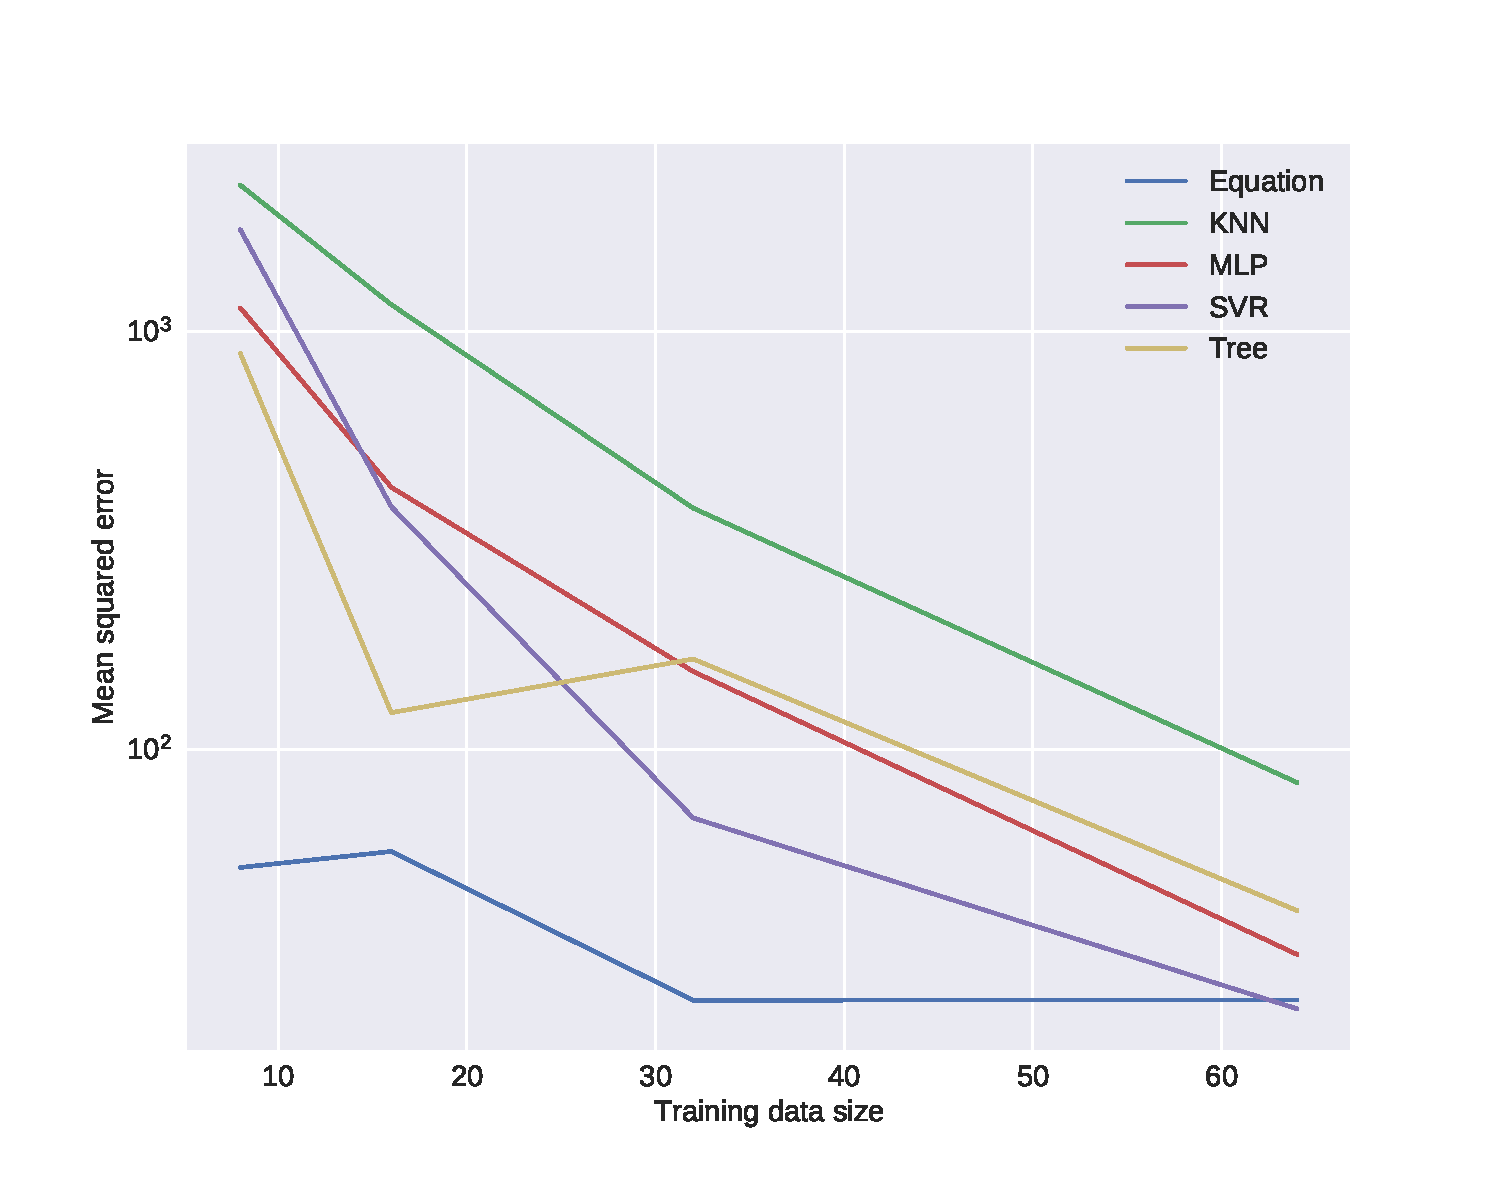
\includegraphics[width=\columnwidth]{experiments/figures/ml_models.pdf}
	\caption{Average of the mean squared error for all applications of our study case Section \ref{sec:casestudyapplication}.}
	\label{fig:ml_models}
\end{figure}

\subsection{Verifying Hypothesis}

In this section, we validate whether the assumptions of our model are valid for the system used.

\subsubsection{Frequency and Voltage Relation}
One of the assumptions was that the frequency and the voltage have a linear relationship, as indicated by ~\cref{eq:f_v}. To verify that, we build an experiment that sets the frequency to a specific value while sampling the voltage using the APERF and MPERF registers that provide feedback on the current CPU frequency. The average result of the sampling voltages is shown in  \cref{fig:freq_volt_rel}, where we can observe a near-perfect linear relation. This is because manufacturers implement this curve in the processors, using tables that relate ranges of frequencies to voltages so that they can precisely define any curve that will better suit their design.

\begin{figure}[H]
	\centering
	\captionsetup[subfigure]{justification=centering}
	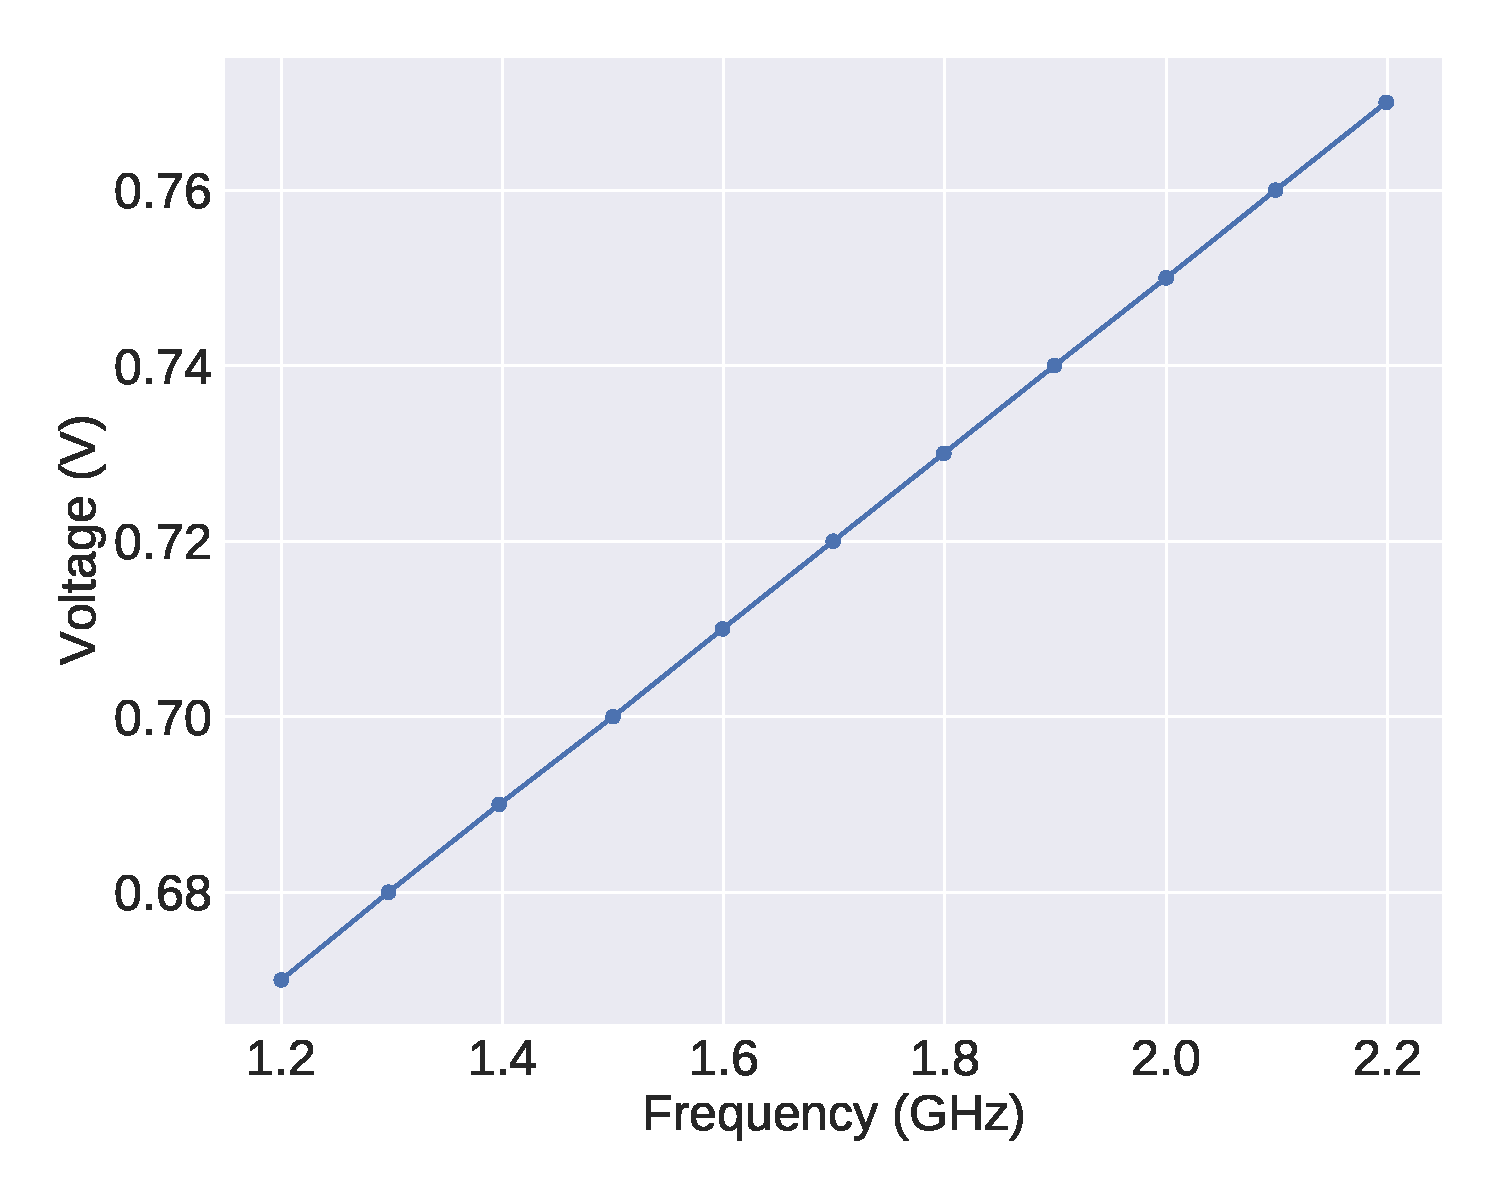
\includegraphics[width=\columnwidth]{experiments/figures/freq_volt_rel.pdf}
	\caption{Frequency voltage relation.}
	\label{fig:freq_volt_rel}
\end{figure}

\subsubsection{Input Size and Instructions}
We ran the applications with different inputs assuming  linear growth in the amount of work for one input to the other when building our model. However, measuring and controlling the amount of work would require much instrumentation and tuning to find an input corresponding to a certain amount of work. Therefore, to build our models, we use the time to reference the amount of work, assuming that the work is proportional to the executing time. \cref{fig:time_input} corresponds to the verification of this supposition.


\cref{tab:corr_in_time} shows that the assumption was reasonable since the average correlation was 0.96 for all applications, indicating that growth in the number of instructions  will follow the time. This was the case for all applications that we ran in our benchmark and should hold for any data parallelism type of application.
\begin{figure}[H]
	\centering
	\captionsetup[subfigure]{justification=centering}
	\begin{subfigure}[b]{0.45\textwidth}
		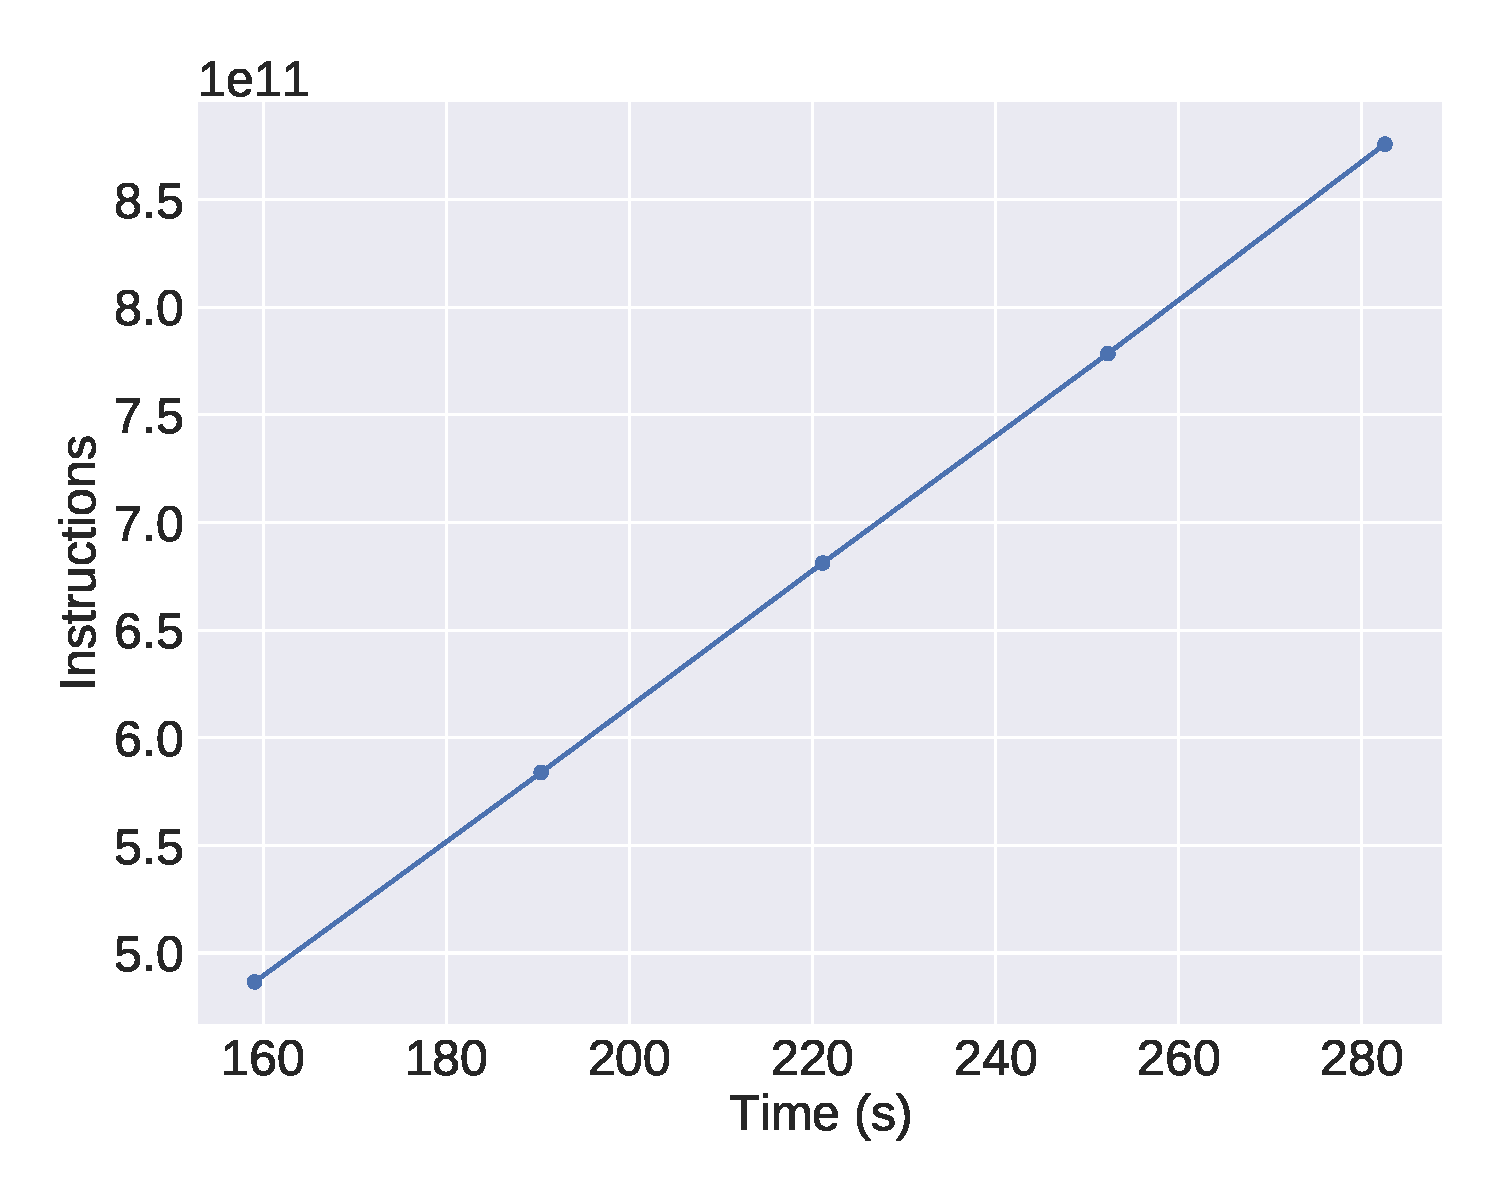
\includegraphics[width=\columnwidth]{models/figures/hypothesis/input_instructions/input_time/blackscholes.pdf}
		\caption{Blackscholes.}
		\label{fig:time_input_blackshoels}
	\end{subfigure}
	%
	\begin{subfigure}[b]{0.45\textwidth}
		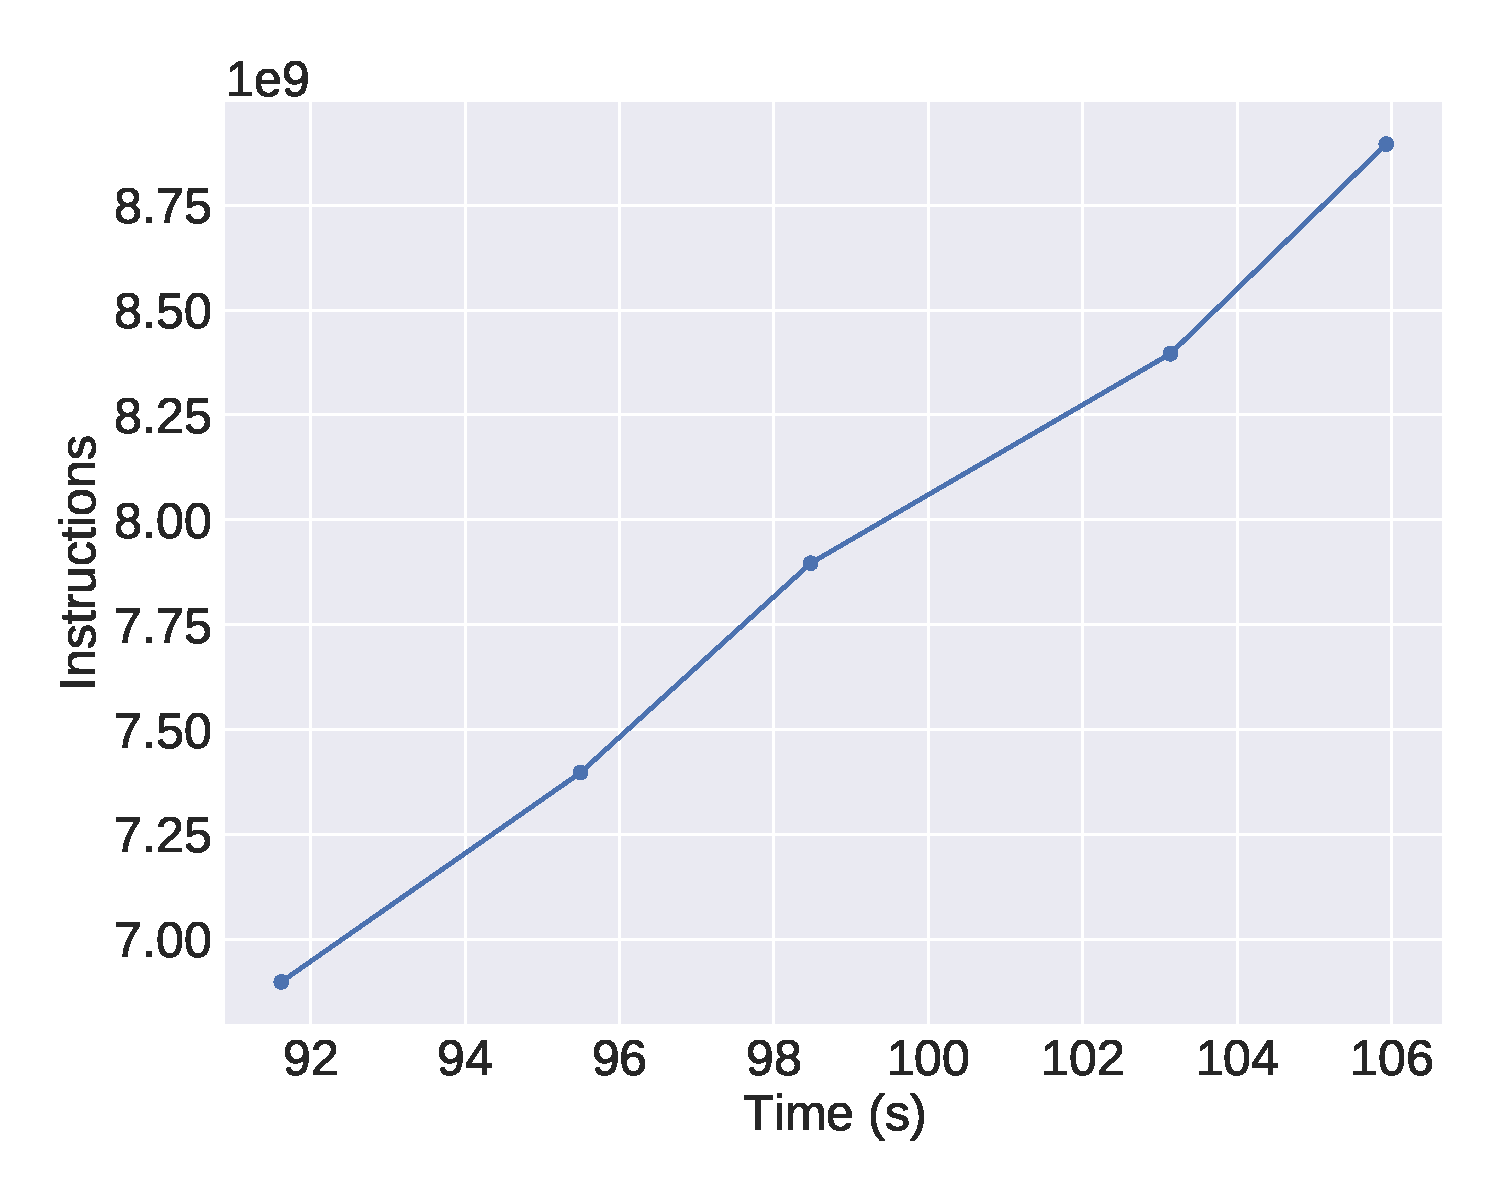
\includegraphics[width=\columnwidth]{models/figures/hypothesis/input_instructions/input_time/canneal.pdf}
		\caption{Canneal.}
		\label{fig:time_input_canneal}
	\end{subfigure}
	
	\hfill
	\caption{Relation between time and instructions for each input size. }
	\label{fig:time_input}
\end{figure}
\vspace{-6pt}

\begin{table}[H]
	\centering
	\caption{Correlation of time and instructions for all applications.}
	\begin{tabular}{ll}
		\multicolumn{1}{l|}{\textbf{Application}} & \textbf{Correlation} \\ \hline
		Blackscholes                                               & 0.99                                  \\
		Bodytrack                                                  & 0.99                                  \\
		Canneal                                                    & 0.99                                  \\
		Dedup                                                      & 0.99                                  \\
		Ferret                                                     & 0.96                                  \\
		Fluidanimate                                               & 0.99                                  \\
		Freqmineq                                                  & 0.99                                  \\
		Openmc                                                     & 0.94                                  \\
		Raytrace                                                   & 0.99                                  \\
		Swaptions                                                  & 0.99                                  \\
		Vips                                                       & 0.98                                  \\
		x264                                                       & 0.99                                  \\
		HPL                                                        & 0.79                                  \\ \hline
	\end{tabular}
	\label{tab:corr_in_time}
\end{table}

The next assumption was that the application's behavior was the same when varying the workload. This condition is necessary for using the model with an unknown input size because, if the behavior is the same, we can interpolate the known inputs. One way to verify this is to measure the rate of instructions per second normalized by the frequency, as shown in \cref{fig:fingerpritns}.
\begin{figure}[H]
	\centering
	\captionsetup[subfigure]{justification=centering}
	
	\begin{subfigure}[b]{0.45\textwidth}
		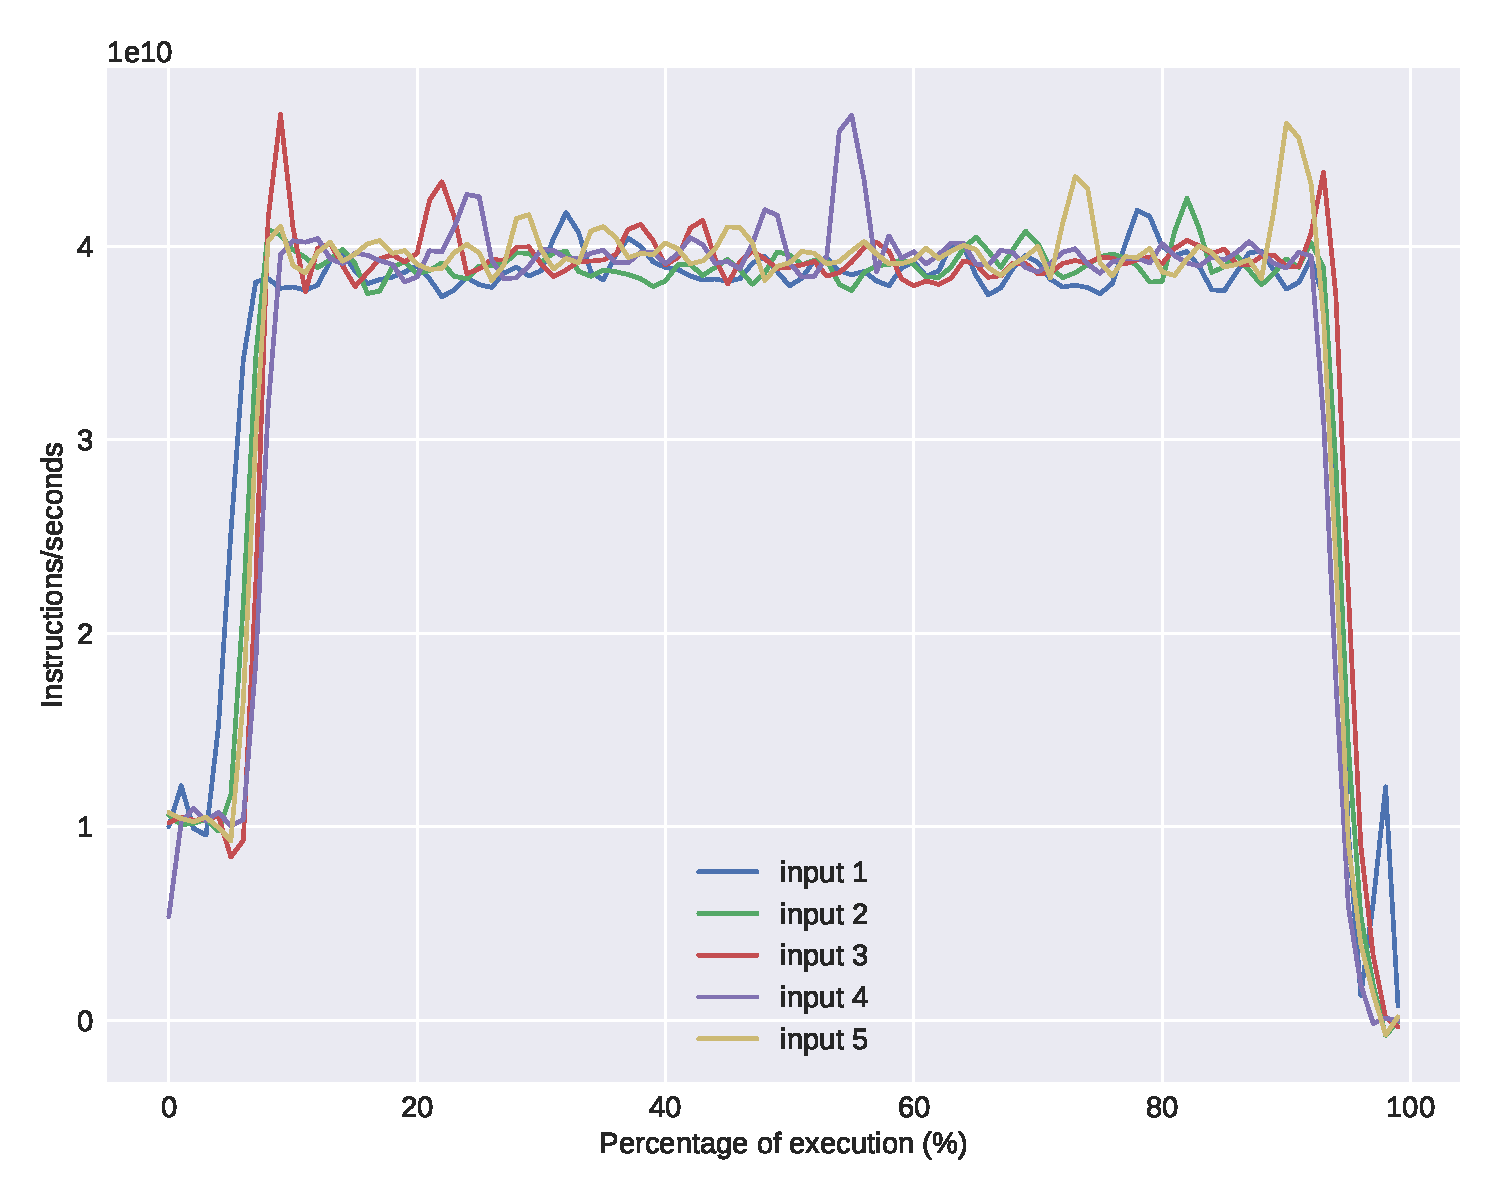
\includegraphics[width=\columnwidth]{models/figures/hypothesis/input_instructions/fp/blackscholes.pdf}
		\caption{Blacksholes.}
		\label{fig:fp_baclscholes}
	\end{subfigure}
	%
	\begin{subfigure}[b]{0.45\textwidth}
		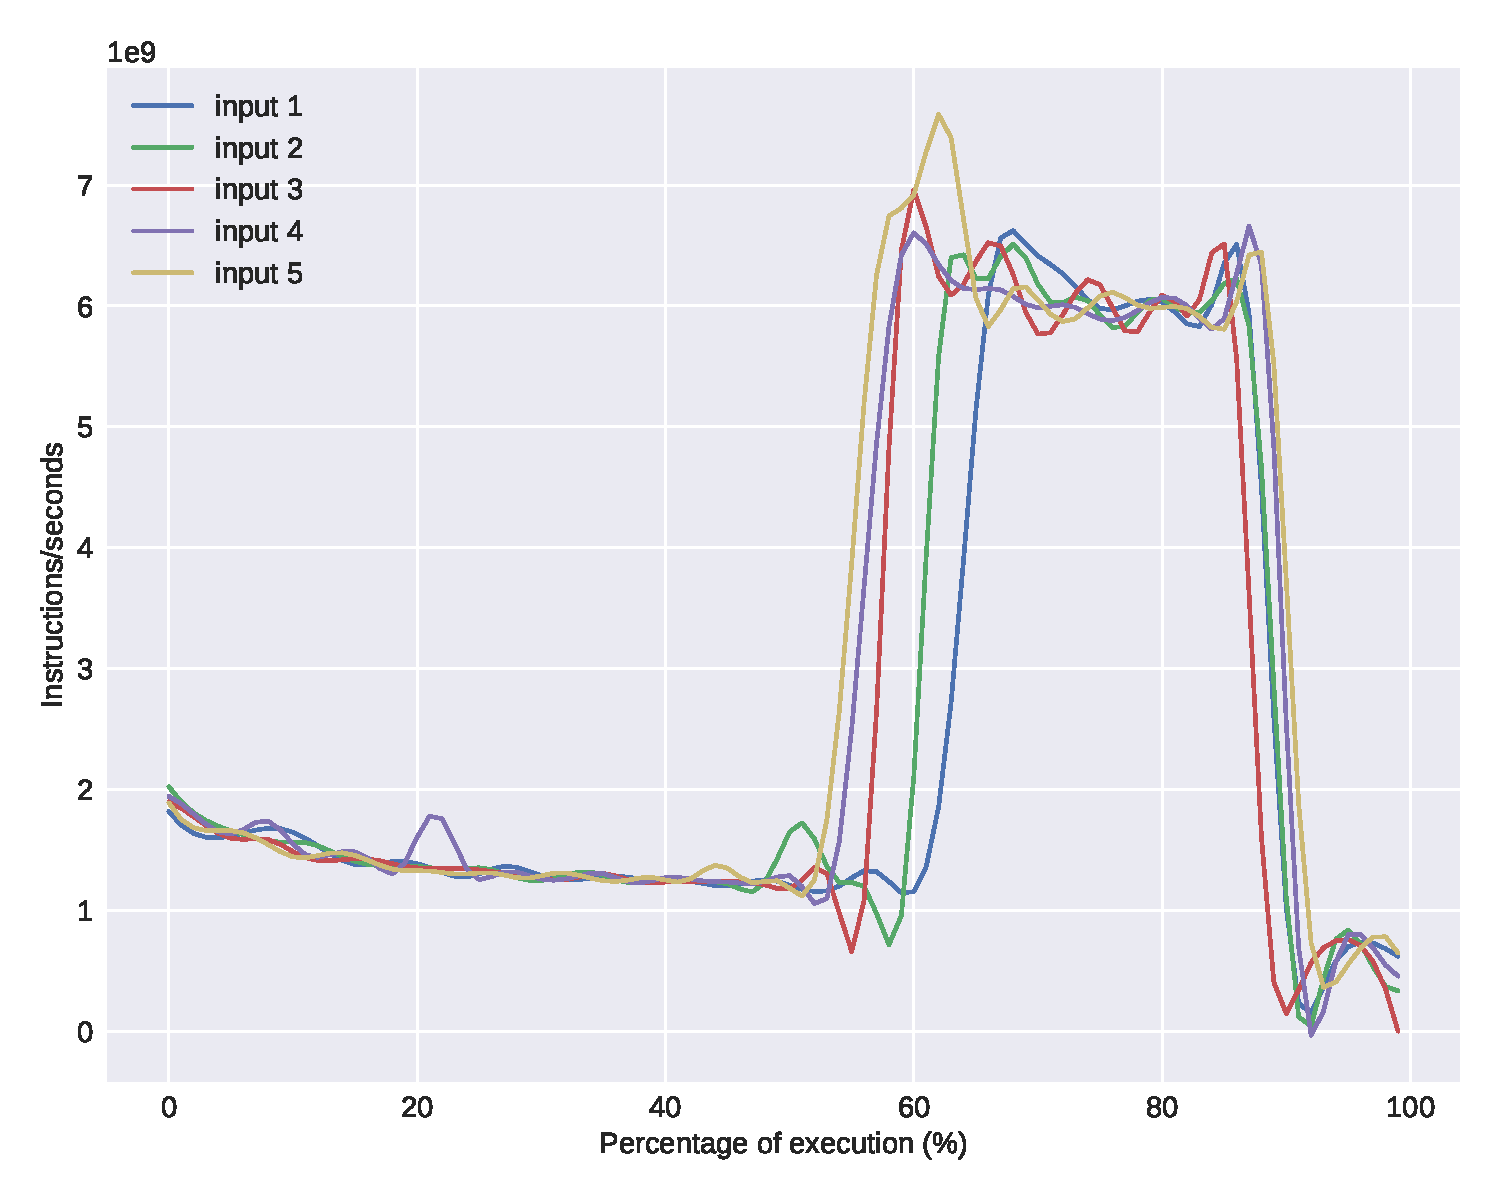
\includegraphics[width=\columnwidth]{models/figures/hypothesis/input_instructions/fp/canneal.pdf}
		\caption{Canneal.}
		\label{fig:fp_canneal}
	\end{subfigure}
	
	\hfill
	\caption{Rate of instructions per second varying the input size normalized by the frequency.}
	\label{fig:fingerpritns}
\end{figure}

\cref{fig:fingerpritns} shows that the applications have roughly the same curve when normalized; this also happens for all other applications in our benchmark.

The final assumption is that the workload should also not vary depending on the number of cores or frequency. To verify, we measure the total number of executed instructions while varying the cores from 1 to 32. \cref{tab:cores_variation} shows the results.

\begin{table}[H]
	\centering
	\caption{Variation of the number of instructions when changing the number of cores for the same input.}
	%\begin{tabular}{c|c|c|c}
	\begin{tabular*}{\hsize}{@{\extracolsep{\fill}}cccc}
		\toprule
		& \textbf{Average} & \textbf{Standard}     & \textbf{Standard}\\
		\multirow{-2}{*}{\textbf{Application}}& \textbf{Number of Instructions} & \textbf{Deviation}     & \textbf{Deviation} \textbf{(\%) }\\ \midrule
		Vip          & $7.97 \times 10^{11}$     & $7.16 \times 10^{6}$  & 0.00 \\ %Please use Scientific notation. For example, “1.65e+04” should be changed to “1.65× 104”. Please confirm `%` whether to remove.
		Openmc       & $8.17 \times 10^{7}$     & $ 1.65 \times 10^{4}$ & 0.02    \\ 
		Rtview       & $9.91 \times 10^{12}$     & $ 1.55 \times 10^{9}$ & 0.02    \\ 
		X264         & $4.52 \times 10^{11}$     & $ 5.81 \times 10^{7}$ & 0.01    \\ 
		Bodytrack    & $1.86 \times 10^{12}$     & $ 3.95 \times 10^{10}$ & 2.13    \\ 
		Fluidanimate & $2.09 \times 10^{12}$     & $ 8.44 \times 10^{10}$ & 4.04    \\ 
		HPL          & $1.14 \times 10^{8}$      & $ 1.24 \times 10^{5}$ & 0.11    \\ 
		Blackschole  & $3.75 \times 10^{12}$     & $ 1.40 \times 10^{9}$ & 0.04     \\ 
		Dedup        & $1.02 \times 10^{11}$     & $ 5.74 \times 10^{7}$ & 0.06     \\ 
		Swapti       & $2.43 \times 10^{12}$     & $ 8.87 \times 10^{8}$ & 0.04     \\ 
		Canneal      & $1.19 \times 10^{11}$     & $ 4.46 \times 10^{7}$ & 0.04     \\ 
		Freqmine     & $1.27 \times 10^{12}$     & $ 4.78 \times 10^{8}$ & 0.04     \\ 
		Ferret       & $4.76 \times 10^{11}$     & $ 7.04 \times 10^{7}$ & 0.01     \\ \bottomrule
	\end{tabular*}
	\label{tab:cores_variation}
\end{table}
% Corrected

\cref{tab:cores_variation} shows the standard deviation and what that corresponds to in terms of the total number of instructions as a percentage. 

The same test was performed for the frequency, varying from 1.2 to 2.2 GHz with 100~MHz steps. The results are shown in \cref{tab:freq_variation}.

These results show that all the assumptions were reasonable, and we can safely move to the validation of the model's prediction.
\begin{table}[H]
	\caption{Variation of the number of instructions when changing the frequency for the same input.}
	\centering
	%\begin{tabular}{c|c|c|c}{\hsize}{@{\extracolsep{\fill}}cccc}
	\begin{tabular*}{\hsize}{@{\extracolsep{\fill}}cccc}
		\toprule
		& \textbf{Average} & \textbf{Standard}     & \textbf{Standard}\\
		\multirow{-2}{*}{\textbf{Application}}& \textbf{Number of Instructions} & \textbf{Deviation}     & \textbf{Deviation} \textbf{(\%)} \\ \midrule
		Vip          & $7.97 \times 10^{11}$      & $ 1.16 \times 10^{6}$  & 0.00      \\ 
		Openmc       & $8.17 \times 10^{7}$       & $ 4.52 \times 10^{3}$  & 0.01      \\ 
		Rtview       & $9.91 \times 10^{12}$      & $ 6.64 \times 10^{5}$  & 0.00      \\ 
		X264         & $4.52 \times 10^{11}$      & $ 1.54 \times 10^{5}$  & 0.00      \\ 
		Bodytrack    & $1.84 \times 10^{12}$      & $ 2.54 \times 10^{5}$  & 0.00      \\ 
		Fluidanimate & $2.38 \times 10^{12}$      & $ 1.70 \times 10^{9}$  & 0.07      \\ 
		HPL          & $1.14 \times 10^{8}$       & $ 5.95 \times 10^{3}$  & 0.01      \\ 
		Blackschole  & $3.75 \times 10^{12}$      & $ 4.36 \times 10^{5}$  & 0.00      \\ 
		Dedup        & $1.02 \times 10^{11}$      & $ 8.32 \times 10^{7}$  & 0.08      \\ 
		Swapti       & $2.43 \times 10^{12}$      & $ 1.48 \times 10^{5}$  & 0.00      \\ 
		Canneal      & $1.19 \times 10^{11}$      & $ 3.01 \times 10^{5}$  & 0.00      \\ 
		Freqmine     & $1.27 \times 10^{12}$      & $ 3.70 \times 10^{8}$  & 0.03      \\ 
		Ferret       & $4.76 \times 10^{11}$      & $ 5.63 \times 10^{7}$  & 0.01      \\\bottomrule
	\end{tabular*}
	\label{tab:freq_variation}
\end{table}


\subsection{Fitting the Models} \label{subsec:fitting}
To find the parameters of  \cref{eq:en_final}, 10 uniformly random configurations of frequencies ($f$), cores ($p$) and inputs ($N$) were chosen from the range $1<=p<=32$, $1.2<=f<=2.2$ and $1<=N<=5$, respectively. The application was executed for each chosen configuration, and the measured energy and time values were collected. For the input size, if we assume that all CPU instructions take approximately the same time to execute, the number of basic operations will be directly correlated with the time. Thus, we can estimate the input size by looking at the execution time, allowing us to divide a large input size into several smaller ones, knowing their relationship, as performed in the work of Oliveira ~\cite{Oliveira2018ApplicationCharacterization}. The unity can also vary depending on the definition. For simplicity, we assign numbers from 1 to 10, increasing the problem linearly, so it is also possible to interpolate any input in between these values.

For each configuration, samples of the power were collected using IPMI every 1 second. This sampling rate was chosen based on the magnitude of the mean run time of the applications, which is in the order of minutes. Therefore, this rate provides enough samples to measure average power. Additionally, timestamps and the total run time were collected. The total energy spent on each configuration is estimated by first interpolating the power samples using the first-order method and then integrating this function in the time.

The model's parameters are calculated by solving an optimization problem of finding the values that minimize the squared error of the prediction to the measured values using the non-linear least-squares method.

The Python library Scikit-Learn was used to build the SVR model~\cite{Pedregosa2011Scikit-learn:Python}. The SVR was trained using the same data used for parameter estimation of Equation (\ref{eq:en_final}) %\cref{eq:en_final}
with a grid search used to find the best kernel function and the best values for the hyper-parameters penalty for the wrong ($C$) and ($\gamma$). For this data, the best function was the radial base function (RBF), and the hyper-parameters were $C=10^4$ and $\gamma=0.5$.


\subsection{Measured versus Modeled Energy}
\label{subsec:measuredversusmodeledenergy}

To validate the model, we ran all possible configurations in the tested machine, varying the cores in a range of $1<=p<=32$, the frequency in $1.2<=f<=2.2$, and the input in $1<=N<=5$. The total number of configurations varies from 400 to over 1000 depending on the application, as some applications have restrictions on the number of cores that they can run. Once the data was collected, we computed the mean percentage error (MPE) according to the following equation:
\begin{equation}
	MPE = \frac{1}{N} \sum_i^N \frac{|y_{\rm estimated}-y_{\rm measured}|}{y_{\rm measured}}.
	\label{eq:mpe}
\end{equation}

\subsubsection{Frequency $\times$ Cores}
\cref{fig:en_eq_freq_cores_fc} plots the measured and modeled energy consumption for some of the applications modeled. In addition,  some of the possible shapes that the model can take while varying the number of active cores, and operating frequency, are shown.%please confirm that the intended meaning has been retained.
% yes its the same

\begin{figure}[H]
	\centering
	\captionsetup[subfigure]{justification=centering}
	\begin{subfigure}[b]{0.45\textwidth}
		\centerline{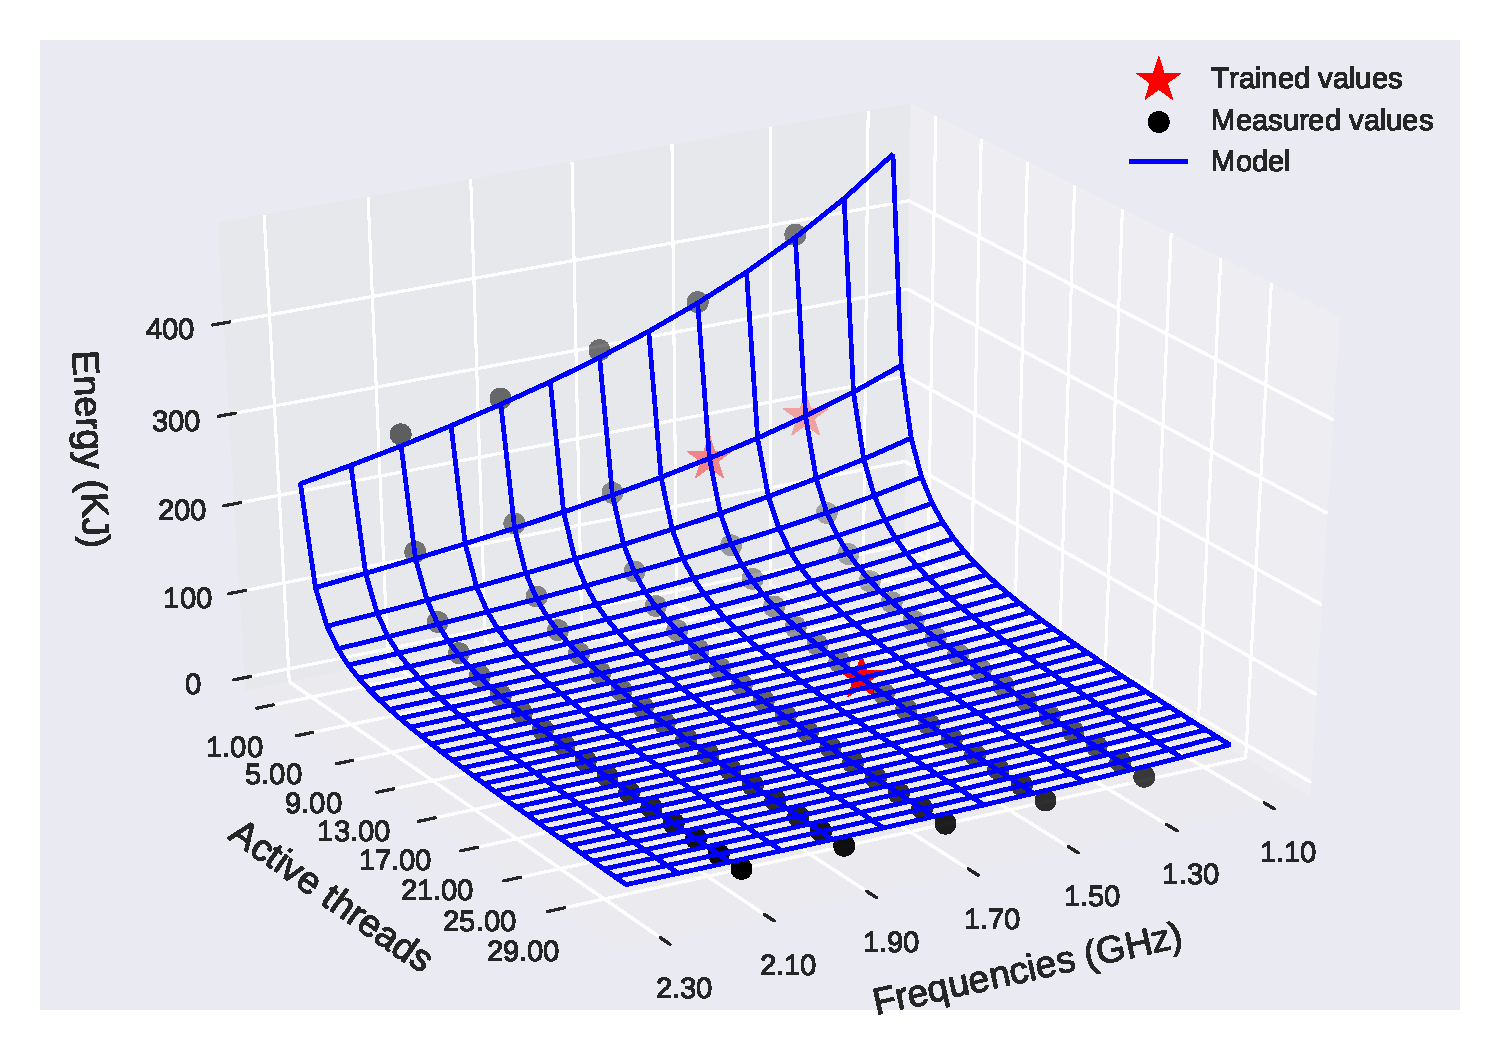
\includegraphics[width=\columnwidth]{models/figures/energy/freq_cores/completo_black_5.pdf}}
		\caption{}
		\label{fig:en_eq_black_fc}
	\end{subfigure}
	%
	\begin{subfigure}[b]{0.45\textwidth}
		\centerline{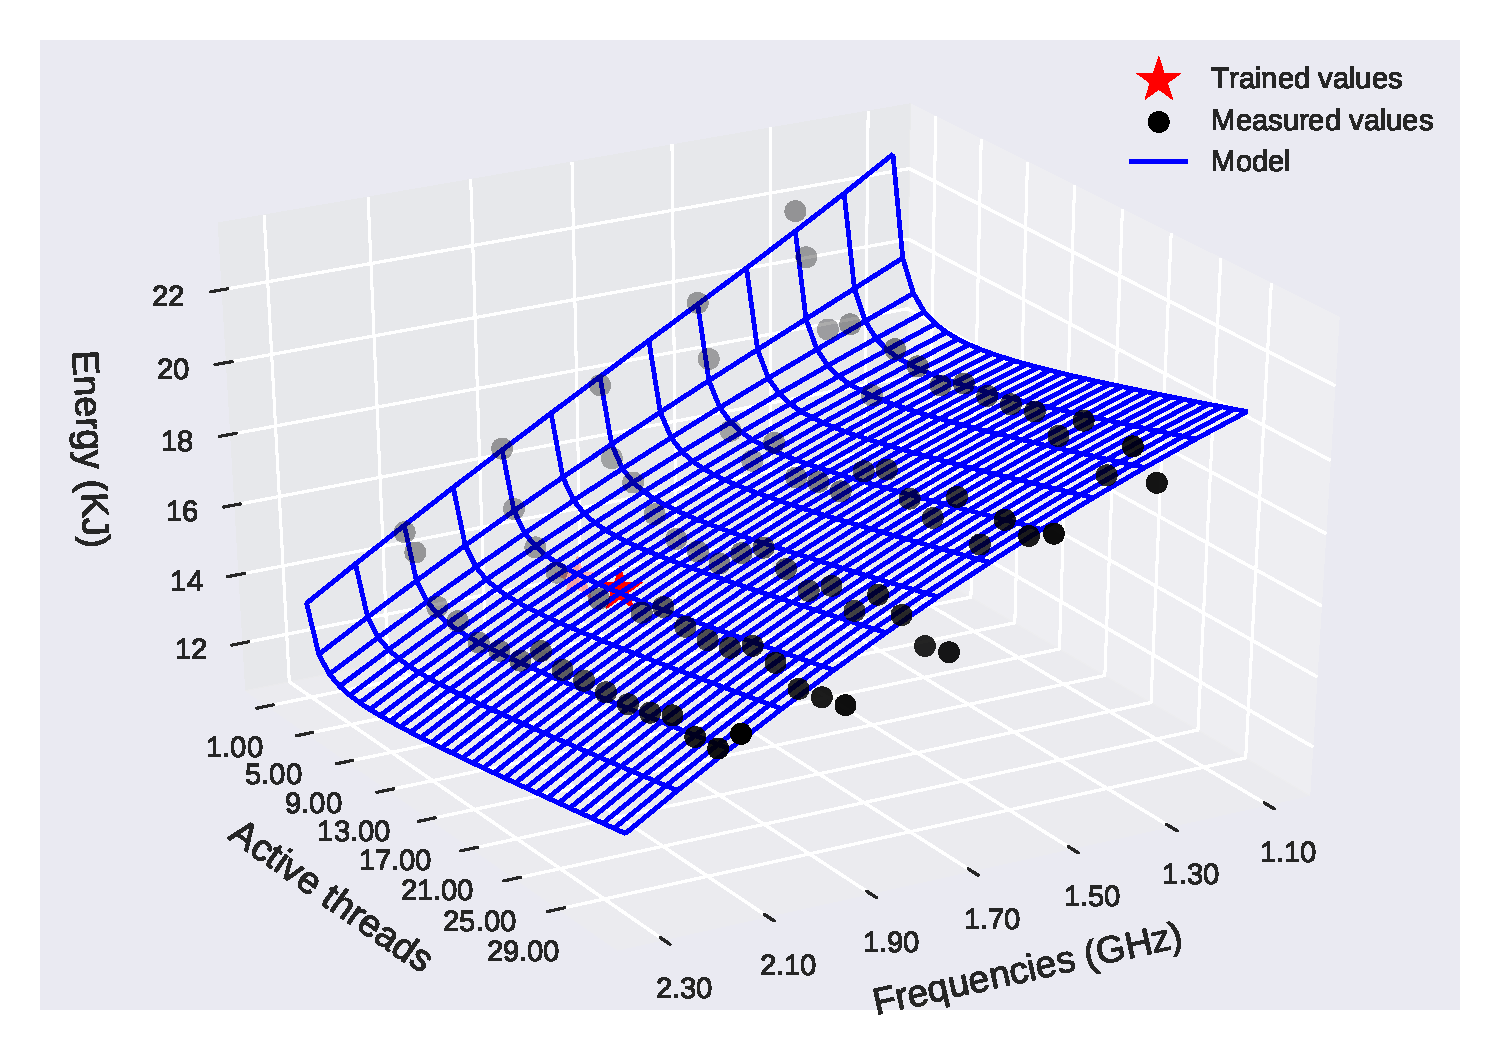
\includegraphics[width=\columnwidth]{models/figures/energy/freq_cores/completo_canneal_1.pdf}}
		\caption{}
		\label{fig:en_eq_canneal_fc}
	\end{subfigure}
	
	\caption{Example fit for a specific input size: Blackscholes (\textbf{a}) and Canneal (\textbf{b}).  “measured values” are the sensor data, and “minimum energy” is the minimum energy model prediction.
	}
	\label{fig:en_eq_freq_cores_fc}
\end{figure}
\subsubsection{Frequency $\times$ Input}
\cref{fig:en_eq_freq_inp_fi} plots the measured and modeled energy consumption for some of the applications modeled. The diagrams show some of the possible shapes that the model can take while varying the operating frequency, and input size.
\begin{figure}[H]
	\centering
	\captionsetup[subfigure]{justification=centering}
	\begin{subfigure}[b]{0.45\textwidth}
		\centerline{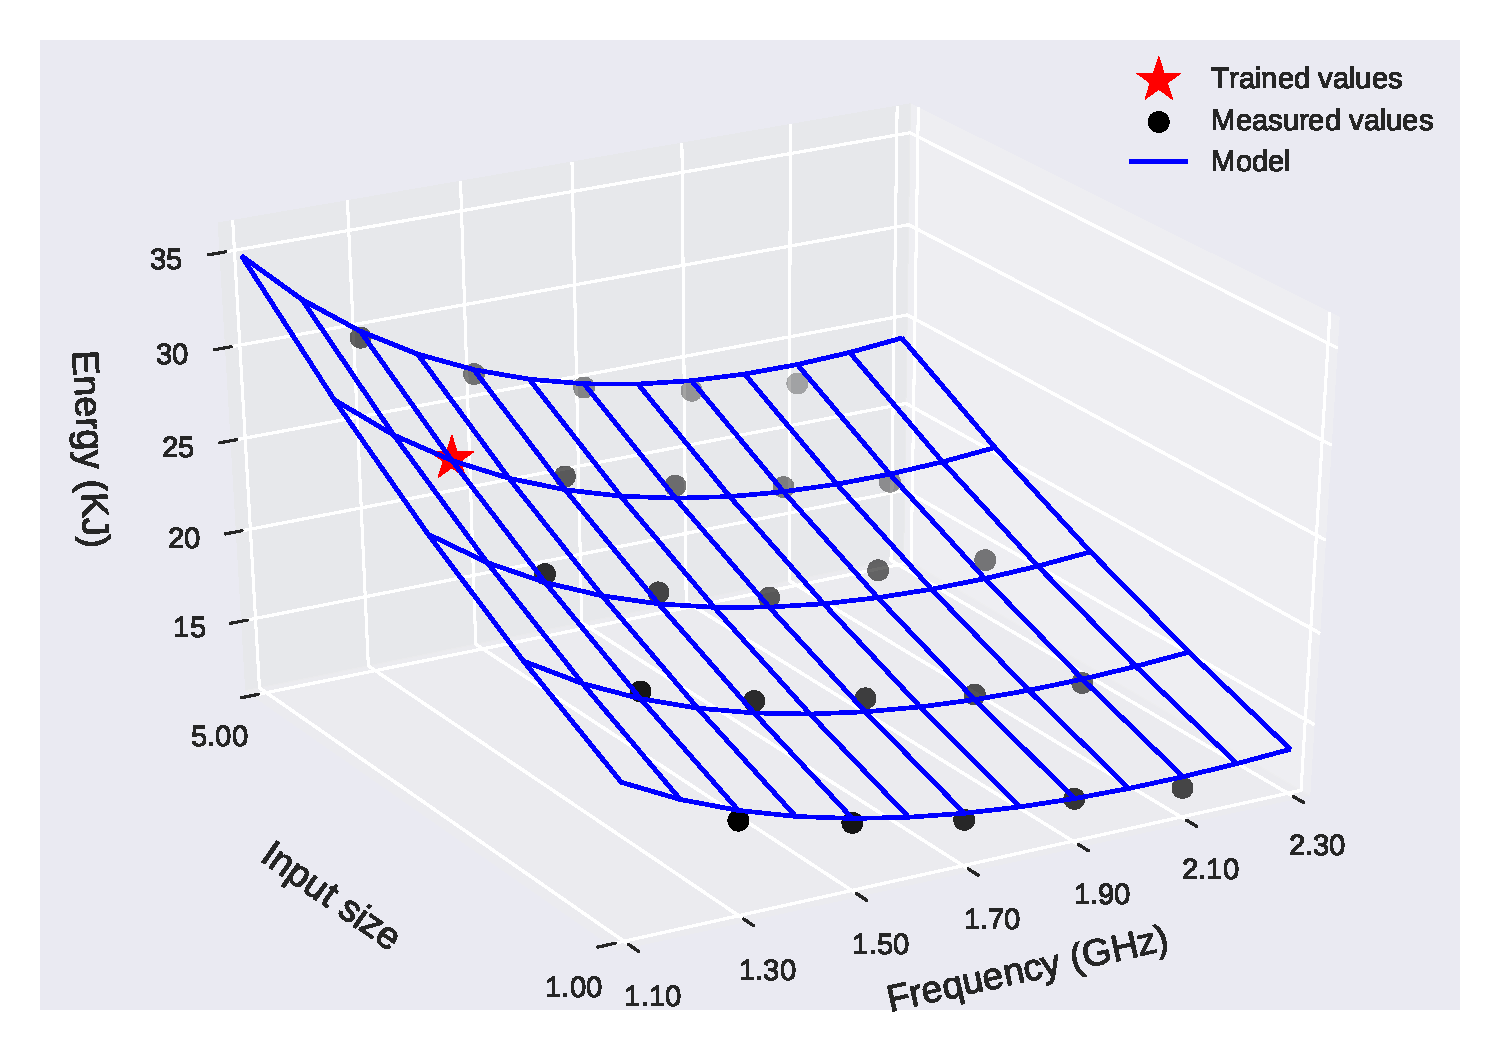
\includegraphics[width=\columnwidth]{models/figures/energy/freq_inps/completo_black_5.pdf}}
		\caption{}
		\label{fig:en_eq_black_fi}
	\end{subfigure}
	%
	\begin{subfigure}[b]{0.45\textwidth}
		\centerline{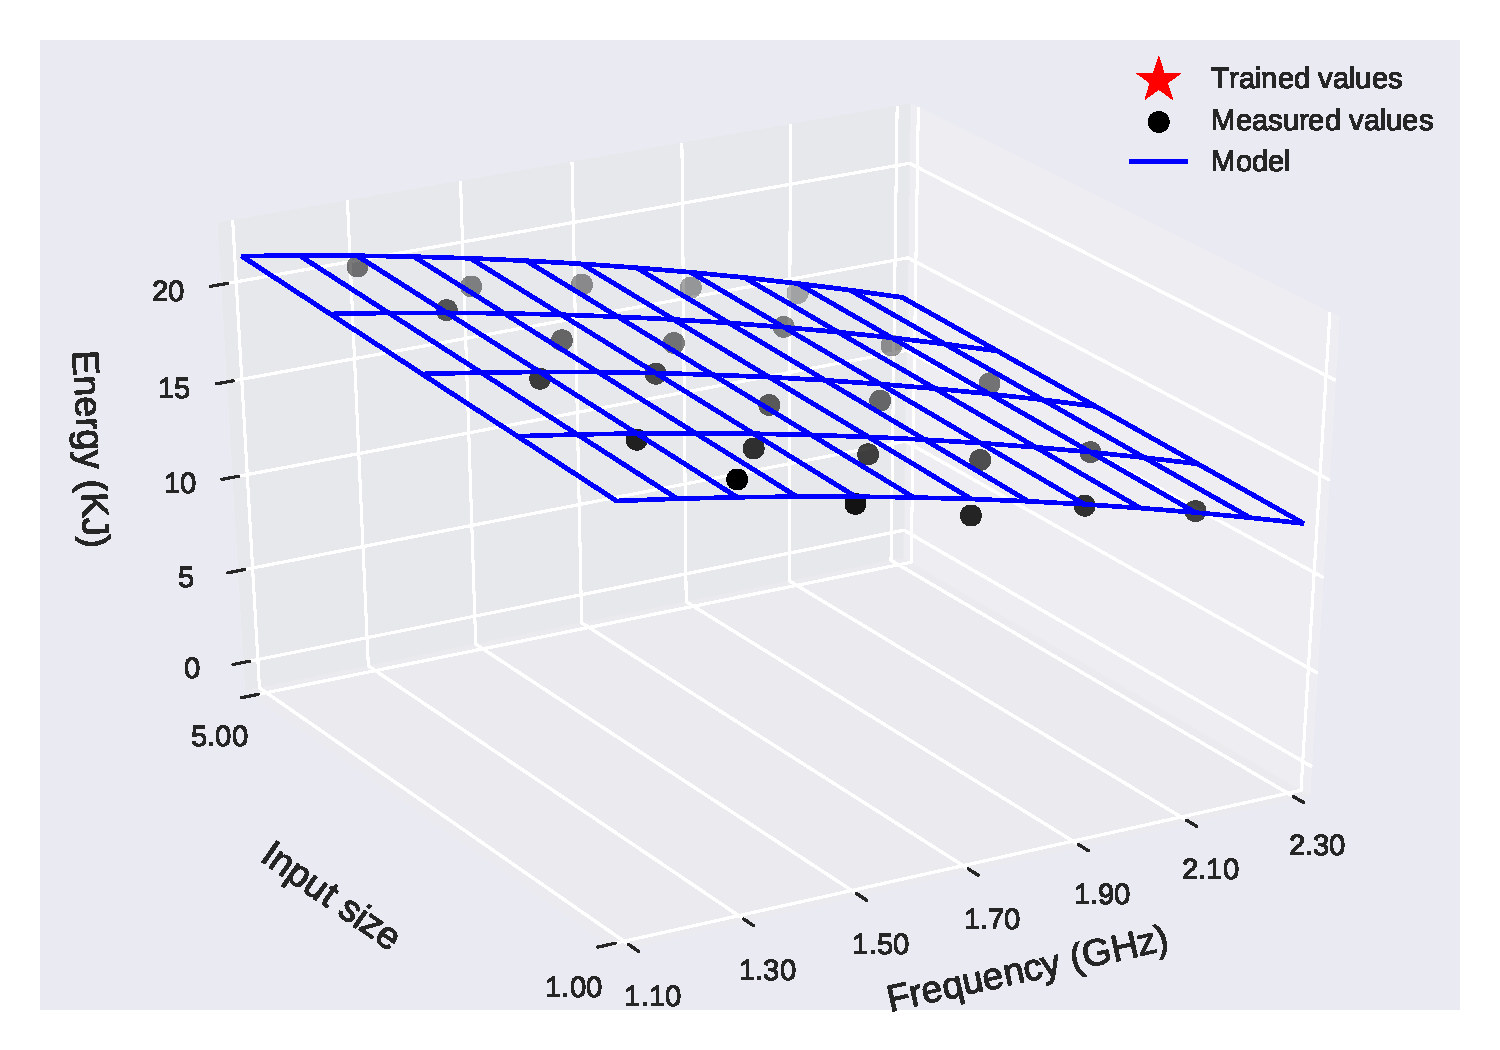
\includegraphics[width=\columnwidth]{models/figures/energy/freq_inps/completo_canneal_1.pdf}}
		\caption{}
		\label{fig:en_eq_canneal_fi}
	\end{subfigure}
	
	\caption{Example fit for a specific input size: Blackscholes (\textbf{a}) and Canneal (\textbf{b}).  “measured values” are the sensor data and “minimum energy” is the minimum energy model prediction.
	}
	\label{fig:en_eq_freq_inp_fi}
\end{figure}
\subsubsection{Cores $\times$ Input}
\cref{fig:en_eq_core_inp_ci} plots the measured and modeled energy consumption for some of the applications modeled. The diagrams  show some of the possible shapes that the model can take while varying the number of active cores, and input size.
\begin{figure}[H]
	\centering
	\captionsetup[subfigure]{justification=centering}
	\begin{subfigure}[b]{0.45\textwidth}
		\centerline{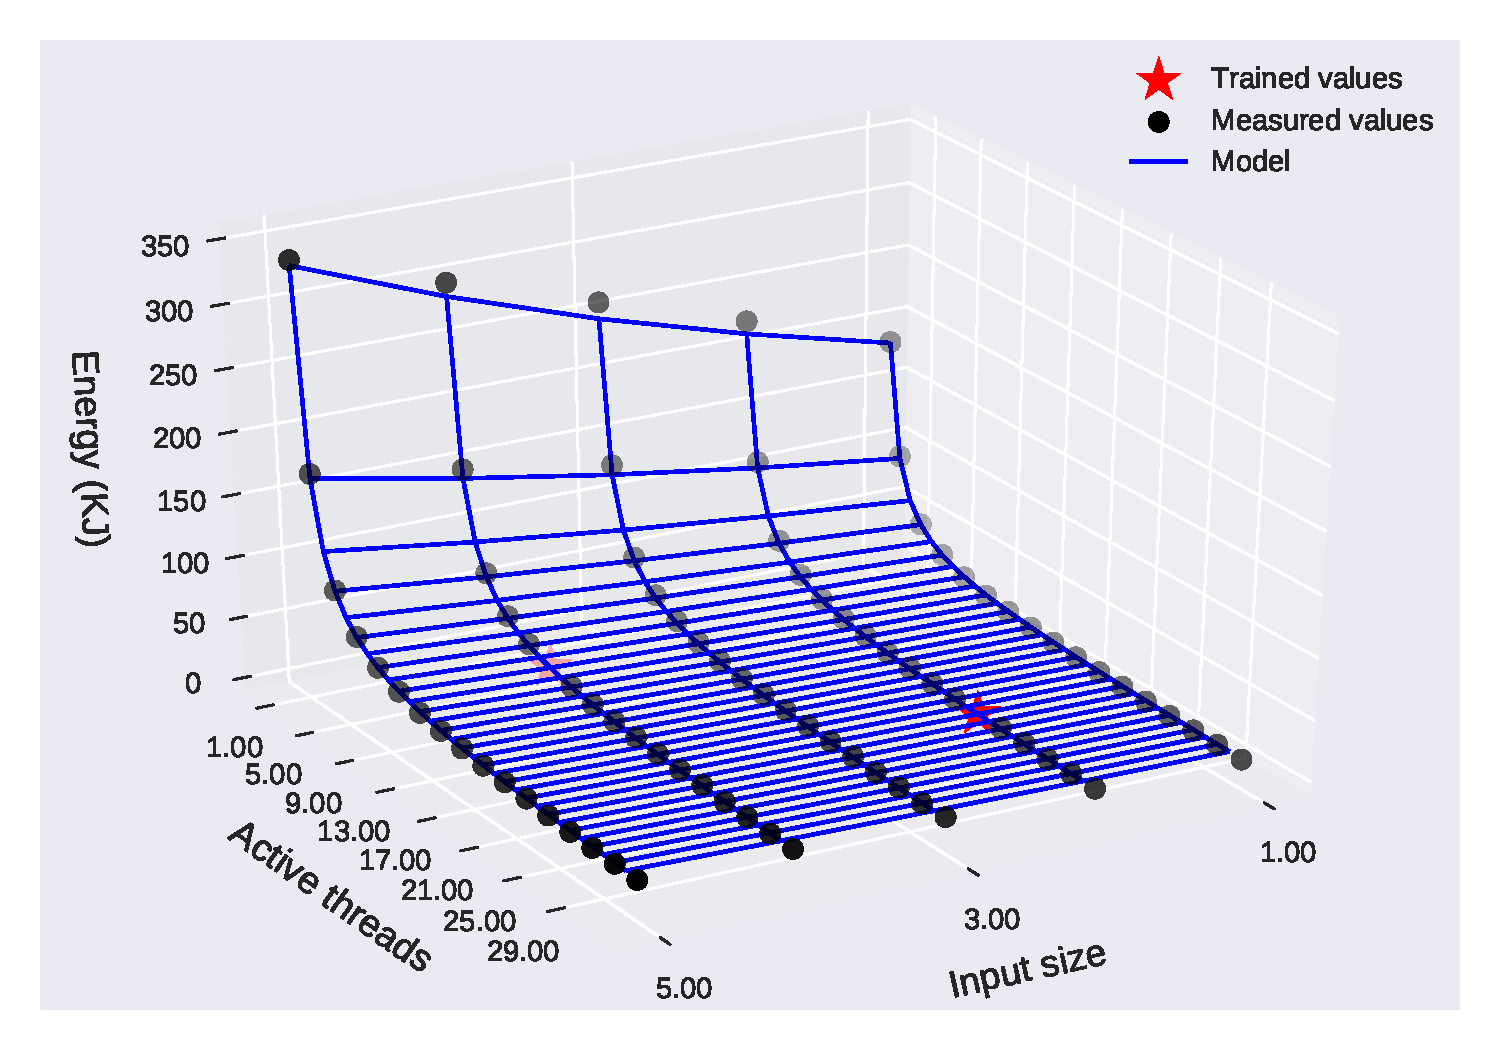
\includegraphics[width=\columnwidth]{models/figures/energy/cores_inps/completo_black_5.pdf}}
		\caption{}
		\label{fig:en_eq_black_ci}
	\end{subfigure}
	%
	\begin{subfigure}[b]{0.45\textwidth}
		\centerline{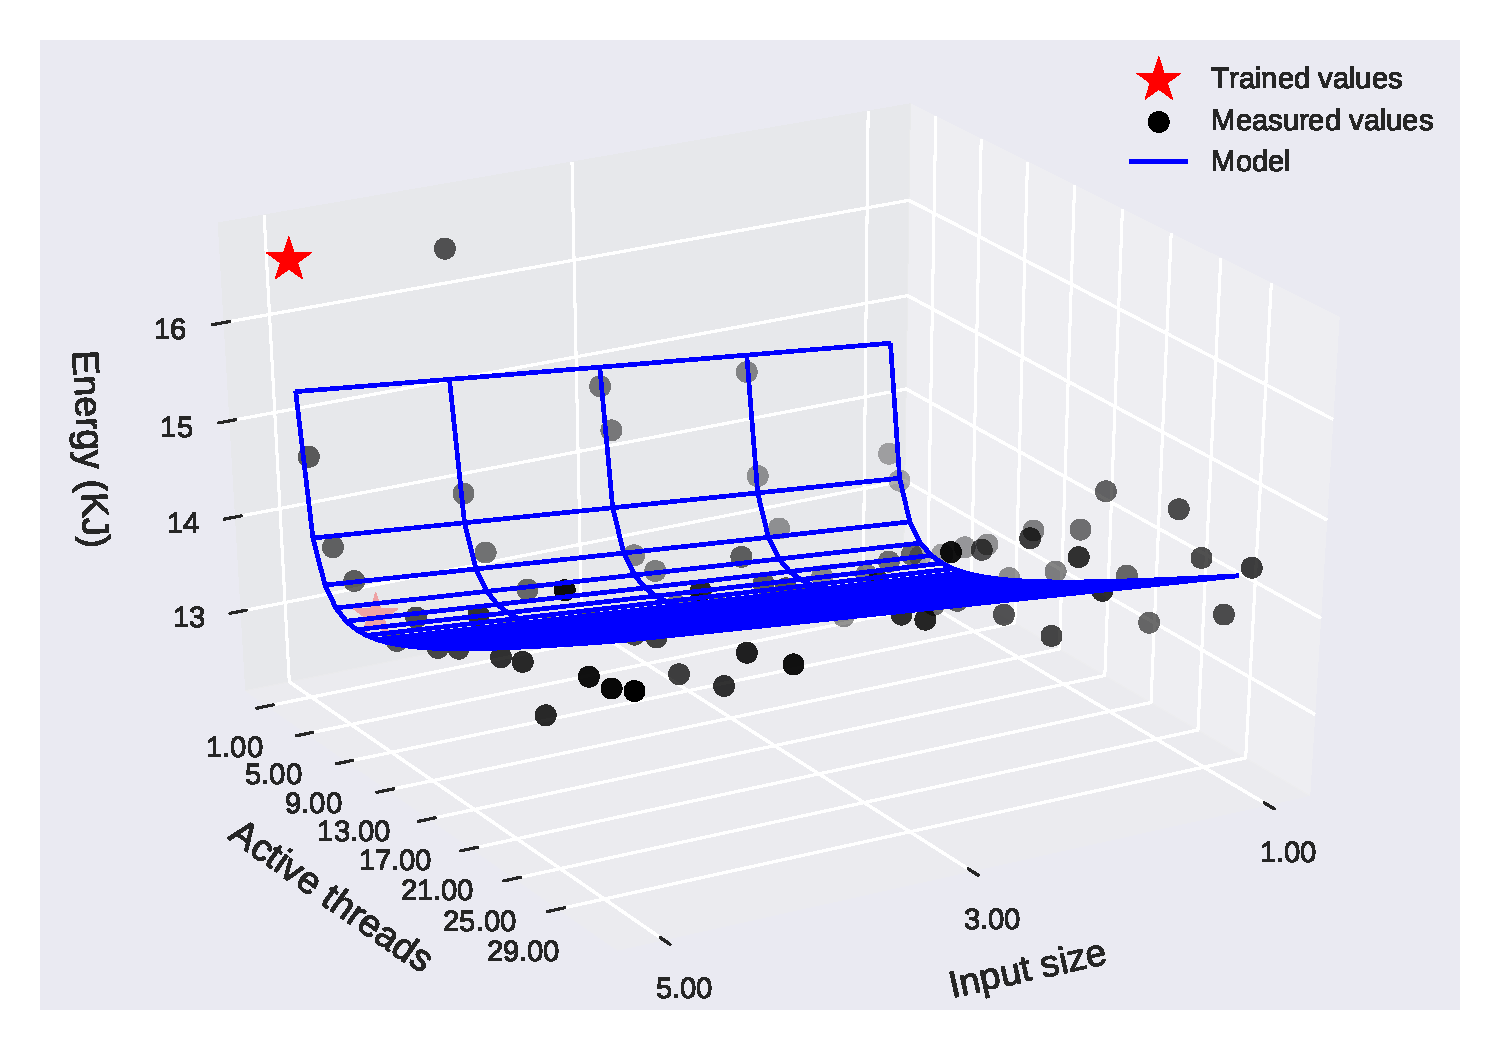
\includegraphics[width=\columnwidth]{models/figures/energy/cores_inps/completo_canneal_1.pdf}}
		\caption{}
		\label{fig:en_eq_canneal_ci}
	\end{subfigure}
	
	\caption{Example fit for a specific input size: Blackscholes (\textbf{a}) and Canneal (\textbf{b}).  “measured values” are the sensor data and “minimum energy” is the minimum energy model prediction.
	}
	\label{fig:en_eq_core_inp_ci}
\end{figure}


\subsubsection{Comparison}
The average results for each application were calculated using a model trained with only 10 configurations, and the comparison is displayed \cref{fig:mpe_svr_eq}. %We calculated the raw MPE values shown in ~\cref{tab:mpe_svr_eq}.
\begin{figure}[H]
	\centering
	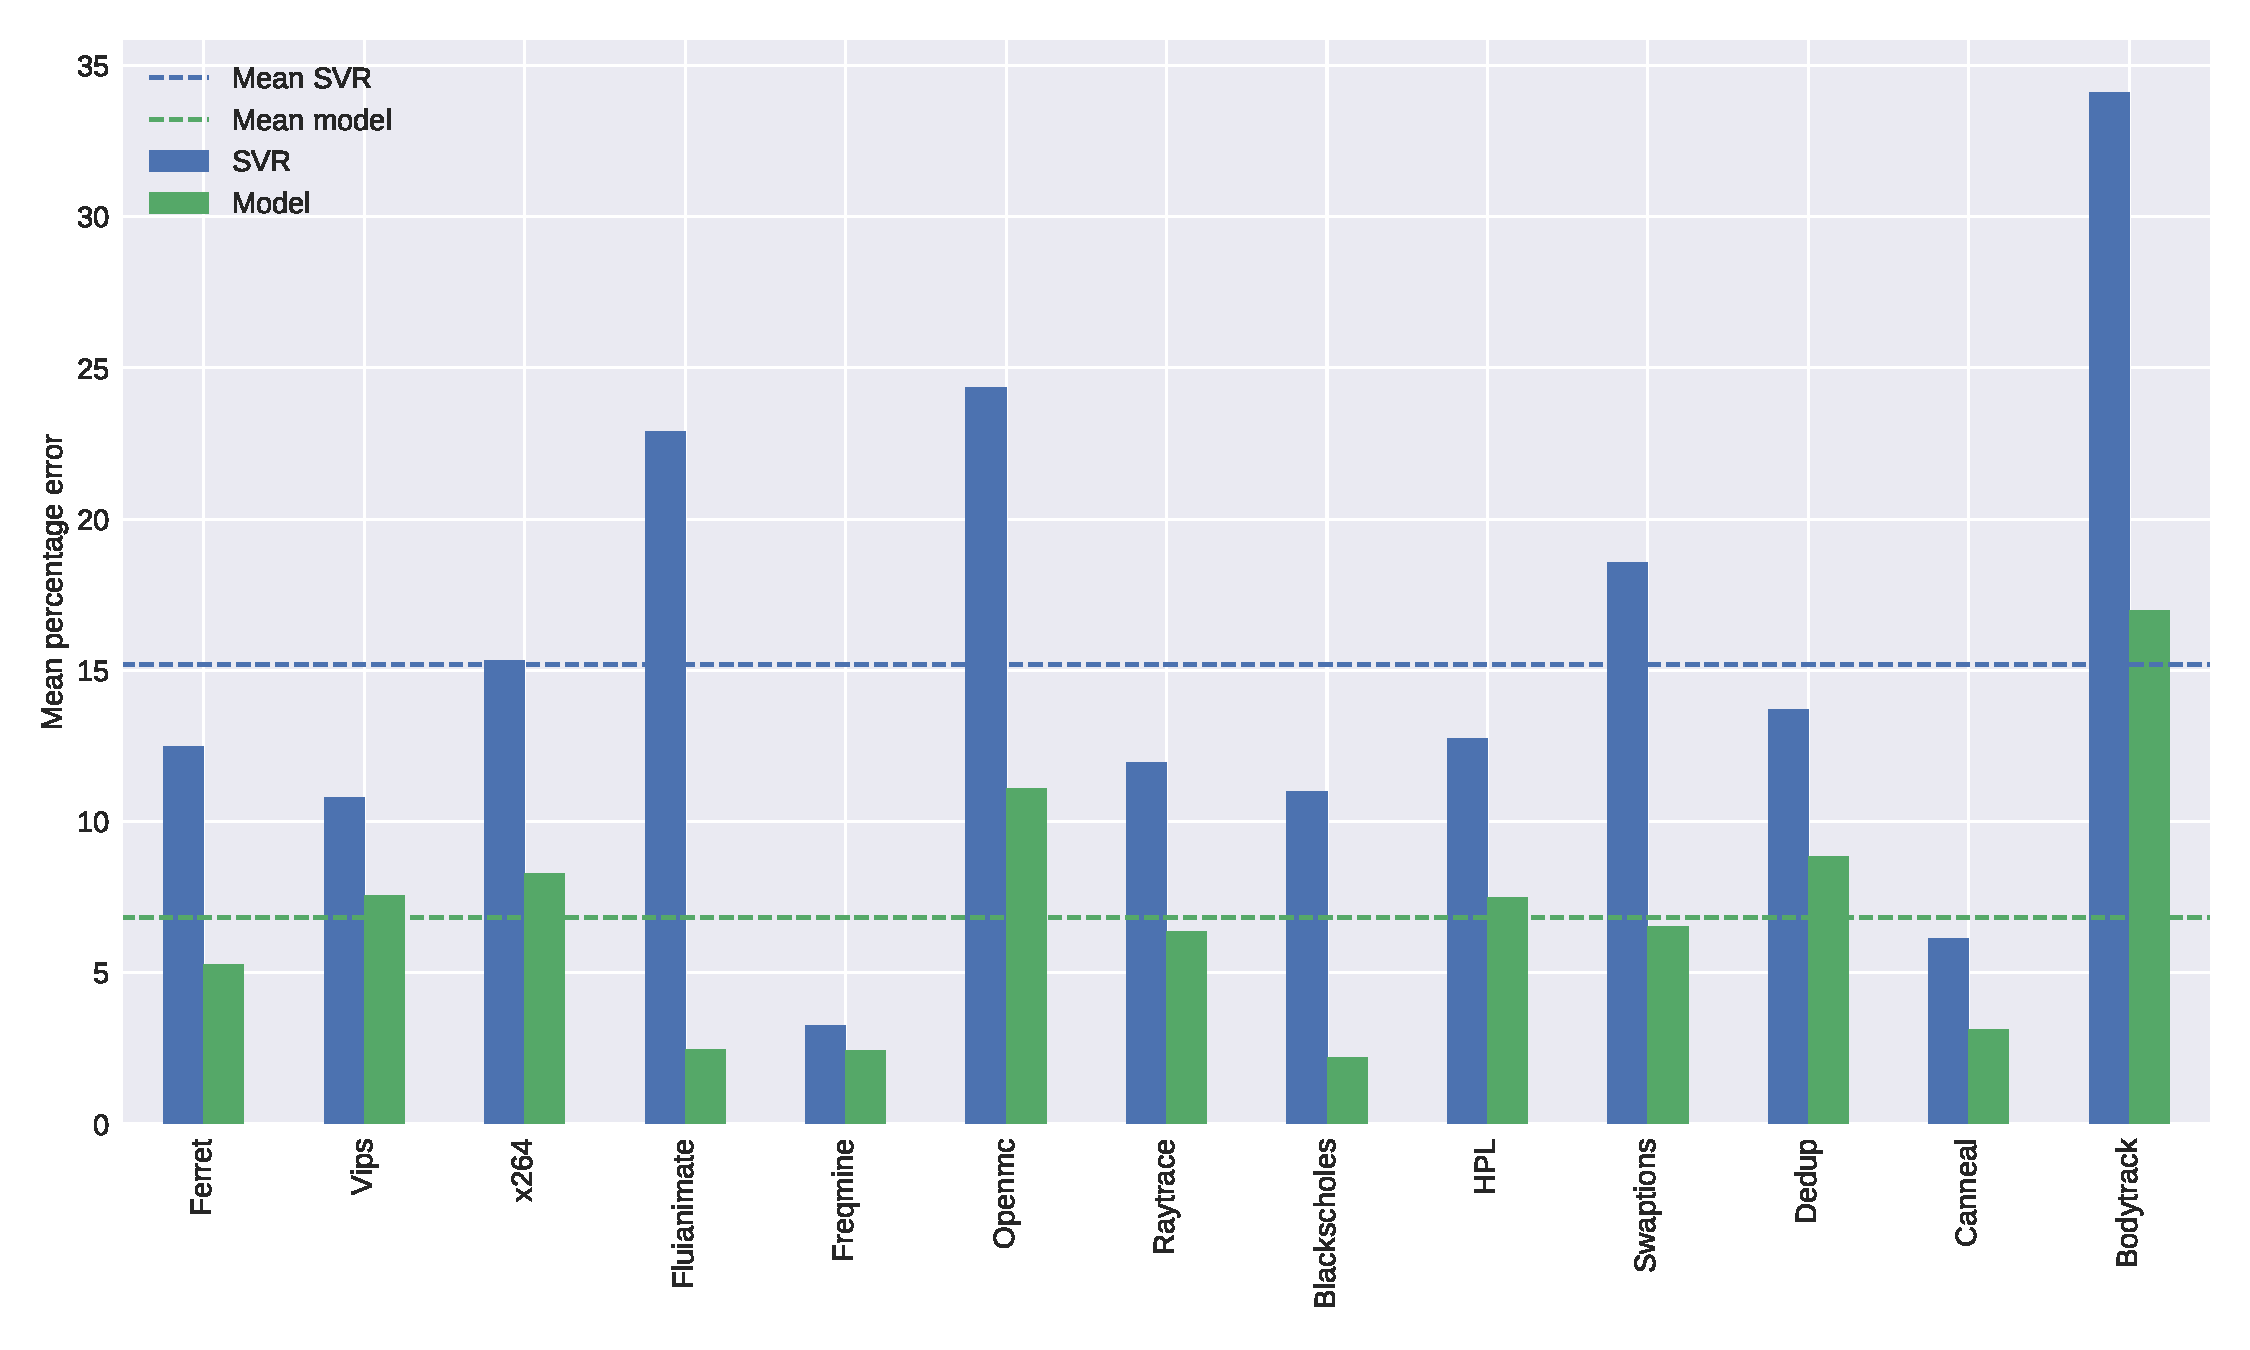
\includegraphics[width=.8\columnwidth]{models/figures/mpe_svr_eq.pdf}
	\caption{Comparison of the mean percentage error between the proposed model and SVR. ``Model mean'' and ``SVR mean'' are the average of all MPE values for all applications.
	}
	\label{fig:mpe_svr_eq}
\end{figure}

\cref{fig:mpe_svr_eq} shows that the proposed model always performed better, with a lower MPE than SVR, when we were limited to 10 training points. This result is further explored in the next Section \ref{subsec:overhead}, where we undertake a comparison with different training sizes. The exact values are shown in \cref{tab:mpe_svr_eq}.

\begin{table}[H]
\centering
\begin{tabular}{c|c|c}
\hline
Application  & Model & SVR   \\ \hline
Ferret       & 5.25     & 12.49  \\ 
Raytrace     & 6.36     & 11.95  \\
Fluianimate  & 2.44     & 22.90  \\
x264         & 8.28     & 15.33  \\
Vips         & 7.54     & 10.80  \\
Swaptions    & 6.54     & 18.57  \\
Canneal      & 3.12     & 6.13   \\
Dedup        & 8.85     & 13.70  \\
Freqmine     & 2.44     & 3.24   \\
Blackscholes & 2.18     & 11.00  \\
HPL          & 7.47     & 12.75  \\
Bodytrack    & 16.98    & 34.12  \\
Openmc       & 11.15    & 24.34  \\
\end{tabular}
\caption{Comparison of the Mean Percentage Error between the proposed model and SVR: raw values.}
\label{tab:mpe_svr_eq}
\end{table}

\subsection{Overheads on Training} \label{subsec:overhead}
It is known that machine learning is data-driven; in that sense, the SVR model obtained using only 10 configurations could be improved, but what about the analytical model? 
To answer that question, the proposed model and the SVR were also trained with a varying number of configurations.
We then compared the MPE and the amount of energy spent to create each model. 
This accuracy-energy trade-off is crucial since building models' energy overhead defeats the primary goal of saving power when running applications.
\enlargethispage{.5cm}

\begin{figure}[H]
	\centering
	\captionsetup[subfigure]{justification=centering}
	\begin{subfigure}[b]{0.45\textwidth}
		\centerline{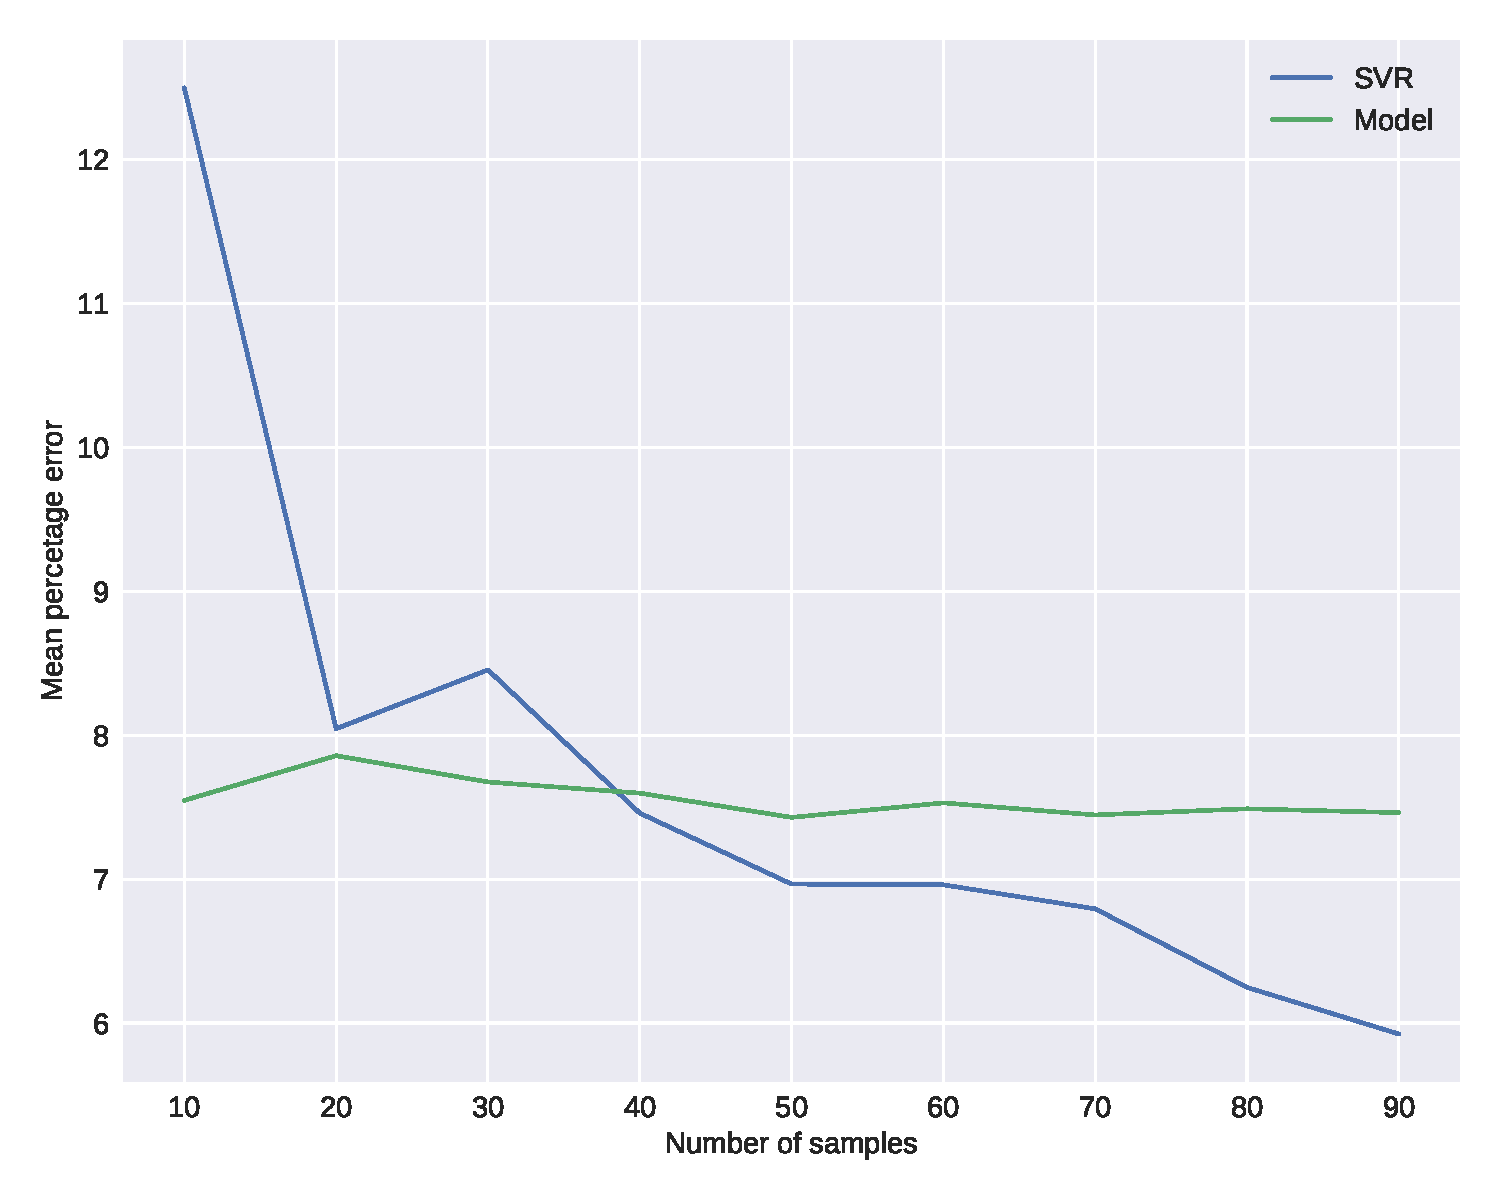
\includegraphics[width=\columnwidth]{models/figures/overhead/completo_ferret_4.pdf}}
		\caption{MPE for Ferret.}
		\label{fig:overhead_ferret}
	\end{subfigure}
	%
	\begin{subfigure}[b]{0.45\textwidth}
		\centerline{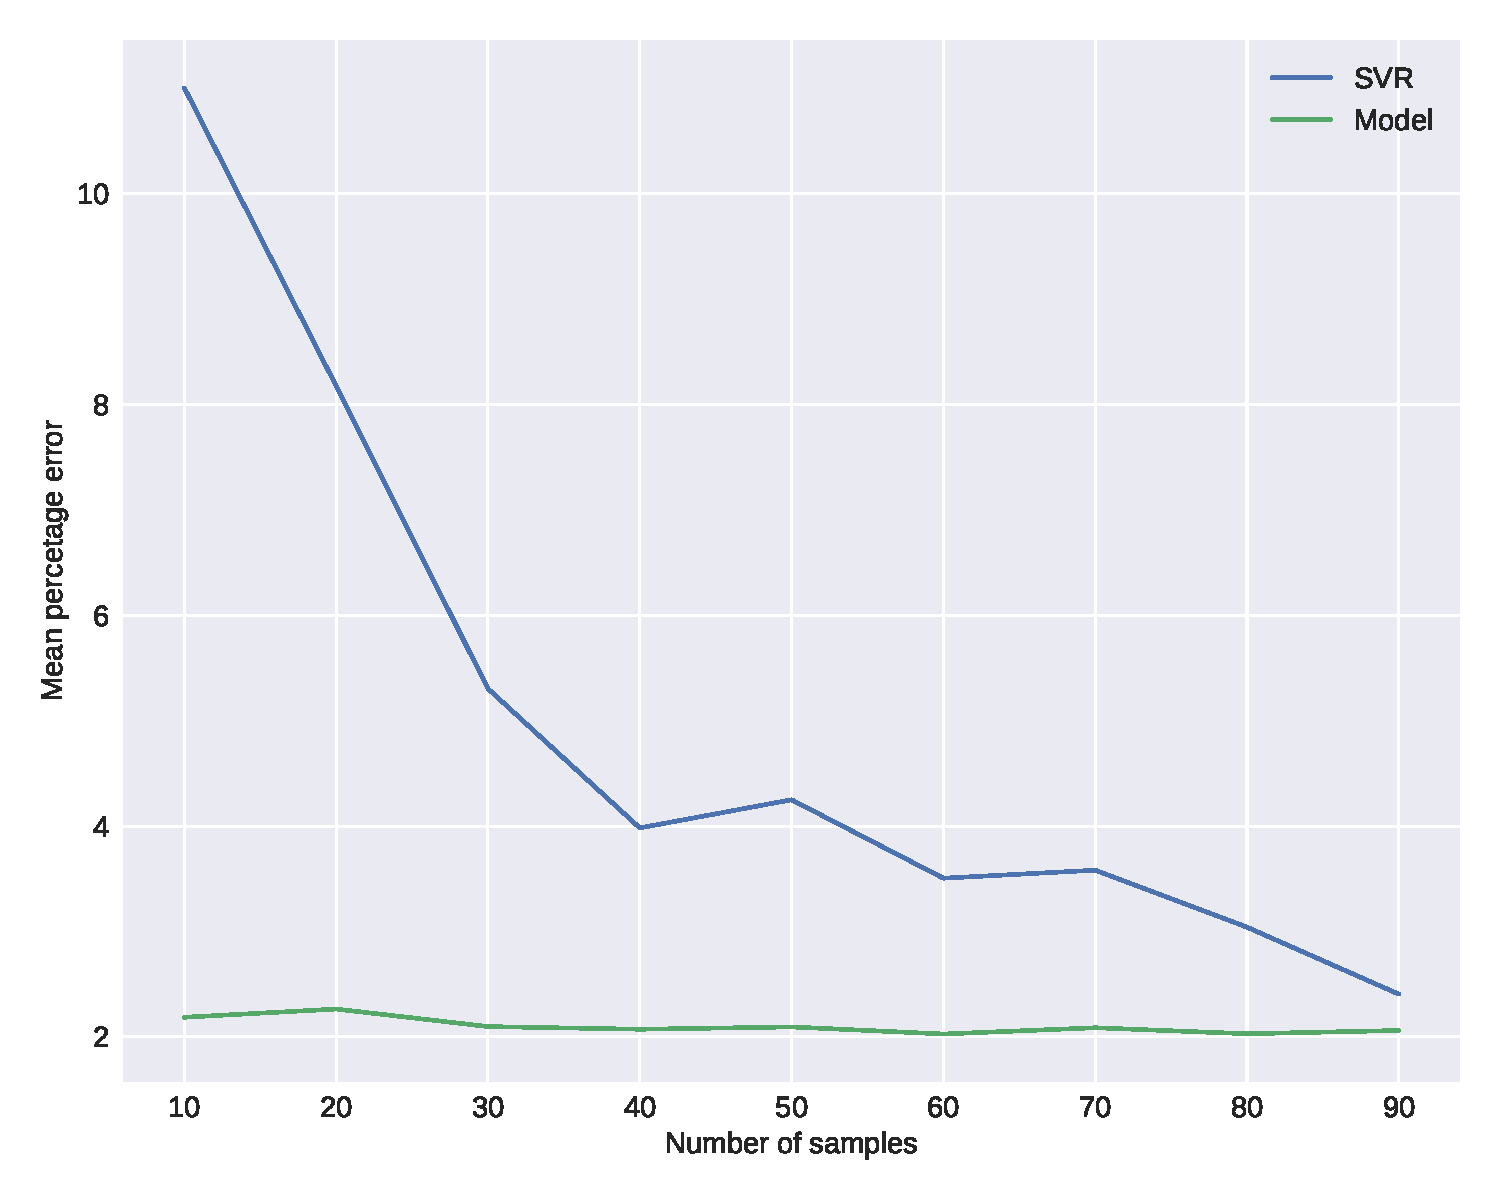
\includegraphics[width=\columnwidth]{models/figures/overhead/completo_black_6.pdf}}
		\caption{MPE for Blackscholes.}
		\label{fig:overhead_black}
	\end{subfigure}
	%
	\par\bigskip
	\begin{subfigure}[b]{0.45\textwidth}
		\centerline{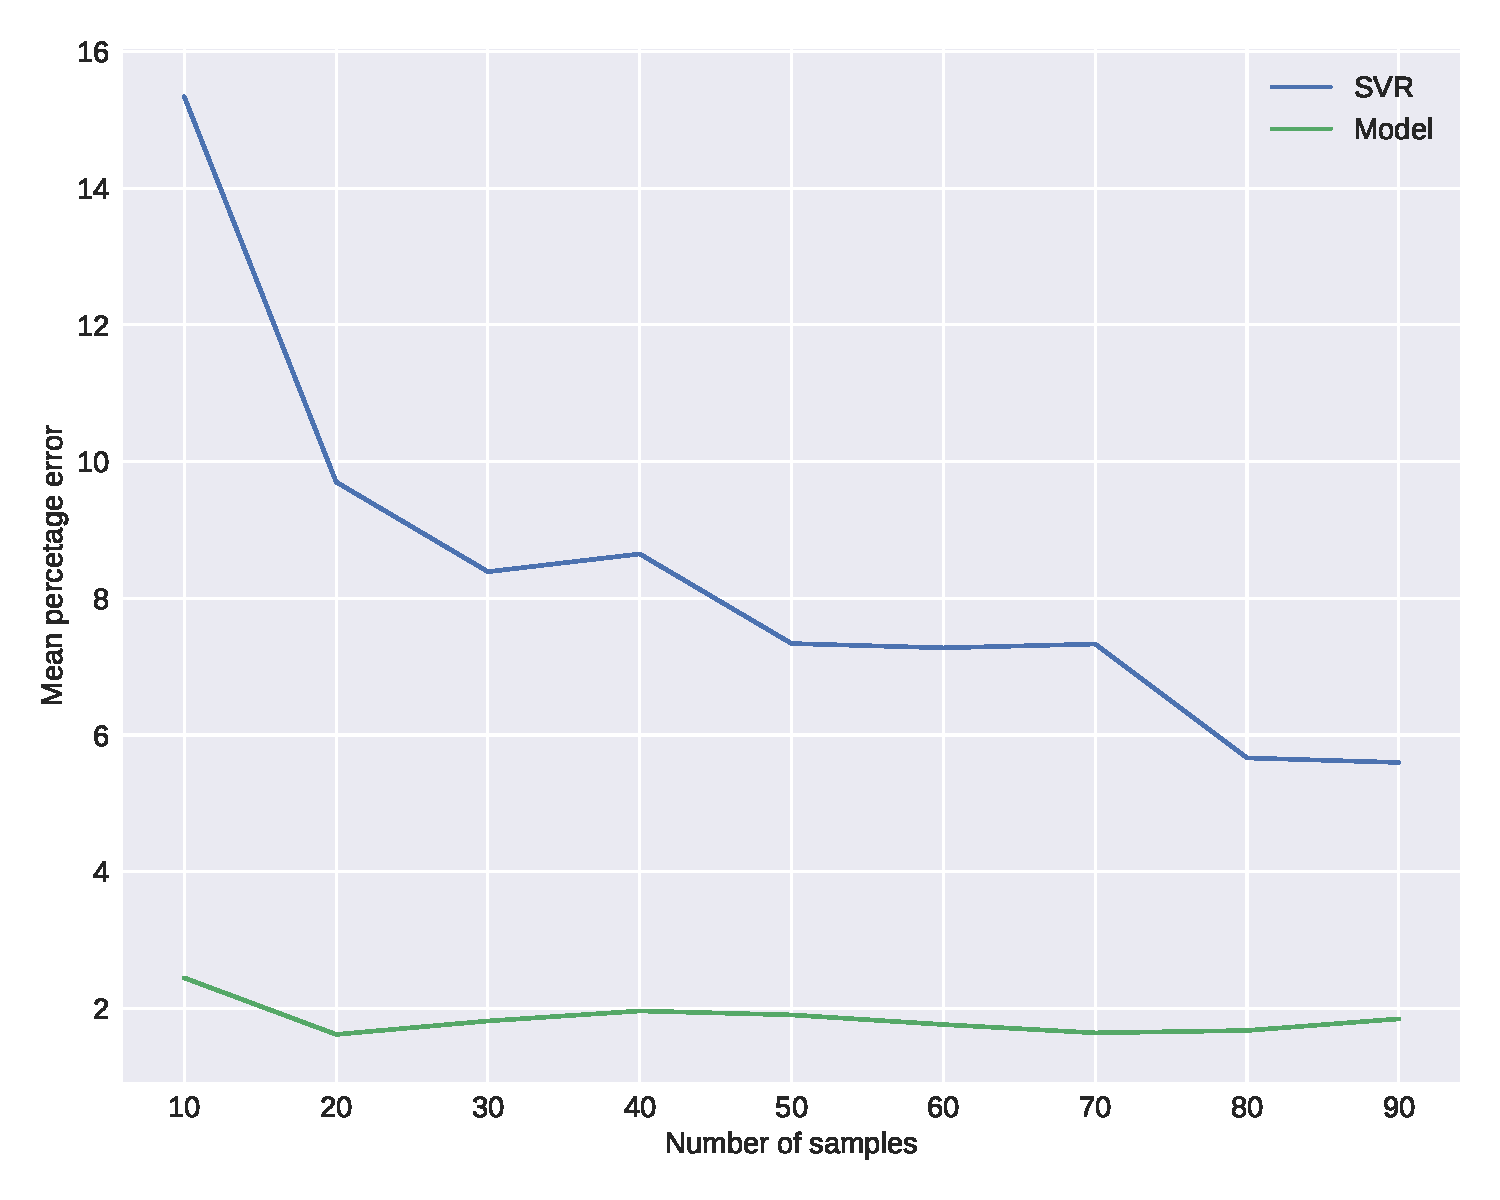
\includegraphics[width=\columnwidth]{models/figures/overhead/completo_x264_4.pdf}}
		\caption{MPE for x264.}
		\label{fig:overhead_x264}
	\end{subfigure}
	%
	\begin{subfigure}[b]{0.45\textwidth}
		\centerline{\includegraphics[width=\columnwidth]{models/figures/overhead/completo_dedup_4.pdf}}
		\caption{MPE for Dedup.}
		\label{fig:overhead_dedup}
	\end{subfigure}
	
	\caption{MPE of the case studies versus training size, comparing how many training points is necessary to reach an acceptable result.}
	\label{fig:overheadapps}
\end{figure}

\cref{fig:overheadapps} shows the comparisons of MPE and energy spent to create each model for two selected applications. According to the results, the analytical model is very stable, not changing much as more data is added, while the SVR keeps reshaping to adapt to the data. 
The error of the analytical model is almost constant but that of the SVR, initially very high, drops as more data is used in the training process.
\begin{figure}[H]
	\centering
	\captionsetup[subfigure]{justification=centering}
	\begin{subfigure}[t]{0.45\textwidth}
		\includegraphics[width=\columnwidth]{models/figures/overhead/overall_energy_10pts.pdf}
		\caption{}
		\label{fig:overall_overhead}
	\end{subfigure}
	%
	%\par\bigskip
	\begin{subfigure}[t]{0.45\textwidth}
		\includegraphics[width=\columnwidth]{models/figures/overhead/overall_mpe_10pts.pdf}
		\caption{
		}
		\label{fig:overall_MPE}
	\end{subfigure}
	\caption{Overall results for energy and MPE for each training size. (\textbf{a}) Average energy spent on all applications during model creation. The two curves are identical because the same data were used to adjust the SVR and the model. (\textbf{b}) MPE of all applications: SVR needs 10 times more data to have an MPE lower than the proposed model.}
	\label{fig:overall_train}
\end{figure}

\cref{fig:overall_train} presents the overall results, with the mean energy overhead and MPE for all applications.
The meeting point of the MPE for the SVR and the proposed model can be extracted from \cref{fig:overall_train}b.
It shows that, in around 90 configurations, the SVR starts to have a smaller error. The cost of that is the linear increase in energy spent on training. The increase in energy, about 10 times more, can be observed in \cref{fig:overall_train}a.

\subsection{Analysis}
One of the most significant advantages of using an analytical model is the understanding of the problem that an equation provides, making many different kinds of analysis possible that are otherwise impossible with a machine learning model. In this section, we discuss one of the possible analyses. In the following figures, we try to understand the contribution of each parameter of the equation to the total energy consumption.

For this analysis, we took the model of one of the applications and, varying one parameter of the equation, we display the energy versus performance (time) for all configurations. After that, we computed the Pareto frontier, a set of all Pareto efficient allocations, i.e., all the configurations where resources cannot be reallocated to make one individual better off without making at least one individual worse off. This gives us all the configurations where we have an optimal trade-off of performance and energy to choose from.


\cref{fig:pareto_static} shows the Pareto frontier for several values for the static power parameter ($c_3$ in \cref{eq:en_final}) with configurations of frequency ranging from 1.2 to 5 GHz and cores from 1 to 64, so that we can also have an idea of what is the tendency when we increase the frequency and number of cores.

\begin{figure}[H]
	\includegraphics[width=\columnwidth]{models/figures/analisys/pareto_static_high.pdf}
	\caption{Pareto frontier for several values of static power parameter. The arrows with blue heads indicate the maximum energy, while the arrows with a red head the minimal energy for each corresponding curve.}% In four-digit numbers, no comma or spaces to indicate thousand, whatever the numbers are in the table or body text, e.g., 4500; More than five-digit numbers, should have comma, e.g. 59,400; 899,302. Please revise the figure.
	\label{fig:pareto_static}
\end{figure}
%Fixed

From this figure, we can see that when increasing the value of the static power parameter, the total energy consumption increases as expected. We can also observe that the values that minimize the total energy consumption tend to be high frequency and multiple cores. This is one of the consequences of increasing the static power factor. As the dynamic factor proportionally decreases, its variables tend to have less impact on total consumption, enabling configurations with high frequency and several cores. This also enables chip-level optimization for choosing components that change the ratio between static and dynamic power.


\cref{fig:pareto_w} shows the Pareto frontier in the same ranges described before but for the parameter corresponding to the level of parallelism of the application ($w$ in  \cref{eq:en_final}).

\begin{figure}[H]
	\includegraphics[width=\columnwidth]{models/figures/analisys/pareto_w_high.pdf}
	\caption{Pareto frontier for several values of static power parameter. The arrows with blue heads indicate the maximum energy, while the arrows with a red head, the minimal, for each corresponding curve.}% In four-digit numbers, no comma or spaces to indicate thousand, whatever the numbers are in the table or body text, e.g., 4500; More than five-digit numbers, should have comma, e.g. 59,400; 899,302. Please revise the figure.
	\label{fig:pareto_w}
\end{figure}
%Fixed

In  \cref{fig:pareto_w}, we observe that, as the parallelism level increases the total energy decreases. The number of cores tends to be higher with a higher level of parallelism as expected, and the frequency shows an inverse relation.


\subsection{DVFS and DPM Optimization} \label{subsec:dvfs_optmin}
The effectiveness of the proposed approach during optimization was evaluated with a simple algorithm that finds the optimal frequency and number of active cores from the proposed equation. The results were then compared to the Linux default choices for power management.

With \cref{eq:en_final}, it is possible to calculate energy consumption estimates for each possible configuration since there is a finite range of possible values for the frequency and number of cores. It is also possible to apply constraints on the execution time, frequency, and the number of active cores. Then, the configuration that minimizes energy consumption for a given input can be selected. The complete workflow is shown in \cref{fig:optim_workflow}. We can see that any optimization problem can be structured with our model and the system's constraints. In the following examples, the optimization problem that we build is to minimize the energy equation given the constraints of possible frequencies and the number of cores that our system can run. The algorithm selected to minimize was the newton-CG~\cite{Royer2020AOptimization}.

Current HPC managers leave to the user the choice of how many cores to use. On this basis, three situations were analyzed in relation to the number of cores:

\begin{enumerate}
	\item Worst choice: number of cores that maximize the total energy consumed;
	\item Random choice: energy consumed for a random choice of the number of cores;
	\item Best choice: number of cores that minimize the total energy consumed (oracle).
\end{enumerate}
\begin{figure}[H]
	\centering
	\includegraphics[width=0.8\columnwidth]{models/figures/DVFS optim.pdf}
	\caption{Optimization workflow showing how DVFS and DPM optimization could be implemented from ou model.}
	\label{fig:optim_workflow}
\end{figure}


The default option for the Linux governor is Ondemand, and, by default, it has no DPM control for the number of active cores. As Ondemand only performs DVFS, \textls[-15]{for comparison, each application was executed with all available cores in the system, from 1 to 32.}

\textls[-15]{Figures \ref{fig:energy_worst_case}--\ref{fig:energy_best_case}, show the energy savings with respect to Ondemand, i.e., $\frac{Ondemand-Model_{min}}{Ondemand}$} for the three cases described above. The savings and losses for each case are:

\begin{enumerate}
	\item Worst choice: save 69.88\% on average;
	\item Random choice: save 12.04\% on average;
	\item Best choice: lost 14.06\% on average.
\end{enumerate}

\begin{figure}[H]
	\centering
	\includegraphics[width=\columnwidth]{models/figures/dvfs_cmp_max.pdf}
	\caption{Energy savings comparisons between the proposed model and the Worst case.}
	\label{fig:energy_worst_case}
\end{figure}

\begin{figure}[H]
	\centering
	\includegraphics[width=\columnwidth]{models/figures/dvfs_cmp_mean.pdf}
	\caption{Energy savings comparisons between the proposed model and the Random case.}
	\label{fig:energy_mean_case}
\end{figure}

By default, operating systems do not implement DPM at the core level, and, in HPC, the user usually explicitly chooses the number of cores to run their job. To give a better idea of the impact on the energy consumption of DPM at the core level, we analyzed the choices of the number of cores over a period of one year in the HPC center at UFRN. The result is plotted in~\cref{fig:cpu_requests}.


It is of note that the most common choice of many regular users is a single core requested per job, matching the worst-case choice for all applications analyzed in this investigation. The best choice was quite often 32 cores, which is the third most popular choice among users, but it is 72 times less frequent than 1 core. This led us to envision how much energy could be saved and encouraged us towards future research using the proposed model for DPM or more advanced optimization algorithms.

In practice, this approach can be implemented by allowing the resource manager to perform these changes for the user using pre-scripts and post-scripts for high energy consumption job submissions.
\begin{figure}[H]
	\centering
	\includegraphics[width=\columnwidth]{models/figures/dvfs_cmp_32.pdf}
	\caption{Energy savings comparisons between the proposed model and the Best case.}
	\label{fig:energy_best_case}
\end{figure}
\vspace{-12pt}

\begin{figure}[H]
	\centering
	\includegraphics[width=\columnwidth]{experiments/figures/cpu_requestes.pdf}
	\caption{Number of CPU requests during one year in HPC cluster, sorted by the number of cores requested per job.}
	\label{fig:cpu_requests}
\end{figure}

%\section{PMCs}
%
%\section{Energy per instruction}
%
%\begin{lstlisting}
%xor rcx, rcx
%mov rax, 1
%mov rdx, 0
%
%loop:
%	targ_inst(*arg)
%	targ_inst(*arg)
%	targ_inst(*arg)
%	targ_inst(*arg)
%	targ_inst(*arg)
%	targ_inst(*arg)
%	targ_inst(*arg)
%	targ_inst(*arg)
%	targ_inst(*arg)
%
%add rcx, 1
%cmp rcx, 9999999
%jne loop
%\end{lstlisting}
%
%Estimating the energy of the instruction from this benchmark
%
%$E_{total}=9999999(\frac{10}{13}inst+\frac{3}{13}loop)$
%
%$E_{total}=7692306*inst+constant$
%
%\subsection{Generic}
%
%\begin{figure}
%	\centering
%	\includegraphics[width=\textwidth]{experiments/figures/inst_en_args_generic.png}
%	\caption{Energy per instruction argument}
%	\label{fig:experiment_en1}
%\end{figure}
%
%\begin{figure}
%	\centering
%	\includegraphics[width=\textwidth]{experiments/figures/inst_mean_en_generic.png}
%	\caption{Mean energy per instruction over all arguments}
%	\label{fig:experiment_en2}
%\end{figure}
%
%\begin{figure}
%	\centering
%	\includegraphics[width=\textwidth]{experiments/figures/inst_std_en_generic.png}
%	\caption{Standard deviation energy per instruction over all arguments}
%	\label{fig:experiment_en3}
%\end{figure}
%
%\subsection{SSE}
%
%\begin{figure}
%	\centering
%	\includegraphics[width=\textwidth]{experiments/figures/inst_en_args_sse.png}
%	\caption{Energy per instruction argument (sse)}
%	\label{fig:experiment_en4}
%\end{figure}
%
%\begin{figure}
%	\centering
%	\includegraphics[width=\textwidth]{experiments/figures/inst_mean_en_sse.png}
%	\caption{Mean energy per instruction over all arguments (sse)}
%	\label{fig:experiment_en5}
%\end{figure}
%
%\begin{figure}
%	\centering
%	\includegraphics[width=\textwidth]{experiments/figures/inst_std_en_sse.png}
%	\caption{Standard deviation energy per instruction over all arguments (sse)}
%	\label{fig:experiment_en6}
%\end{figure}
%
%\subsection{SSE and Generic}
%
%\begin{figure}
%	\centering
%	\includegraphics[width=\textwidth]{experiments/figures/inst_en_cmp_sse_generic.png}
%	\caption{Comparing SSE and generic instructions energy consumption}
%	\label{fig:experiment_en7}
%\end{figure}
%
%\subsection{Power}
%
%\begin{figure}
%	\centering
%	\includegraphics[width=\textwidth]{experiments/figures/inst_pw_generic.png}
%	\caption{Instructions power draw}
%	\label{fig:experiment_pw1}
%\end{figure}
%\begin{figure}
%	\centering
%	\includegraphics[width=\textwidth]{experiments/figures/inst_pw_args.png}
%	\caption{Instructions power draw by argument}
%	\label{fig:experiment_pw2}
%\end{figure}
%
%\section{Tracing application methods}
%
%\begin{outline}
%	\1 Linux ptrace
%		\2 Breakpoint on each instruction	
%	\1 Intel pin
%		\2 JIT
%		\2 Not open source
%	\1 qemu user
%		\2 TCG accelerator (transform target to host instruction) similar to JIT
%		\2 Partial emulation
%\end{outline}
%
%We choose the less intrusive and open-source alternative qemu user, with an small modificaion we are able to trace an application instructions. Generating an table as follows:
%
%
%\begin{table}[H]
%	\centering
%	\begin{tabular}{|c|c|c|}
%		\hline
%		opcode         & mnemonic & args                          \\ \hline
%		48 89 e7       & movq     & \%rsp, \%rdi\textbackslash{}n \\ \hline
%		48 89 e7       & movq     & \%rsp, \%rdi\textbackslash{}n \\ \hline
%		e8 08 0e 00 00 & callq    & 0x4000a24ea0\textbackslash{}n \\ \hline
%		55             & pushq    & \%rbp\textbackslash{}n        \\ \hline
%		48 89 e5       & movq     & \%rsp, \%rbp\textbackslash{}n \\ \hline
%		41 57          & pushq    & \%r15\textbackslash{}n        \\ \hline
%		41 56          & pushq    & \%r14\textbackslash{}n        \\ \hline
%		41 55          & pushq    & \%r13\textbackslash{}n        \\ \hline
%		& \vdots & \\ \hline
%	\end{tabular}
%\end{table}
%
%
%\section{CPU load}
%
%\begin{figure}[H]
%	\centering
%	\begin{subfigure}[b]{0.45\textwidth}
%		\centering
%		\includegraphics[width=1\columnwidth]{experiments/figures/pw_freq_load.png}
%		\caption{Instructions power draw varing CPU load}
%		\label{fig:experiment_pw_load}
%	\end{subfigure}
%	%
%	\begin{subfigure}[b]{0.45\textwidth}
%		\centering
%		\includegraphics[width=1\columnwidth]{experiments/figures/pw_load.png}
%		\caption{Instructions power draw varing CPU load}
%		\label{fig:experiment_pw_load}
%	\end{subfigure}
%\end{figure}
%
%
%\section{Analysis}
%
%\subsection{Pareto points}

%
%\begin{figure}

%	\centering

%	\includegraphics[width=\columnwidth]{models/figures/analisys/pareto_static_high.png}

%	\caption{Pareto static energy}

%	\label{fig:pareto_static_h}

%\end{figure}

%
%
%\begin{figure}

%	\centering

%	\includegraphics[width=\columnwidth]{models/figures/analisys/pareto_static_low.png}

%	\caption{Pareto static energy}

%	\label{fig:pareto_static_l}

%\end{figure}

%
%
%\begin{figure}

%	\centering

%	\includegraphics[width=\columnwidth]{models/figures/analisys/pareto_w_high.png}

%	\caption{Pareto w energy}

%	\label{fig:pareto_w_h}

%\end{figure}

%
%\begin{figure}

%	\centering

%	\includegraphics[width=\columnwidth]{models/figures/analisys/pareto_static_low.png}

%	\caption{Pareto w energy}

%	\label{fig:pareto_w_l}

%\end{figure}

%
%\subsection{Optimization under constraints}

%
%\subsection{Gradient and Countorns}

%
%\begin{figure}[H]

%	\centering

%	\begin{subfigure}[b]{0.45\textwidth}

%		\includegraphics[width=\textwidth]{models/figures/analisys/pdyn0.png}

%	\end{subfigure}

%	%

%	\begin{subfigure}[b]{0.45\textwidth}

%		\includegraphics[width=\textwidth]{models/figures/analisys/pdyn0_3d.png}

%	\end{subfigure}

%\end{figure}

%
%\begin{figure}[H]

%	\centering

%	\begin{subfigure}[b]{0.45\textwidth}

%		\includegraphics[width=\textwidth]{models/figures/analisys/pdyn3.png}

%	\end{subfigure}

%	%

%	\begin{subfigure}[b]{0.45\textwidth}

%		\includegraphics[width=\textwidth]{models/figures/analisys/pdyn3_3d.png}

%	\end{subfigure}

%\end{figure}

%
%\begin{figure}[H]

%	\centering

%	\begin{subfigure}[b]{0.45\textwidth}

%		\includegraphics[width=\textwidth]{models/figures/analisys/pleak0.png}

%	\end{subfigure}

%	%

%	\begin{subfigure}[b]{0.45\textwidth}

%		\includegraphics[width=\textwidth]{models/figures/analisys/pleak0_3d.png}

%	\end{subfigure}

%\end{figure}

%
%\begin{figure}[H]

%	\centering

%	\begin{subfigure}[b]{0.45\textwidth}

%		\includegraphics[width=\textwidth]{models/figures/analisys/pleak10.png}

%	\end{subfigure}

%	%

%	\begin{subfigure}[b]{0.45\textwidth}

%		\includegraphics[width=\textwidth]{models/figures/analisys/pleak10_3d.png}

%	\end{subfigure}

%\end{figure}

%
%\begin{figure}[H]

%	\centering

%	\begin{subfigure}[b]{0.45\textwidth}

%		\includegraphics[width=\textwidth]{models/figures/analisys/pstatic0.png}

%	\end{subfigure}

%	%

%	\begin{subfigure}[b]{0.45\textwidth}

%		\includegraphics[width=\textwidth]{models/figures/analisys/pstatic0_3d.png}

%	\end{subfigure}

%\end{figure}

%
%\begin{figure}[H]

%	\centering

%	\begin{subfigure}[b]{0.45\textwidth}

%		\includegraphics[width=\textwidth]{models/figures/analisys/pstatic3000.png}

%	\end{subfigure}

%	%

%	\begin{subfigure}[b]{0.45\textwidth}

%		\includegraphics[width=\textwidth]{models/figures/analisys/pstatic3000_3d.png}

%	\end{subfigure}

%\end{figure}

%
%\begin{figure}[H]

%	\centering

%	\begin{subfigure}[b]{0.45\textwidth}

%		\includegraphics[width=\textwidth]{models/figures/analisys/w0.png}

%	\end{subfigure}

%	%

%	\begin{subfigure}[b]{0.45\textwidth}

%		\includegraphics[width=\textwidth]{models/figures/analisys/w0_3d.png}

%	\end{subfigure}

%\end{figure}

%
%\begin{figure}[H]

%	\centering

%	\begin{subfigure}[b]{0.45\textwidth}

%		\includegraphics[width=\textwidth]{models/figures/analisys/w1.png}

%	\end{subfigure}

%	%

%	\begin{subfigure}[b]{0.45\textwidth}

%		\includegraphics[width=\textwidth]{models/figures/analisys/w1_3d.png}

%	\end{subfigure}

%\end{figure}

